%%%%%%%%%%%%%%%%%%%%%%%%%%%%%%%%%%%%%%%%%%%%%%%%%%%
%% Modèle de rapport pédagogique, doublé d'un tutoriel LaTeX
%% Vincent Labatut 2014-20 <vincent.labatut@univ-avignon.fr>
%%%%%%%%%%%%%%%%%%%%%%%%%%%%%%%%%%%%%%%%%%%%%%%%%%%

%\documentclass{ceri/sty/rapport}
\documentclass[full]{ceri/sty/rapport}
%%%%%%%%%%%%%%%%%%%%%%%%%%%%%%%%%%%%%%%%%%%%%%%%%%%
%% Informations générales
%%%%%%%%%%%%%%%%%%%%%%%%%%%%%%%%%%%%%%%%%%%%%%%%%%%

\title{Arkevia Refonte}

\author{Hamza Talaghzi}

%%%%%%%%%%%%%%%%%%%%%%%%%%%%%%%%%%%%%%%%%%%%%%%%%%%
%% Bibliographie
%%%%%%%%%%%%%%%%%%%%%%%%%%%%%%%%%%%%%%%%%%%%%%%%%%%
% Désigne le fichier bibliographique à utiliser
\addbibresource{bibliographie.bib}


%%%%%%%%%%%%%%%%%%%%%%%%%%%%%%%%%%%%%%%%%%%%%%%%%%%
%% Début du document
%%%%%%%%%%%%%%%%%%%%%%%%%%%%%%%%%%%%%%%%%%%%%%%%%%%
\begin{document} 

% Création de la page de titre.
\maketitle

% Justification moins stricte : empêche certains mots de dépasser dans la marge

\sloppy
\phantomsection
\addcontentsline{toc}{section}{Glossaire des acronymes}
\noindent \section*{Glossaire des acronymes}
\markboth{GLOSSAIRE DES ACRONYMES}{}

{
\DefTblrTemplate{head}{default}{}
\begin{longtblr}[label=none,entry=none]{ 
 hlines = {1pt,chambray},
 row{odd} = {bg=azure9},
 row{1} = {bg=azure5, fg=white, rowsep=12pt},
 stretch=1.5,
 colsep=12pt,
 colspec={X[1,l] X[5,l]}
}
\textbf{Acronyme} & \textbf{Désignation} \\
\textbf{API}& \textbf{A}pplication \textbf{P}rogramming \textbf{I}nterface\\
\textbf{B2B} & \textbf{B}usiness \textbf{to} \textbf{B}usiness\\
\textbf{BPO} & \textbf{B}usiness \textbf{P}rocess \textbf{O}utsourcing\\
\textbf{BU} & \textbf{B}usiness \textbf{U}nit\\
 \textbf{CA} & \textbf{C}hiffre d'\textbf{a}ffaires\\
 \textbf{CI/CD} & \textbf{C}ontinuous \textbf{I}ntegration / \textbf{C}ontinuous \textbf{D}elivery\\
 \textbf{CSS} & \textbf{C}ascading \textbf{S}tyle \textbf{S}heets \\
 \textbf{EDI} & \textbf{E}lectronic \textbf{D}ata \textbf{I}nterchange\\
 \textbf{GED} & \textbf{G}estion \textbf{É}lectronique des \textbf{D}ocuments\\
 \textbf{GTA} & \textbf{G}estion des \textbf{T}emps et \textbf{A}ctivités \\
 \textbf{JVM} & \textbf{J}ava \textbf{V}irtual \textbf{M}achine\\
 \textbf{ORM} & \textbf{O}bject-\textbf{R}elational \textbf{M}apping\\
 \textbf{POJO} & \textbf{P}lain \textbf{O}ld \textbf{J}ava \textbf{O}bject\\
 \textbf{QA} & \textbf{Q}uality \textbf{A}ssurance \\
 \textbf{R\&D} &  \textbf{R}esearch and \textbf{D}evelopment \\
 \textbf{RDP} &  \textbf{R}emote \textbf{D}esktop \textbf{P}rotocol  \\
 \textbf{RH} & \textbf{R}essources \textbf{H}umaines\\
 \textbf{SaaS} & \textbf{S}oftware \textbf{a}s \textbf{a} \textbf{S}ervice\\
 \textbf{SASS} & \textbf{S}yntactically  \textbf{A}wesome \textbf{S}tyle \textbf{S}heets\\
 \textbf{SGBDR} & \textbf{S}ystème de \textbf{G}estion de \textbf{B}ases de \textbf{D}onnées \textbf{R}elationnelles\\
 \textbf{SIRH} & \textbf{S}ystème d'\textbf{I}nformation \textbf{R}essources \textbf{H}umaines\\
 \textbf{SRH} & \textbf{S}ervice des \textbf{R}essources \textbf{H}umaines\\
\textbf{UML} & \textbf{U}nified \textbf{M}odeling \textbf{L}anguage 
\end{longtblr}
}
\pageStyleB
%%%%%%%%%%%%%%%%%%%%%%%%%%%%%%%%%%%%%%%%%%%%%%%%%%%%
%% Introduction
%%%%%%%%%%%%%%%%%%%%%%%%%%%%%%%%%%%%%%%%%%%%%%%%%%%
\phantomsection
\addcontentsline{toc}{section}{Introduction générale}
\noindent \section*{Introduction générale}
\markboth{INTRODUCTION GÉNÉRALE}{}

\phantomsection
\addcontentsline{toc}{subsection}{Contexte du projet}
\subsection*{Contexte du projet}
Face à la croissance de l'activité de Cegedim SRH, et dans l’optique de garantir un produit de haut qualité, cette dernière a décidé d’adopter une stratégie d’amélioration et d’évolution des systèmes existants.\\

L'un des sujets qualifiés au titre des priorités fut la refonte d'un portail de gestion électronique de documents appelé Arkevia, également connu sous le nom de coffre-fort électronique salarié, un outil de réception et de stockage sécurisé dans lequel le salarié peut stocker ses documents professionnels et personnels : bulletins de paie, ou tout autre document importé au format dématérialisé, pièces d'identités, diplômes, factures, ou autres documents personnel. Ce portail a subi plusieurs changements et évolutions au cours de ces dernières années, rendant l'application volumineuse et difficile à gérer et à comprendre. Malgré les efforts déployés pour maintenir un code modulaire et évolutif, cela n'a pas été suffisant pour réduire la complexité du produit ni à virer les pratiques et méthodes obsolètes ni à corriger les problèmes de performances qui ne cessaient d'augmenter de façon spectaculaire avec le nombre croissant d'utilisateurs.\\

Conscient de ces enjeux, le département R\&D de Cegedim SRH de Rabat a opté pour s'engager dans la refonte de ce portail pour traiter les problèmes et les axes d’amélioration identifiés suite à l’audit architectural réalisé. C'est dans ce contexte que le département R\&D m'a confié ce sujet dont la mission principale est la refonte du portail Arkevia.
\addcontentsline{toc}{subsection}{Objectifs et missions}
\subsection*{Objectifs et missions}
Le stage est axé sur le développement de la refonte de la structure du portail Arkevia afin de répondre aux besoins suivants :
\begin{itemize}
    \item Analyse de l’existant et formalisation du besoin ;
    \item Revue du cœur de l’application et migration vers de nouvelles technologies ;
    \item Restructuration du projet et du mécanisme d'envoi de notifications ;
    \item Réalisation de nouvelles fonctionnalités ;
    \item Adaptation au processus de livraison ;
    \item Réalisation de tests unitaires ;
    \item Rédaction de rapports techniques sur l’avancement du sujet.
\end{itemize}

\subsection*{Contenu du mémoire}
\addcontentsline{toc}{subsection}{Contenu du mémoire}
en cours...
%%%%%%%%%%%%%%%%%%%%%%%%%%%%%%%%%%%%%%%%%%%%%%%%%%%%
%% Présentation de l'organisme d'accueil
%%%%%%%%%%%%%%%%%%%%%%%%%%%%%%%%%%%%%%%%%%%%%%%%%%%
\section{Présentation de l'organisme d'accueil}
\label{sec:presentation}
\subsection{Groupe Cegedim}
\subsubsection{Présentation}
Fondée en 1969, Cegedim (\textbf{Ce}ntre de \textbf{Ge}stion, de \textbf{D}ocumentation, d’\textbf{I}nformatique et de \textbf{M}arketing) est une entreprise de technologies et de services spécialisée dans la gestion des flux numériques de l’écosystème santé et B2B, ainsi que dans la conception de logiciels métiers destinés aux professionnels de santé et de l’assurance.\\

\begin{figure}[H]
    \centering
    
\includegraphics[width=0.25\textwidth]{images/sec1/cegedim-logo.pdf}
    \caption{Logo Cegedim}
\end{figure}

Ses offres s’adressent notamment aux professionnels de santé, industries de santé, laboratoires pharmaceutiques, et compagnies d’assurance. Le Groupe est également présent dans les métiers de la gestion des ressources humaines et de la dématérialisation pour tous types d’industries.
\begin{figure}[H]
    \centering
    
\includegraphics[width=\textwidth]{images/sec1/cegedim-ecosystem.pdf}
    \caption{Écosystème Cegedim}
\end{figure}
\subsubsection{Le Groupe Cegedim en quelques chiffres}
Cegedim compte près de 5 300 collaborateurs dans plus de 10 pays (voir figure ~\ref{fig:international_presence}) et a réalisé un chiffre d’affaires de 496.9 millions d’euros en 2020 \cite{cegedim-ca}.
Cegedim SA est cotée en bourse à Paris (EURONEXT : CGM).
\begin{figure}[H]
    \centering
    \begin{subfigure}[t]{0.3\textwidth}
    \centering
        
\includegraphics[height=0.28\textwidth]{images/sec1/social-network (1).pdf}
        \caption*{\centering + de \textbf{5 300} collaborateurs}
    \end{subfigure}
   \par\bigskip
    \begin{subfigure}[t]{0.3\textwidth}
    \centering
        
\includegraphics[height=0.28\textwidth]{images/sec1/connection.pdf}
        \caption*{Présence dans + de \textbf{10} pays}
    \end{subfigure}
    \hfill
    \begin{subfigure}[t]{0.3\textwidth}
    \centering
        
\includegraphics[height=0.28\textwidth]{images/sec1/medal (1).pdf}
        \caption*{\centering \textbf{Top 10} des éditeurs de logiciels français\protect\footnotemark}
    \end{subfigure}
    \hfill
    \begin{subfigure}[t]{0.3\textwidth}
    \centering
        
\includegraphics[height=0.26\textwidth]{images/sec1/analytics-market.pdf}
        \caption*{\centering Coté à la \textbf{Bourse} de Paris}
    \end{subfigure}
    \par\bigskip
    \begin{subfigure}[t]{0.3\textwidth}
    \begin{center}
        
\includegraphics[height=0.28\textwidth]{images/sec1/ca.pdf}
        \caption*{\centering \textbf{497 M€} de chiffre d’affaires}
    \end{center}
    \end{subfigure}
    \begin{subfigure}[t]{0.3\textwidth}
    \centering
        
\includegraphics[height=0.28\textwidth]{images/sec1/data-center.pdf}
        \caption*{\textbf{9} Datacenters}
    \end{subfigure}
    \caption{Groupe Cegedim en chiffres}
    \label{fig:subfigures}
\end{figure}
\footnotetext{Réalisé à partir d’une enquête par questionnaire en ligne. Le Palmarès a été réalisé sur la base des données transmises par chaque entreprise participante, et complétées dans certains cas par des sources extérieures. Certaines données, de nature confidentielle, sont traitées uniquement de façon agrégée. Lire le classement complet sur le site \href{https://www.truffle100.fr/2021.html}{Truffle 100} (publié le 8 juillet 2021).}
\begin{figure}[htb!]
    \centering
    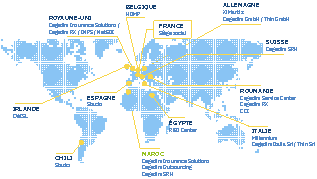
\includegraphics[width=\textwidth]{images/sec1/cegedim-presence-mondiale.pdf}
    \caption{Présence mondiale du groupe cegedim}
    \label{fig:international_presence}
\end{figure}

\subsubsection{Domaines d'activité}
Alliant maîtrise technologique des données, du numérique et des réseaux, les activités du groupe Cegedim se déclinent autour de \textbf{quatre divisions} opérationnelles. Ce découpage vise à améliorer la compréhension des activités en mettant en évidence les différents métiers exercés pour lesquels le lecteur disposera aisément de comparables connus sur le marché.\newline
\fboxsep=10pt\relax\fboxrule=2pt\relax%

\specialbox{white}{actBlue}{40pt}{0.50\textwidth}{
\begin{center}
  
\includegraphics[width=0.25\textwidth]{images/sec1/logiciels-et-services.pdf}  
\end{center}
{\footnotesize
regroupe l’ensemble des offres logiciels du Groupe sous toutes leurs formes (licence, SaaS, services internet) ainsi que l’hébergement (agrément HDS) et l‘infogérance. Cegedim cible l’assurance santé et prévoyance (France et Royaume-Uni), les professions paramédicales : kinésithérapeutes, infirmiers, orthophonistes, orthoptistes, podologues, sages-femmes… (France), les directions des ressources humaines (France), les pharmacies indépendantes, groupements ou chaînes de pharmacies (France, Roumanie et Royaume-Uni), les médecins et centres de santé (France, Royaume-Uni, Belgique, Espagne, Italie)\\\\}
\begin{tblr}
{ 
 rows = {bg=azure9},
 colsep=4pt,
 abovesep=4pt,
 row{2}={abovesep={8pt}},
 colspec={Q[r]Q[l]},
 rowspec={Q[m]Q[m]},
 vline{2} = {2pt,actBlue},
 }
{\Large \textcolor{actBlue}{\textbf{ 277,2 M€}}} &  CA 2020 \\
{\Large \textcolor{actBlue}{\textbf{ 55,8\%}}} &  CA groupe
\end{tblr}
}
\specialbox{white}{actPurple}{40pt}{0.50\textwidth}{
\begin{center}

\includegraphics[width=0.25\textwidth]{images/sec1/data-and-marketing.pdf}
\end{center}
{\footnotesize
regroupe les activités :
\begin{itemize}[itemsep=6pt]
    \item Données pour les autorités de santé, les professionnels de santé, les chercheurs, l’industrie de santé et ses partenaires en France, Italie, Allemagne, Espagne, Roumanie et Royaume-Uni ;
    \item Communication en pharmacie et parapharmacie d’enseigne en France sous format papier et numérique ;
    \item Marketing digital auprès des médecins ;
    \item Distribution de produits de santé.\\\\
\end{itemize}
}
\begin{tblr}
{ 
 rows = {bg=violet9},
 colsep=4pt,
 abovesep=4pt,
 row{2}={abovesep={8pt}},
 colspec={Q[r]Q[l]},
 rowspec={Q[m]Q[m]},
 vline{2} = {2pt,actPurple},
 }
{\Large \textcolor{actPurple}{\textbf{ 87,8 M€}}} &  CA 2020 \\
{\Large \textcolor{actPurple}{\textbf{ 17,7\%}}} &  CA groupe
\end{tblr}
}
\specialbox[t]{white}{actGreen}{40pt}{0.50\textwidth}{
\begin{center}

\includegraphics[width=0.25\textwidth]{images/sec1/flux.pdf}
\end{center}
{\footnotesize
regroupe les activités de gestion du tiers payant (France), de dématérialisation de processus et factures, d’archivage à valeur probante et d’EDI (France, Royaume-Uni, Allemagne). Pour cette activité Cegedim dispose de centres de services en France, Roumanie et Maroc.\\\\}
\begin{tblr}
{ 
 rows = {bg=teal9!50!white},
 colsep=4pt,
 abovesep=4pt,
 row{2}={abovesep={8pt}},
 colspec={Q[r]Q[l]},
 rowspec={Q[m]Q[m]},
 vline{2} = {2pt,actGreen},
 }
{\Large \textcolor{actGreen}{\textbf{ 79,4 M€}}} &  CA 2020 \\
{\Large \textcolor{actGreen}{\textbf{ 16,0\%}}} &  CA groupe
\end{tblr}}
\specialbox{white}{actPink}{40pt}{0.50\textwidth}{
\begin{center}

\includegraphics[width=0.25\textwidth]{images/sec1/BPO.pdf}
\end{center}
{\footnotesize
  regroupe les activités de Business Process Outsourcing en France pour le compte des assureurs complémentaires santé (entre autre gestion des remboursements) et institutions de prévoyance, et départements RH. Pour cette activité Cegedim dispose de centres de services en France et en Roumanie.\\\\}
  \begin{tblr}
{ 
 rows = {bg=purple9},
 colsep=4pt,
 abovesep=4pt,
 row{2}={abovesep={8pt}},
 colspec={Q[r]Q[l]},
 rowspec={Q[m]Q[m]},
 vline{2} = {2pt,actPink},
 }
{\Large \textcolor{actPink}{\textbf{ 48,9 M€}}} &  CA 2020 \\
{\Large \textcolor{actPink}{\textbf{ 9,8\%}}} &  CA groupe
\end{tblr}
 }
\par\bigskip
\begin{beware}[title=Note : ]
Cette ventilation par division présentée ci-dessus est la typologie privilégiée dans les communiqués de presse et les présentations financières de Cegedim. Il existe encore une cinquième division (non présentée ci-dessus), il s'agit de la division \textbf{Corporate et autres} et regroupe à la fois des activités inhérentes au statut de tête de Groupe coté, et des activités de support aux divisions du Groupe.
Cette division a réalisé en 2020 un chiffre d'affaires de 3,7 millions d'euros
(0,7\% du chiffre d'affaires consolidé du groupe). 

\end{beware}
\subsection{Cegedim SRH}
\subsubsection{Présentation}
Cegedim SRH, filiale du Groupe Cegedim, est l'un des leaders français des solutions et services de gestion de la paie et des ressources humaines. Acteur majeur du Cloud RH et des services externalisés, 
Cegedim SRH dispose d'une expertise de plus de 25 ans dans ce domaine accumulée et reflétée dans sa plateforme \textbf{TEAMS\textsuperscript{RH}} qui offre une large couverture fonctionnelle de solutions dédiées aux Ressources Humaines.\\
\begin{figure}[H]
    \centering
    
\includegraphics[width=0.25\textwidth]{images/sec1/cegedim-srh.pdf}
    \caption{Logo Cegedim SRH}
\end{figure}
La société compte parmi ses clients des entreprises nationales et internationales, de tous secteurs d’activité, issues des grands comptes et du mid-market.
\begin{figure}[H]
    \centering
    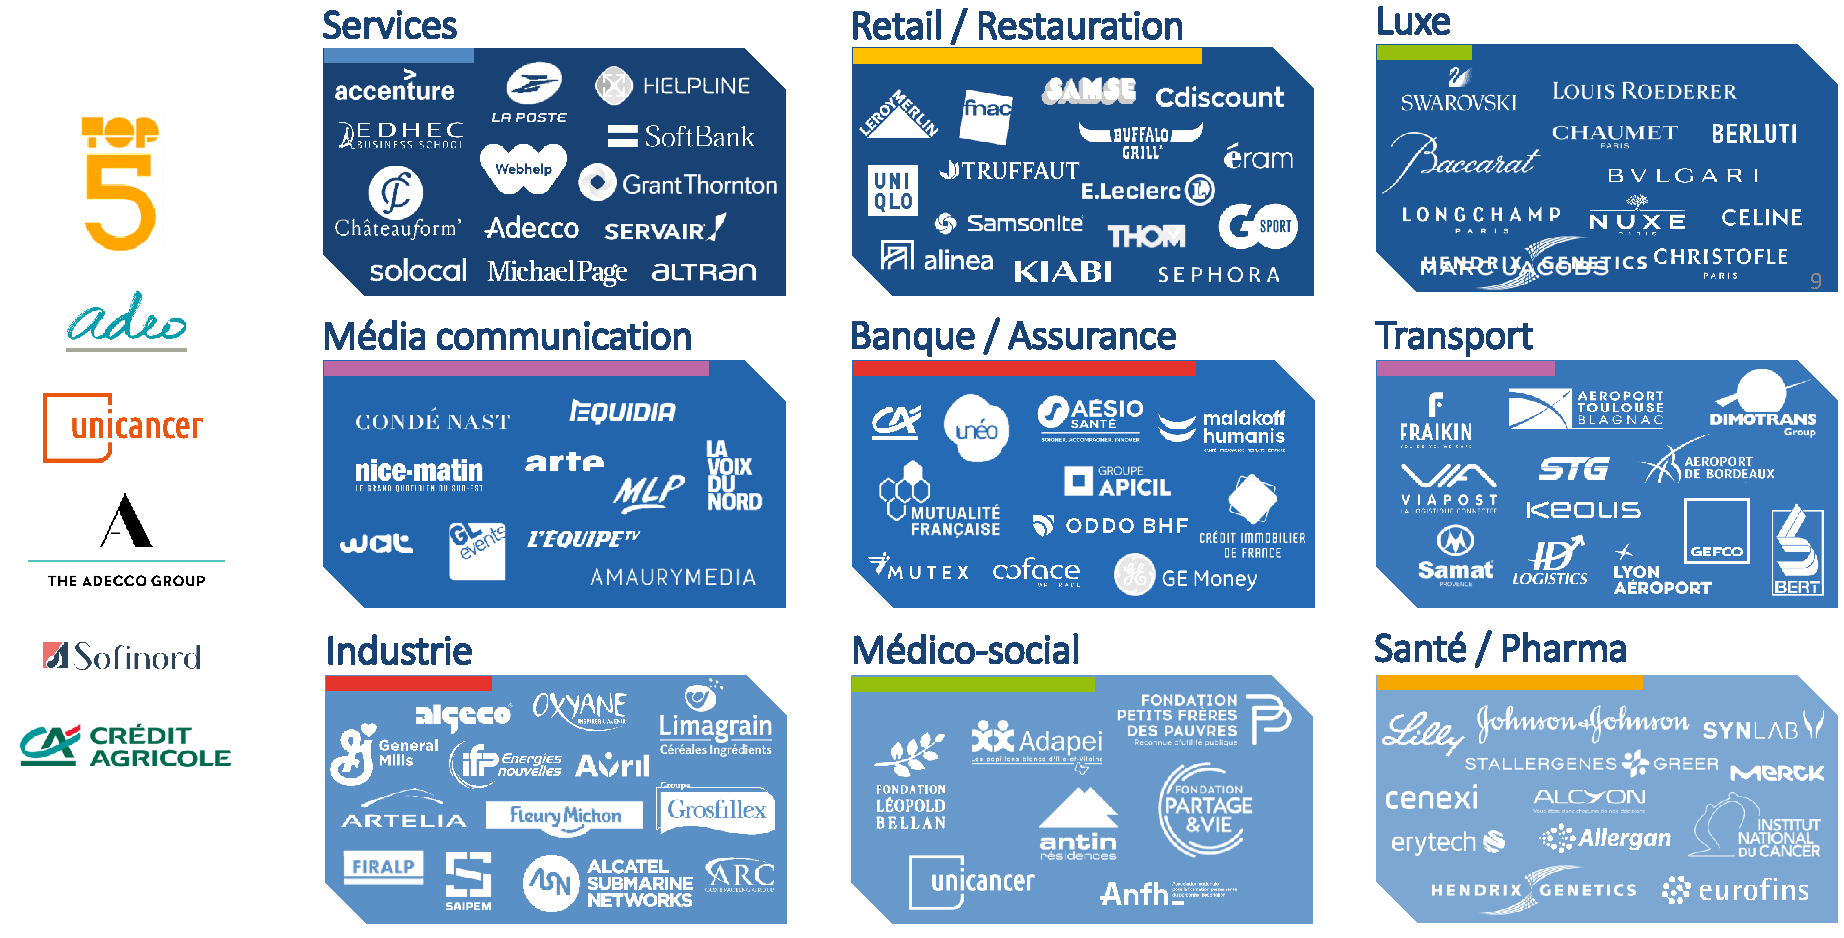
\includegraphics[width=\textwidth]{images/sec1/clients-cegedim-srh.pdf}
    \caption{Clients Cegedim SRH}
\end{figure}
\subsubsection{Domaines fonctionnels}
Capitalisant sur l'apport des nouvelles technologies, Cegedim SRH s'appuie sur un investissement continu et une stratégie de différenciation pour réinventer les outils de gestion RH à travers son offre TEAMS\textsuperscript{RH}, un SIRH complet et modulaire de solutions et services en mode externalisé pour répondre aux besoins d'agilité, de fiabilité et de performance de ses clients.
La plateforme TEAMS\textsuperscript{RH} est constituée d'un ensemble de modules tels que :

\begin{itemize}
    \item paie et gestion administrative,
    \item portail RH collaboratif,
    \item gestion des temps et des activités,
    \item pilotage social,
    \item gestion des RH (Entretiens et Formations),
    \item processus RH dématérialisés intégrés dans la solution (signature électronique et coffres-forts numériques).
\end{itemize}
\newpage
Pour aider ses clients à améliorer la performance de leurs activités, Cegedim SRH propose des services de gestion de la paie et des RH selon quatre niveaux de prestations, en fonction du degré de responsabilité de chaque acteur :\\ 

\vspace*{\fill}
\specialbox{white}{azure5}{40pt}{0.9\textwidth}{
{
\square{azure9}
\color{azure5}
\textbf{SaaS +}\\\\
}
abonnement aux services hébergés de TEAMS\textsuperscript{RH} incluant la maintenance corrective et les mises à jour légales et conventionnelles de l’application.\\}
\par\bigskip
\specialbox{white}{azure5}{40pt}{0.9\textwidth}{
{
\square{azure9} \square{azure8}
\color{azure5}
\textbf{Processing}\\\\
}
externalisation partielle avec pilotage de la relation client, le suivi du traitement de la paie, des opérations d’exploitation, de production et d’éditique.\\}
\par\bigskip
\specialbox{white}{azure5}{40pt}{0.9\textwidth}{
{
\square{azure9} \square{azure8} \square{azure7} 
\color{azure5}
\textbf{BPO on demand}\\\\
}
service d'externalisation de la paie évolutif et sur-mesure.\\}
\par\bigskip
\specialbox[t]{white}{azure5}{40pt}{0.9\textwidth}{
{
\square{azure9} \square{azure8} \square{azure7} \square{azure6}
\color{azure5}
\textbf{BPO}\\\\
}
externalisation complète avec prise en charge de l’ensemble des opérations de traitement de la paie (accréditation ISAE 3402).\\}
\vspace*{\fill}
\clearpage
\subsubsection{Agences et centres de services}
Cegedim SRH dispose de sites de proximité à Paris, Lyon, Lille, Nantes et Toulouse, associés à des centres de développement nearshore à Montargis, Vichy et Genève, et offshore à Bucarest et Rabat (voir figure ~\ref{fig:sites_cegedim}).
\begin{figure}[H]
    \centering
    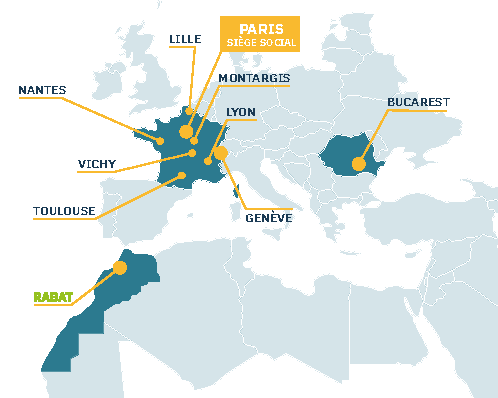
\includegraphics[width=0.78\textwidth]{images/sec1/cegedim-srh-map2.pdf}
    \caption{Les différents sites SRH}
    \label{fig:sites_cegedim}
\end{figure}
\subsubsection{Organigramme SRH}
Cegedim SRH dispose d’un organigramme qui montre sa structure générale ainsi que l’organisation de ses directions.
\tikzset{
        basic/.style={draw=none, text width=12em, rectangle,font=\bfseries, inner sep=0.25cm, outer sep=0cm,rounded corners=3pt},
        titre/.style={basic, align=center, minimum height=4em, text=azure3, fill=white,draw},
        objectif/.style={basic, align=center, anchor=north, text width=7.5em, minimum height=4.375em, text=azure3, fill=azure9, font=\footnotesize},
        specification/.style={basic, align=left, anchor=center, fill=alice, text width=6.25em, minimum height=3em,text=hoki,font=\footnotesize\bfseries}
    }

\begin{figure}[H]
\centering
 \resizebox{\linewidth}{!}{
   \begin{tikzpicture}[level distance=6em,line width=1pt,gray9,level 1/.style={sibling distance=10em},
    edge from parent path={(\tikzparentnode.south) |- (0em,2em) -| (\tikzchildnode.north)},
    edge from parent/.style={draw},on grid,node distance=2.25cm
    ]% <----- New options on grid and node distance
        \node [titre] {Cegedim SRH}
            child {node [objectif] (o1) {\textbf{Offre et R\&D}}}
            child {node [objectif] (o2) {\textbf{Développement commercial}}}
            child {node [objectif] (o3) {\textbf{Opérations}}}
            child {node [objectif] (o4) {\textbf{Externalisation de services et des TPE/PME}}}
            child {node [objectif] (o5) {\textbf{Satisfaction client et contrôle interne}}}
        ;
        \begin{scope}[every node/.style=specification]
            \node [below=of o1] (o11) {Offre};
            \node [below=of o11] (o12) {Développement technique};
            \node [below=of o12] (o13) {Fonctionnel Paie et\\Juridique};
            \node [below=of o13] (o14) {Fonctionnel RH};
            \node [below=of o14] (o15) {Technique et dev spécifiques};
            \node [below=of o15] (o16) {Qualité \&\\ Documentation};
            \node [below=of o2] (o21) {Marketing\\opérationnel};
            \node [below=of o21] (o22) {Avant-vente};
            \node [below=of o22] (o23) {Chasse};
            \node [below=of o23] (o24) {Parc};
            \node [below=of o3] (o31) {Boulogne};
            \node [below=of o31] (o32) {Lyon};
            \node [below=of o32] (o33) {Nantes};
            \node [below=of o33] (o34) {Lille};
            \node [below=of o34] (o35) {Toulouse};
            \node [below=of o35] (o36) {Centre de \\services};
            \node [below=of o4] (o41) {Rue de la Paye};
            \node [below=of o41] (o42) {BPO Bucarest};
            \node [below=of o42] (o43) {BPO/TPO\\Montargis et Boulogne};
            \node [below=of o43] (o44) {BPO Vichy};
            \node [below=of o44] (o45) {Projets TPO};
            \node [below=of o5] (o51) {Formation};
            \node [below=of o51] (o52) {AMOA et\\Assistance};
            \node [below=of o52] (o53) {RH};
            \node [below=of o53] (o54) {OPEX};
            \node [below=of o54] (o55) {Finances};
            \node [below=of o55] (o56) {Fabex};
        \end{scope}
        \foreach \value in {1,...,6}
            \draw (o1.west) -- ++(-0.5em,0em) |- (o1\value.west);
        \foreach \value in {1,...,4}
            \draw (o2.west) -- ++(-0.5em,0em) |- (o2\value.west);
        \foreach \value in {1,...,6}
            \draw (o3.west) -- ++(-0.5em,0em) |- (o3\value.west);
        \foreach \value in {1,...,5}
            \draw (o4.west) -- ++(-0.5em,0em) |- (o4\value.west);
        \foreach \value in {1,...,6}
            \draw (o5.west) -- ++(-0.5em,0em) |- (o5\value.west);
    \end{tikzpicture}
}
    \caption{Organigramme des Directions Cegedim SRH au 1er janvier 2019}
    \label{fig:organigramme_cegedim_srh}
\end{figure}
%%%%%%%%%%%%%%%%%%%%%%%%%%%%%%%%%%%%%%%%%%%%%%%%%%%%
%% Présentation du projet
%%%%%%%%%%%%%%%%%%%%%%%%%%%%%%%%%%%%%%%%%%%%%%%%%%%
%%%%%%%%%%%%%%%%%%
\section{Présentation du projet}
\addcontentsline{toc}{subsection}{Introduction}
\subsection*{Introduction}
Dans ce présent chapitre, nous nous articulerons sur l’étude et l’analyse du projet.
Pour ce faire, nous débuterons par une étude préalable dans laquelle nous exposerons les fonctionnalités de la GED et ses avantages compte tenu de son implication dans le sujet, puis nous entamerons une étude du système existant, pour ensuite identifier les problèmes, les points à améliorer et les solutions envisagées.
\subsection{Étude préliminaire}
Avant d'entamer la discussion sur le sujet du stage, nous allons introduire quelques concepts et terminologie de la GED qui nous aideront à mieux comprendre le sujet par la suite.
\subsubsection{Qu'est-ce que la GED ?}
\begin{beware}[title=Définition : ]
    La GED ou Gestion Électronique de Documents est ensemble de logiciels concourant à réaliser les diverses étapes de la chaîne de traitement d’un document : acquisition, restitution, diffusion \cite{ged}.
    \end{beware}
    La GED est donc un système informatique qui vise à
    gérer et organiser les documents numériques (souvent issus de l'entreprise). En outre, la GED permet la numérisation des documents papier, ainsi que la dématérialisation des processus métier associés.\\La gestion électronique des documents utilise des outils et des fonctionnalités pour gérer toutes les étapes du cycle de vie d'un document numérique :
\begin{itemize}
    \item Création ou acquisition du document (ex : numérisation) ;
    \item Stockage, indexation et organisation du document électronique ;
    \item Gestion de la sécurité des données du document électronique ;
    \item Recherche, consultation du document électronique et échange des informations ;
    \item Archivage électronique du document durant son délai de conservation.
\end{itemize}
\subsubsection{Bénéfices d'une GED}
D’un point de vue stratégique, la mise en place d’une solution de GED rend possible une rationalisation des flux d’informations et donc un gain de temps. Elle permet notamment de :    
\begin{itemize}
    \item Éviter la duplication des processus et ainsi réduire les coûts de traitement.
    \item Éviter la perte de documents.
    \item Trouver facilement et rapidement la bonne version d’un document.
    \item Uniformiser les pratiques documentaires.
    \item Partager des données avec un certain nombre de personnes autorisées.\\
\end{itemize}

D’un point de vue plus opérationnel et technique, la GED garantit : 
\begin{itemize}
    \item La pérennité des documents et de leur support.
    \item L'interopérabilité : les documents peuvent être accessibles sur différentes plates-formes et pour des usages divers.
    \item La sécurité : l’accès aux données est sécurisé, la solution s’adapte aux différents profils utilisateurs.
    \item La traçabilité : retrouver les actions effectuées (dépôts, restitutions, demandes de copies, etc.)
\end{itemize}
\subsection{Étude de l'existant}
\subsubsection{Présentation du projet Arkevia}
\textbf{ARKEVIA} est  un service  innovant  et  pratique de coffre-fort  numérique  développé  par  Cegedim  SRH permettant aux salariés des entreprises adhérentes de recevoir et de conserver dans un espace sécurisé les bulletins de salaire et les communications institutionnelles en version électronique dans des conditions optimales de confidentialité et de sécurité. Arkevia permet également aux salariés de classer et de conserver leurs documents personnels importants tels que les pièces d'identité, les diplômes, les factures, etc.\\

Le coffre-fort Arkevia constitue un espace de stockage sécurisé pour les documents qui y sont déposés (EDI, EDI signé, PDF signé).\\
Il permet de garantir :
\begin{itemize}
    \item \textbf{Intégrité} : L'intégrité des documents, au moyen d’une fonction de signature électronique.
    \item \textbf{Confidentialité} : La confidentialité des documents, au moyen d’une fonction de chiffrement de données.
    \item \textbf{Traçabilité} : La traçabilité des actions effectuées (dépôts, restitutions, demandes de copies, etc.)
    \item \textbf{Vocation probante} : Les solutions de traçabilité constituent de vraies preuves juridiques basées sur leur intégrité, leur exhaustivité et leur opposabilité en cas de litige.\\
\end{itemize}
\newpage
\noindent
\textbf{Bénéfices pour le salarié :}
\begin{itemize}
    \item Accès illimité (24 h/7 j) depuis n’importe quel endroit grâce à une connexion Internet.
    \item Tous les bulletins de salaire déposés dans le coffre-fort ont la même valeur juridique que leur équivalent papier, même en cas de départ de l’entreprise.
    \item Espace personnel sécurisé de 1 Go dédié pour archiver les bulletins de paie et documents RH en version électronique pour une durée de conservation peut aller jusqu'à 50 ans des bulletins de salaire.
    \item Protection des documents importants contre le vol et la perte.
    \item Accès au coffre-fort sécurisé et garanti.\\
\end{itemize}

\noindent
\textbf{Bénéfices pour l’entreprise :}
\begin{itemize}
    \item Optimisation des processus RH d’éditique et de distribution documentaire.
    \item Réduction des coûts de distribution.
    \item Image moderne et innovante de la DRH.
    \item Enrichissement de l’expérience du salarié.
\end{itemize}
\subsubsection{Architecture globale d'Arkevia}
Terminologie nécessaire à la compréhension du sujet :
\begin{beware}[title=Terminologie : ] 
   \begin{itemize}
       \item \textbf{SignArchive} : application de la BU Cegedim e-business, hostée au  datacenter de Boulogne et exploitée par l’équipe interne, ayant pour but le stockage et la signature de documents numériques dans des services à valeur légalement probante.
       \item \textbf{Arkevia} : application Web, décrite dans ce document, présentant une  interface web publique consultable par un navigateur, dont le but est l'exploration et la manipulation de documents dans les coffres SignArchive.
       \item \textbf{Arkevia-SRH} : module d'extension pour Arkevia permettant la mise à disposition dans Arkevia de données (traductions, formulaires d’abonnement, conditions  d'utilisation) issues du système d’information de SRH. Ce module permet la prise en charge des abonnements des utilisateurs d’Arkevia au système de dématérialisation des bulletins de paie émis par SRH.
       \item \textbf{SignArchive-Batcher} : module de traitement générique pour les   applications souhaitant émettre des documents dans SignArchive, à des fins d’exploration par un utilisateur Arkevia.  Le système d’information de SRH utilise SignArchive-Batcher pour placer les bulletins dans les coffres.
   \end{itemize}
\end{beware}
\subsubsubsection{Généralités}
Le développement du produit SignArchive offre à la BU Cegedim e-business, ses clients et partenaires, l’occasion de disposer d’un produit capable à la fois :
\begin{itemize}
    \item de stocker des fichiers (de façon légalement probante si besoin) ;
    \item de les organiser par des métadonnées ;
    \item de fédérer des droits d’accès dynamiques autour de ces fichiers via une API standard (purement HTTP).
\end{itemize}
Au-delà de l’aspect juridique de ce logiciel d’archivage (exploité par les solutions de dématérialisation du groupe), le groupe dispose également d’un moteur de stockage, gestion, recherche et contrôle d'accès qui peut être mis à disposition de toute problématique orientée partage ou publication de document.\\

C’est à une de ces fonctions que s’attache  le projet  Arkevia,  dont  le périmètre fonctionnel est triple :
\begin{enumerate}
    \item Fournir un site web portant une offre de coffre-fort numérique à destination du (grand) public et exposé via le produit SignArchive. Ce site web s’appelle Arkevia.
    \item Offrir à des tiers la capacité de devenir « producteur de documents » pour le portail Arkevia, c’est-à-dire, définir les modalités techniques selon lesquelles un système d’information (interne ou externe) peut s’accrocher au portail Arkevia et à SignArchive,  de façon à ce que les clients d’Arkevia puissent visualiser des documents produits par des tiers.
    \item Implémenter un  tel « tiers producteur » pour les besoins de SRH, permettant la dématérialisation des bulletins de paie émis par l’entreprise.\\
\end{enumerate}

Le deuxième point définit clairement l'objectif d'extensibilité du système, ce qui détermine la plupart des choix de mise en œuvre effectués pour parvenir à la solution globale.

\subsubsubsection{Présentation métier}
La réalisation de la finalité du produit, à   cause de son besoin de généricité, est confiée à trois livrables distincts.
\begin{beware}[title=Note : ]
    La présence de ces trois produits est nécessaire au fonctionnement global de la solution Arkevia+SRH, mais Arkevia peut/aurait pu/pourrait tout à fait exister sans le module SRH, et réciproquement, le module SRH n’a pas besoin d’Arkevia pour pousser les fichiers dans les coffres SignArchive. D’autre part, le module SRH a été développé par Cegedim e-business à la demande de SRH, mais le produit est conçu de sorte qu’Arkevia puisse être implémenté par un producteur qui souhaite prendre en charge lui-même cette implémentation.
\end{beware}
\noindent
Ainsi, les fonctionnalités sont réparties comme suit :\\\\
\textbf{Arkevia}\\
Le site web Arkevia  propose à des navigateurs web en provenance d’internet, la consultation de coffres-forts  SignArchive dans  une interface  de navigation  proche d’un explorateur. Son rôle premier est  donc celui  de « proxy » SignArchive (se connecter pour le compte de l’utilisateur sur SignArchive), et de couche de présentation. D’autre part, Arkevia permet à ses utilisateurs de « s’abonner » à des « producteurs » de documents. La gestion de ces abonnements (présentation  du formulaire d’abonnement spécifique à un producteur, messages de notification du  producteur, ...) nécessite qu’Arkevia puisse communiquer avec le producteur pour échanger images, documents, données, etc. Cette communication doit respecter des principes techniques établis dans le cahier des charges d'implémentation d’Arkevia.\\\\
\textbf{Arkevia-SRH}\\
Ce livrable constitue le module d’abonnement du producteur SRH. Son rôle est :
\begin{enumerate}
    \item De gérer la liste des personnes autorisées à s’abonner au producteur SRH ; et d'en rendre compte à SRH.
    \item De fournir à Arkevia les éléments nécessaires à la  présentation  et la  prise en compte des données d’abonnement (champs de formulaire à  présenter pour s'inscrire, libellés traduits des messages affichés par \textbf{Arkevia} pour le compte de SRH, etc.).
\end{enumerate}

Il est donc constitué à la fois d’une chaîne de traitement chargée de la prise en compte des données d’inscription publiées par SRH, et de web services de publication de données.\\\\
\textbf{SignArchive-Batcher}\\
Ce livrable est une chaîne de traitement publiant, pour le compte de SRH, les bulletins de salaire à dématérialiser dans \textbf{SignArchive}, selon le format admissible pour \textbf{Arkevia}.\\\\
\subsubsubsection{Vue d’ensemble}
Au global, on a une répartition des tâches sous la forme schématique suivante (voir figure  ~\ref{fig:architecture_arkevia}) :
\begin{figure}[H]
    \begin{center}
        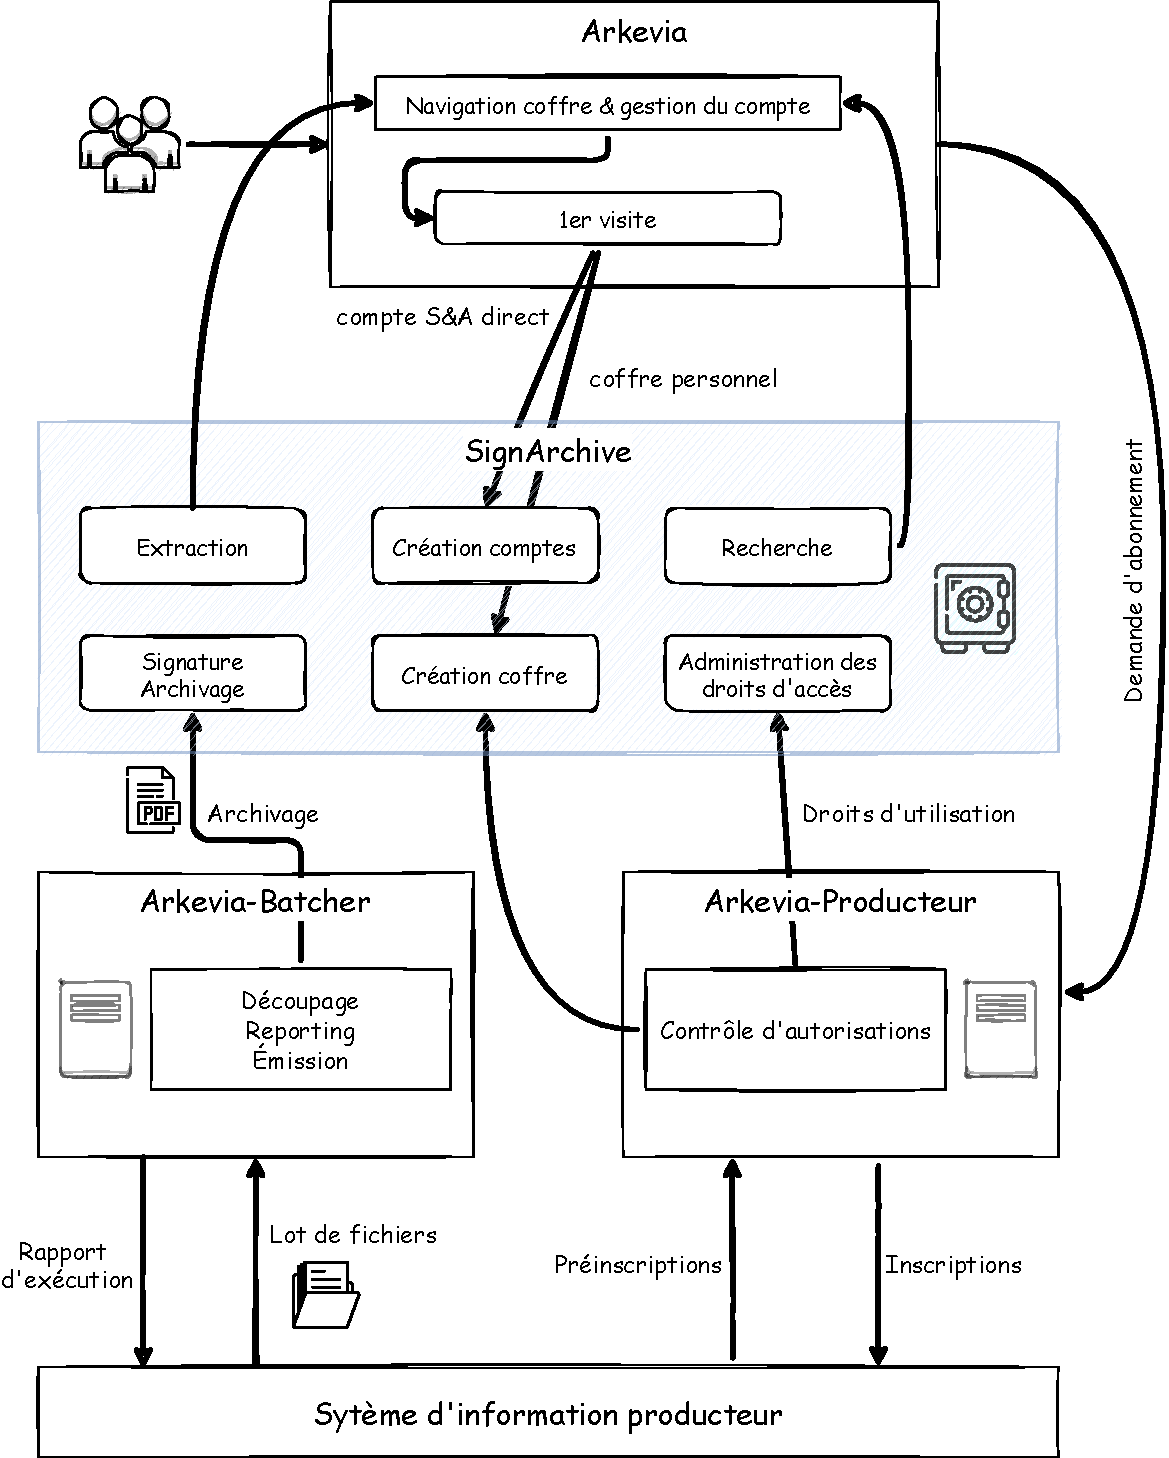
\includegraphics[width=\linewidth]{images/sec2/architecture-globale.pdf}
        \caption{Répartition des tâches dans l'écosystème Arkevia}
        \label{fig:architecture_arkevia}
    \end{center}
\end{figure}
\newpage

\begin{enumerate}
    \item  \textbf{Arkevia} se connecte à \textbf{SignArchive} pour en afficher le contenu, indépendamment du fait que SRH publie ou non des documents pour cet utilisateur. Cependant, si l’utilisateur souhaite s’abonner au service de production SRH, alors, Arkevia pousse la demande via un web service au module approprié, \textbf{Arkevia-SRH}.

    \item \textbf{Arkevia-Producteur (Arkevia-SRH)} peut prendre en compte ou non la demande, selon les autorisations qui lui ont été publiées par SRH directement, via le fichier des préinscriptions. Chaque inscription ou résiliation est remontée à SRH via le même canal que le fichier des préinscriptions.

    \item En conséquence de quoi, lors de la fabrication des bulletins de paie, le module de gestion interne à SRH peut constituer une archive des bulletins à archiver conforme aux utilisateurs Arkevia inscrits. Ce fichier est poussé au module \textbf{SignArchive-Batcher} qui pousse les fichiers dans \textbf{SignArchive}.
\end{enumerate}
\subsection{Problèmes et axes d'amélioration}
\subsubsection{Défis technologiques}
Le backend de l'application Arkevia est développé principalement avec la technologie Spring 3.x. Ce framework a été publié pour la première fois en 2004 et a subi de nombreuses révisions depuis lors : 
\begin{itemize}
    \item Spring 2.0 a fourni des espaces de noms XML et le support d'AspectJ ; 
    \item Spring 2.5 a adopté la configuration basée sur les annotations ; 
    \item Spring 3.0 a introduit une solide base Java 5+ à travers le socle du framework et des fonctionnalités telles que le modèle @Configuration basé sur Java.\\
\end{itemize}

Aujourd'hui, le projet Spring et le développement Java ont tous deux évolué de manière significative, incluant à la fois des correctifs de sécurité et de nouvelles fonctionnalités et améliorations, faisant de la migration une tâche assez importante.

À cet égard, il a été convenu de réaliser une étude comparative sur l'impact d'une telle migration du framework Spring ; le résultat de cette étude fera l'objet d'un travail de développement sur la migration du socle technique d'Arkevia.

\subsubsection{Refactorisation et nettoyage du code}
Comme mentionné dans l'introduction, le portail Arkevia a subi plusieurs changements et évolutions au cours des dernières années, rendant le code trop compliqué, redondant et imprégné de mauvaises odeurs (code smells), d'où la nécessité de recourir à un processus de refactoring et d'amélioration du code tout en préservant les fonctionnalités existantes. Le but est de transformer un code inefficace et compliqué en un code plus efficace, de préférence plus simple et plus clair.
\subsubsection{Mécanisme de Notification}
Le mécanisme d'envoi de notifications est responsable de notifier un utilisateur par mail, lorsqu'il y a un nouveau dépôt de document (Bulletin de paie, note de frais, etc.) sur son coffre-fort par la société à laquelle il appartient.\\

Le module de gestion de l'envoi des notifications est intégré à l'application mère Arkevia. Le processus d'envoi est planifié pour être déclenché toutes les deux heures, et à chaque exécution, l'application Arkevia sollicite le service chargé d'interroger l'API SignArchive pour récupérer la liste des documents déposés et celle des utilisateurs associés afin de préluder à l'envoi des notifications.
Le mécanisme actuel n'est pas capable à traiter la volumétrie de documents en production. En effet, ce dernier souffre de plusieurs failles et notamment quand le nombre de documents déposés dans SignArchive est élevé, le système se met à défaillir et à dysfonctionner, ce qui entraîne que certains utilisateurs ne reçoivent plus les notifications sur la présence des documents déposés dans leur coffre-fort ou les reçoivent plusieurs fois pour un même document, etc. 

\subsection{Objectif de la refonte}
L'objectif est de revoir, corriger et améliorer / traiter les problèmes et les axes d'amélioration identifiés suite à l'audit d'architecture effectué.

Avec un refactoring continu qui adopte une approche progressive, le produit reste utilisable, contrairement à un logiciel qui doit être entièrement réarchitecturé, voire redéveloppé. Comme je l’ai dit, je pense que c’est la meilleure option pour pérenniser un produit digital mais ce n’est pas une solution miracle. Elle demande du temps et des compétences, quitte à reporter le développement de certaines nouvelles fonctionnalités.

Si je peux donner un conseil sur l’organisation, ce serait de garder un temps au refactoring de code dans chaque itération et quand c’est nécessaire lui réserver une itération.
\addcontentsline{toc}{subsection}{Conclusion}
\subsection*{Conclusion}
%%%%%%%%%%%%%%%%%%%%%%%%%%%%%%%%%%%%%%%%%%%%%%%%%%%


%%%%%%%%%%%%%%%%%%%%%%%%%%%%%%%%%%%%%%%%%%%%%%%%%%%
%% Éléments flottants
%%%%%%%%%%%%%%%%%%%%%%%%%%%%%%%%%%%%%%%%%%%%%%%%%%%
%%%%%%%%%%%%%%%%%%
\section{Méthodologie de gestion de projets}
\addcontentsline{toc}{subsection}{Introduction}
\subsection*{Introduction}
Dans ce chapitre, nous aborderons les aspects de la gestion de projet, de la composition des équipes, des outils et des méthodes de développement de logiciels adoptés par Cegedim SRH.
\subsection{Étude préliminaire}
\subsubsection{Origine du génie logiciel}
\begin{beware}[title=Définition : ]
Le génie logiciel est la science de l'ingénieur qui s'intéresse aux procédés scientifiques de construction et d'entretien des logiciels, et bien évidemment à la « matière » même de cette construction : d'abord les programmes eux-mêmes, les fichiers et bases de données, les scripts de paramétrage nécessaires à l'exécution du programme, puis tout ce qui gravite autour (spécification de besoins et exigences des futurs utilisateurs, conception, tests, documentation pour les mainteneurs, le support technique et les usagers)\cite{origine_gl1}.
\end{beware}

À la fin des années 50, l’informatique est devenue de plus en plus populaire et s’est étendue à d’autres disciplines. Ceci en raison de l’impulsion des grands projets spatiaux et militaires, grands consommateurs de logiciels et imposant des exigences de qualité et de sûreté de fonctionnement et du fait que les informaticiens du génie logiciel étaient plus enclins et plus à même de développer des outils logiciels d’aide à la conduite des activités.\\

En octobre 1968, l'OTAN a organisé une première conférence, à Partenkirchen en Allemagne, sur l’industrialisation de l’élaboration du logiciel. C’est à cette occasion qu'est forgée l’expression « Software Engineering » pour donner une tournure délibérément industrielle au propos\cite{origine_gl3}.\\

À la fin des années 60, les grands systèmes commerciaux ont démontré qu'il était difficile d'adapter à grande échelle les principes qui avaient été adéquats jusque là. Les grands projets dépassaient les budgets et les délais, ce fût alors « the software crisis » la crise du logiciel\cite{origine_gl2}.\\

La conférence de l'OTAN a été immédiatement suivie par de nombreuses autres conférences portant sur des thèmes liés au génie logiciel, tels que la fiabilité des logiciels, le test du logiciel, la spécification du logiciel, la maintenance du logiciel, etc.

En 1975 s'est tenue la première conférence véritablement dédiée à l’ensemble du génie logiciel, accompagnée d'une exposition de premiers outils, notamment pour l’aide au test. Depuis, l’IEEE tient une rencontre annuelle internationale. Cette première conférence a correspondu à la création, au sein de l’IEEE, d’un comité technique dédié au génie logiciel, animateur d’une série de conférences et ateliers récurrents et éditeur de deux revues dédiées au génie logiciel\cite{origine_gl3}.
\subsubsection{Comparaison des différentes méthodes de développement}
\subsubsubsection{Les approches traditionnelles}
Dans une approche traditionnelle, le cycle de vie d'un logiciel passe par quatre phases principales : \textbf{initiation}, \textbf{développement}, \textbf{déploiement} et \textbf{exploitation}.
\begin{itemize}
    \item \textbf{L'initiation} vise à déterminer la mission du système et à effectuer des travaux exploratoires permettant de vérifier la pertinence du projet.
    \item \textbf{Le développement} est la phase qui prend en charge la réalisation du logiciel. Elle précise les besoins, réalise le produit et valide son fonctionnement.
    \item \textbf{Le déploiement} rend le produit accessible à ses utilisateurs, par la mise en service du logiciel dans son environnement de production.
    \item \textbf{L’exploitation} est la période de vie utile du produit au cours de laquelle des améliorations peuvent être apportées au produit.
\end{itemize}

% Un ensemble d’éléments est nécessaire à un projet conduit par une approche traditionnelle. 
% La table ~\ref{tab:trad} résume les phases et les principales tâches qu’elles regroupent.

% \begin{longtblr}[caption={Description des étapes du cycle de vie logiciel dans une apporche traditionnelle},label={tab:trad}]{
%     hlines = {0.25pt,azure6},
%     vlines = {0.25pt,azure6},
%     row{odd} = {bg=azure9!10!white},
%     colsep=4pt,
%     rowsep=4pt,
% 	colspec={cX},
%     rowspec={Q[m] Q[m] Q[m] Q[m] Q[m] Q[m] Q[m] Q[m] Q[m] Q[m] Q[m] Q[m] Q[m] Q[m] Q[m] Q[m] Q[m] Q[m] Q[m] Q[m] Q[m]},
%     cell{1}{2} = {c},
%     cell{2}{1} = {c=2}{c,azure7},
%     cell{5}{1} = {c=2}{c,azure7},
%     cell{12}{1} = {c=2}{c,azure7},
%     cell{18}{1} = {c=2}{c,azure7},
% }
% \textbf{Étapes}&\textbf{Description}\\
% \textbf{Initiation}\\
% Étude de faisabilité
%  & L'ÉTUDE DE FAISABILITÉ produit un document qui analyse les besoins et définit le mandat et les limites du système.\\
%  Planification du projet
% & 
% LE PLAN DE PROJET présente à travers le temps les différentes phases du projet, il
% précise ses ressources, son délai et son coût.\\
% \textbf{Développement}\\
% {Analyse et spécifications
% \\des besoins}
% & 
% LES SPÉCIFICATIONS REQUISES analysent et précisent les qualités internes requises pour juger de la conformité du produit. 
% \\
% {Spécification du design
% \\(Architecture)}
% &  LES SPÉCIFICATIONS DU DESIGN, correspondent à la décomposition en modules et les relations qu’ils ont entre eux.\\
% Analyse fonctionnelle
% &  L’ANALYSE FONCTIONNELLE détaille les unités de programmation à leur plus bas niveau, avant d’être codé. L’ensemble des éléments doit précisément y être spécifié. On y retrouve les maquettes d’écran, les données exploitées et le détail des algorithmes.\\
% {Programmation et tests
% \\unitaires}&La programmation réalise Le Code Source, qui est le livrable de cette étape. UN PLAN DE TESTS UNITAIRES doit aussi être produit pour valider le code.\\
% {Intégrations et tests
% \\systèmes}& L’intégration consiste à valider l’interaction des unités de programmation ensemble.
% UN PLAN DES TESTS SYSTÈMES prévoit la vérification des échanges entre les unités et les modules du système. Les interfaces modulaires sont testées à ce niveau.\\
% Documentation & La documentation explique comment exploiter l’application. La DOCUMENTATION TECHNIQUE est destinée à l’administration du système et la DOCUMENTATION DIDACTIQUE est destinée aux utilisateurs, elle est utilisée lors des sessions de formation. \\
% \textbf{Déploiement}\\
% Plan de déploiement & L’implantation est l’étape de livraison du produit au client. Le logiciel doit être installé sur les machines de production réelle. LE PLAN D’IMPLANTATION guide les étapes à suivre pour procéder à cette mise en service.\\
% Formation & Les utilisateurs doivent être formés sur le nouveau système, afin qu’ils connaissent les fonctionnalités disponibles dans leur nouveau système. LE PLAN DE FORMATION détaille la stratégie et les moyens utilisés.\\
% Conversion de données & Cette étape sert à alimenter le nouveau système à partir de données existantes. Celles-ci doivent être converties dans un nouveau format. UN PLAN DE CONVERSION doit être produit afin de spécifier les interfaces d’importation et l’exportation des données existantes.\\
% Tests d'acceptation & Les tests d’acceptation sont réalisés par les pilotes ou les utilisateurs, afin de d’approuver le système. UNE LISTE DES DEMANDES DE CORRECTIONS est rédigée dans le but de corriger les éléments non conformes aux attentes du client.\\
% Vérification posthume & 
% Lors de la fermeture du projet de développement, une vérification posthume révise le déroulement des différentes étapes. LE RAPPORT DE FIN DE PROJET explique les difficultés rencontrées et les bonnes pratiques à retenir.\\
% \textbf{Exploitation}\\
% {Suivi Opérationnel 
% \\et support} & Le suivi opérationnel assure le fonctionnement du système. Des éléments de surveillance permettent de contrôler le fonctionnement. Le support consiste à répondre aux questions et à compléter la formation auprès de l’équipe en charge de l’exploitation ou des utilisateurs.\\
% Maintenance & La maintenance du système permet de corriger les erreurs de conception et de
% compléter ou d’ajouter des fonctionnalités\\

% {Décisions récurrentes :
% \\Continuer – Refaire -
% \\Terminer} & Le système doit être évalué de manière récurrente pour confirmer sa pertinence. À travers le temps, de nouvelles opportunités peuvent comporter suffisamment d’avantages pour abandonner un système désuet. 

% \end{longtblr}

\subsubsubsection{Les méthodes agiles}
Une méthode agile est une approche itérative et incrémentale, qui est menée dans un esprit collaboratif, avec juste ce qu’il faut de formalisme. Elle génère un produit de haute qualité tout en prenant en compte l’évolution des besoins des clients\cite{agile1}.\\

Le Manifeste Agile déclare quatre valeurs dans toute approche agile. Chaque méthode adopte ensuite sa propre terminologie et recommande un certain nombre de pratiques. Les quatre valeurs du Manifeste sont\cite{agile1, agile4} :
\begin{itemize}
    \item Les individus et leurs interactions avant les processus et les outils. 
    \item Des fonctionnalités opérationnelles avant la documentation.
    \item Collaboration avec le client plutôt que contractualisation des relations. 
    \item Acceptation du changement plutôt que conformité aux plans.
\end{itemize}

\subsubsubsection{Synthèse}
Bien que les approches traditionnelles présentent divers avantages, elles ont aussi certaines limites, en particulier dans les environnements évolutifs. En effet, les environnements évolutifs nécessitent des adaptations constantes. Avec une planification rigoureuse, il est difficile d’apporter des changements à cause de leurs impacts, et plus un changement est fait tard, plus il est coûteux. Cette situation tardive exige de modifier l'enchaînement des étapes antérieures et seuls les changements les plus importants seront opérés.\\

% Certains projets peuvent requérir moins d’effort de gestion. Les suivis et les rapports alourdissent la charge administrative. Les communications écrites sont coûteuses et longues à produire. Il faut tenir compte de l’ampleur et de la complexité du projet. Si le produit est livré dans un délai important, il est possible que la situation du client ait évolué et que l’on soit appelé à modifier le système.\\

Selon une nouvelle étude menée par Organize Agile\cite{organize_agile} auprès de professionnels de 19 pays, près de la moitié des organisations utilisent des méthodes agiles depuis trois ans ou plus. Ces entreprises utilisent principalement Agile comme méthodologie pour leurs programmes de réforme - connus sous le nom de transformations agiles. Il s'agit de grands changements organisationnels qui adoptent le travail agile au sein de petites équipes multidisciplinaires qui s'attachent à fournir des résultats de manière rapide, expérimentale et itérative, ce qui révèle l'impact positif de ces méthodes sur les flux de travail des projets informatiques à l'échelle mondiale. Au Maroc, selon un rapport d'étude mené en 2011 impliquant 48 organisations participantes représentant les secteurs privé et public a révélé que le taux de satisfaction de la maîtrise d'ouvrage est plus élevé pour les DSI adoptant une des méthodes agiles ce qui démontre leur pragmatisme et leur efficacité par rapport aux méthodes traditionnelles en cascade\cite{badr_2011}.\\

Les approches agiles et traditionnelles convergent et divergent sur différents aspects. L’expérience de l’équipe peut faire diminuer les risques et contribuer à minimiser les exigences de suivi. Les approbations et le manque d’autonomie des équipes peuvent ralentir le projet. Une organisation peu hiérarchisée, ayant une culture collégiale, intégrera difficilement une structure traditionnelle.\\
\subsection{Conduite de projet}
\subsubsection{Modèle de livraison}
Aujourd'hui, Cegedim adopte une approche de livraison agile que tout projet est censé suivre. Le schéma ci-dessous montre les différentes phases de ce modèle (voir figure  ~\ref{fig:delivery}) :
\begin{figure}[H]
    \begin{center}
        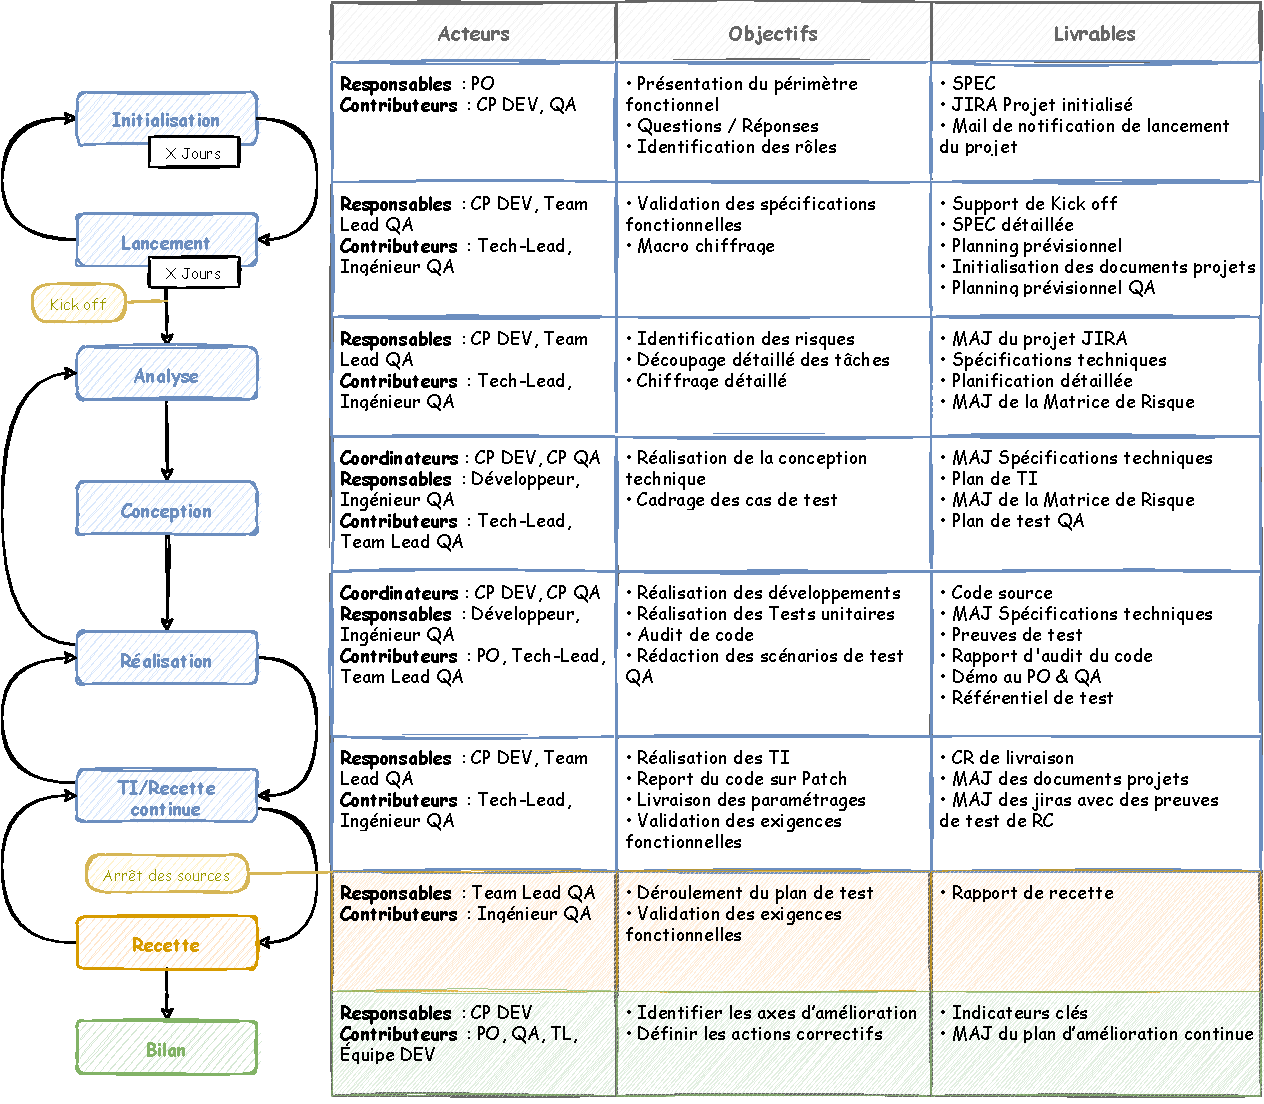
\includegraphics[width=\linewidth]{images/sec3/deliveryprocess.pdf}
        \caption{Modèle de livraison}
        \label{fig:delivery}
    \end{center}
\end{figure}
Les acteurs impliqués dans le processus de livraison peuvent être répartis en deux grandes divisions (voir figure \ref{fig:devetqa}, tableaux \ref{tab:dev} et \ref{tab:qa}) :
\begin{figure}[H]
    \centering
    \begin{subfigure}[t]{0.53\textwidth}
        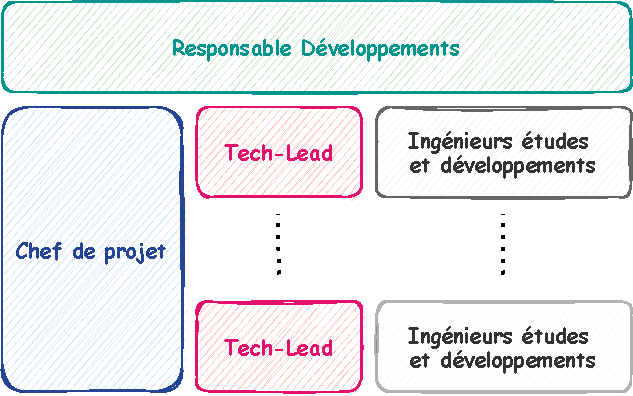
\includegraphics[width=\textwidth,]{images/sec3/organigrammedev.pdf}
        \caption{Organisation cible dév}
        \label{fig:subfig1}
    \end{subfigure}
    \hfill
    \begin{subfigure}[t]{0.39\textwidth}
        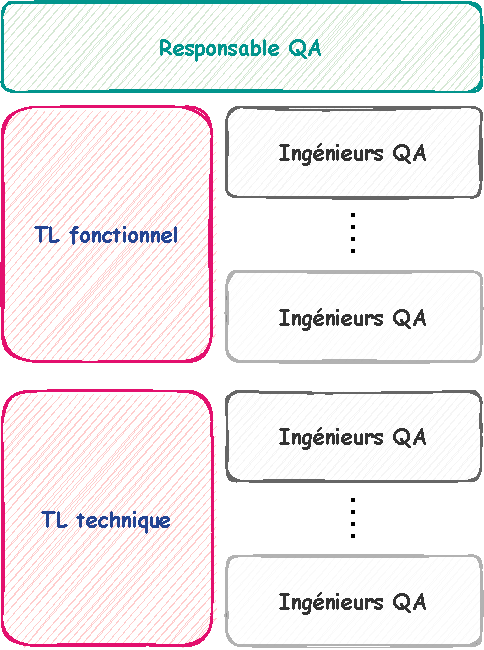
\includegraphics[width=\textwidth]{images/sec3/organigrammeqa.pdf}
        \caption{Organisation cible QA}
        \label{fig:subfig2}
    \end{subfigure}
    \caption{Modèle organisationnel visé pour les équipes de développement et de QA}
    \label{fig:devetqa}
\end{figure}
Le tableau suivant (\ref{tab:dev}) décrit les différentes activités et tâches confiées aux membres de l'équipe de développement impliqués dans le processus de livraison :
\begin{longtblr}[caption={Responsabilités et missions des différents acteurs de l'équipe de dév}, label={tab:dev}]{
    hlines = {0.25pt,azure6},
    vlines = {0.25pt,azure6},
    colsep=4pt,
    rowsep=4pt,
	colspec={X},
}
\textbf{Équipe de développement}
\\
\begin{minipage}{\linewidth}
{ \color{actGreen}
\textbf{Responsable Développements}\\
}
 \begin{itemize}
    \item Accompagner le chef de projet dans la gestion des projets.
    \item Produire des indicateurs sur l’activité de développement.
    \item Suivi des risques et gestion des alertes.
    \item Travailler en collaboration avec les autres responsables de division.\\
 \end{itemize}
\end{minipage}
\\
\begin{minipage}{\linewidth}
    {
        \color{actBlue}\textbf{Chef de projet}\\
    }
    \begin{itemize}
        \item Valider les spécifications fonctionnelles.
        \item Assurer le suivi du processus de livraison et des indicateurs clés.
        \item Élaboration du plan de charge et planification des équipes.
        \item Garant des engagements (Qualité, Délai, Coût).\\
    \end{itemize}
\end{minipage}\\
\begin{minipage}{\linewidth}
    {
        \color{actPink}\textbf{Tech-Lead}\\
    }
    \begin{itemize}
        \item Responsable de la qualité technique (Audit, conception, etc.).
        \item Responsable des bonnes pratiques de développement.
        \item Encadrement et assistance technique.
        \item Participer aux développements.
        \item Assister le chef de projet pour les estimations de charge.\\
    \end{itemize}
\end{minipage}\\
\begin{minipage}{\linewidth}
    {
        \textbf{Ingénieur étude et développement}\\
    }
    \begin{itemize}
        \item Corriger les anomalies et développer de nouveaux modules.
        \item Respecter les bonnes pratiques de développement.
        \item Participer à la définition de la couverture de tests techniques.
        \item Rédiger des documents techniques.\\
    \end{itemize}
\end{minipage}
\end{longtblr}
Le tableau suivant (\ref{tab:qa}) décrit les différentes activités et tâches assignées aux membres de l'équipe d'assurance qualité (QA) participant au processus de livraison :
\begin{longtblr}[caption={Responsabilités et missions des différents acteurs de l'équipe QA}, label={tab:qa}]{
    hlines = {0.25pt,azure6},
    vlines = {0.25pt,azure6},
    colsep=4pt,
    rowsep=4pt,
	colspec={X},
}
\textbf{Équipe QA}\\

\begin{minipage}{\linewidth}
{\color{actGreen}
\textbf{Responsable QA}\\
}
 \begin{itemize}
     \item Établir et piloter une stratégie de test.
     \item Accompagner le Team Lead dans la gestion des projets.
     \item Contribuer à l'amélioration des processus de test.
     \item Produire des indicateurs sur l’activité de testing.
     \item Suivi des risques et gestion des alertes.
     \item Travailler en collaboration avec les autres responsables de division.\\
 \end{itemize}
\end{minipage}\\
\begin{minipage}{\linewidth}
    {
    \color{actBlue}\textbf{TL fonctionnel/technique}\\
    }
    \begin{itemize}
        \item Responsable du suivi du processus de livraison et des indicateurs clés.
        \item Élaboration du plan de charge et la planification des équipes.
        \item Accompagner et suivre les testeurs dans la mise en place des bonnes pratiques et des outils.
        \item Accompagner les ingénieurs QA dans l'élaboration des plans de test.
        \item Réaliser le bilan des activités.
        \item Accompagner l'intégration des nouveaux arrivants et veiller à la montée en compétence des équipes.
        \item Participer aux activités de test.\\
    \end{itemize}
    \end{minipage}\\
    \begin{minipage}{\linewidth}
    {
        \textbf{Ingénieur QA}\\
    }
    \begin{itemize}
        \item Formaliser des scénarios de test fonctionnels et automatisés.
        \item Valider et vérifier le développement de l’application.
        \item Respecter les bonnes pratiques de testing.
        \item Rédiger des documents fonctionnels.\\
    \end{itemize}
\end{minipage}
\end{longtblr}

\subsubsection{Déroulement de projets - Méthode SCRUM}
Depuis 2019, les projets de R\&D ont progressivement passés en mode Agile. Ils utilisent la partie Agile de JIRA (catégorie Software).
Le mode Agile permet de gérer les projets en mode Scrum ou Kanban. Pour l'instant, Cegedim SRH utilise le mode Scrum.
\subsubsubsection{L'équipe Agile}
L'équipe Agile est une équipe qui entend être totalement autonome. Elle rassemble toutes les compétences nécessaires pour faire évoluer le produit. Le maître mot d'une équipe agile est la coopération. En effet, les membres de l'équipe ne travaillent pas séparément sur les fonctionnalités qui leur sont assignées, mais ensemble, y compris pour l'identification, la définition, la réalisation et les tests des fonctionnalités.

Les capacités d’écoute et d’entraide de l’équipe facilitent la montée en compétence. Chaque membre devient petit à petit plus ou moins polyvalent et en capacité d'aider les autres dans la réalisation des différentes fonctionnalités. L’équipe devient donc de plus en plus performante et efficace, tout en améliorant également le ressenti et les conditions de travail de chacun.
\begin{beware}
Une équipe Agile est en perpétuelle progression et évolution.
\end{beware}
Il n'y a pas de composition type pour une équipe Agile. Celle-ci dépend totalement du produit à réaliser. Certains rôles clefs sont néanmoins nécessaires au bon fonctionnement de l'équipe.
 La composition d'une équipe Agile au sein de la R\&D SRH suivra à minima le modèle suivant :

\begin{itemize}
\item \textbf{Equipe Agile R\&D}
\begin{itemize}
    \item 1 Product Owner ;
    \item 1 Scrum Master (optionnel mais conseillé) ;
    \item X développeurs (il est recommandé d'avoir +2) ;
    \item 1 QA (optionnel) ;
    \item X testeur(s)
\end{itemize}
\end{itemize}
Bien entendu, selon les produits, cette structure sera susceptible d'évoluer.
\subsubsubsection{Le Sprint}
Le Sprint agile est le cœur de la méthode SCRUM. Tous les développements sont réalisés de manière incrémentale au sein des Sprints. Un périmètre de développement - l'objectif du Sprint - est défini au début du Sprint lors du \textbf{Sprint Planning} avec la liste des \textbf{User Stories} à traiter pendant le Sprint.\\

À la conclusion d'un Sprint, le bilan est réalisé lors du \textbf{Sprint Review}, puis un nouveau cycle démarre avec un nouveau Sprint. La périodicité d'un Sprint dépendra de l'équipe Agile, mais sera généralement entre 2 et 4 semaines.

\subsubsubsection{Les Rituels}
Les rituels (ou cérémonies) sont des réunions de travail et de suivi qui viennent rythmer un Sprint. Chaque réunion joue un rôle précis dans le Sprint et correspond à une temporalité particulière.
\begin{itemize}
    \item \textbf{\underline{Sprint Planning}} : Le Sprint Planning est la réunion de lancement d'un Sprint. Au début de chaque Sprint, le Product Owner présente les User Stories qu'il souhaiterait intégrer au Sprint. Les User Stories sont examinées une par une dans l'ordre de priorité du Backlog jusqu'à ce que le Sprint soit complet en termes de vélocité.\\
    L'examen d'une User Story suit les étapes suivantes :
\begin{itemize}
    \item Lecture de la User Story par le Product Owner.
    \item Questions des développeurs (optionnel).
    \item Poker Planning : les développeurs estiment le temps nécessaire pour le développement de la User Story en votant chacun pour une durée. Pour passer à l'étape suivante, il doit y avoir un consensus sur l'estimation. Si tel n'est pas le cas, les développeurs ayant donné les estimations extrêmes doivent s'expliquer et un nouveau vote est réalisé.
    \item Intégration de la User Story au Sprint : passage en "A faire" dans le Board de l'équipe.
\end{itemize}
\begin{beware}[borderline west={5pt}{0pt}{olive3}, coltitle={olive3}, title=Note : ]
    Le Sprint Planning a lieu impérativement le premier jour du Sprint, de préférence le matin afin d'optimiser un maximum le temps de travail de l'équipe sur le Sprint.
\end{beware}
\begin{beware}[title=Remarque : ]
À l'étape "Questions", si les développeurs ne comprennent pas ce qu'il faut faire, la User Story est replacée dans le Backlog en vue d'être détaillée plus avant par le Product Owner.
De même, lors du "Poker Planning", si ces derniers n'arrivent pas à se mettre d'accord sur une estimation de temps commune.
\end{beware}

\item \textbf{\underline{Daily Stand-Up Meeting}} : Le Daily Stand-up meeting est une réunion quotidienne très courte (entre 5 et 15 minutes) à heure et lieu fixes qui rassemble l'ensemble des membres de l'équipe Agile où chaque membre de l'équipe prend la parole à tour de rôle. Chacun doit expliquer ce qu'il a fait depuis l'itération précédente du Stand-up meeting ou le Sprint Planning et ce qu'il prévoit faire jusqu'au prochain Stand-up meeting. 
\begin{beware}[borderline west={5pt}{0pt}{red}, coltitle={red}, title=Remarque : ]
Le temps de parole de chacun ne doit généralement pas dépasser deux minutes.
\end{beware}
Le Stand-up meeting a pour but de favoriser la circulation des informations au sein de l'équipe. Elle permet à l'ensemble de l'équipe d'avoir une vue complète de l'avancée des tâches et d'identifier d'éventuels points de blocages. Ces échanges dynamiques contribuent également à la cohésion et l'implication de l'équipe.
\begin{beware}[borderline west={5pt}{0pt}{red}, coltitle={red}, title=Attention : ]
\begin{itemize}
    \item La tenue du Stand-up meeting n'est pas facultative.
    \item Si un sujet est susceptible de déborder, il doit être traité en dehors du cadre du Stand-up meeting avec les membres concernés.
\end{itemize}
\end{beware}
\item \textbf{\underline{Sprint Retrospective}} : La Sprint Retrospective est la réunion d'analyse du déroulement du Sprint par l'équipe. Elle est positionnée à la fin de chaque sprint, après le Sprint Review. L'idée pour l'équipe est de capitaliser sur le vécu du Sprint écoulé pour adapter son organisation dans le but de renforcer son efficacité. C'est un élément clef dans le processus de progression et d'apprentissage de l'équipe.

L'équipe doit définir un plan d'action et d'amélioration à partir des constats et idées remontés pendant la réunion.

\item \textbf{\underline{Sprint Review}} :
Le Sprint Review est une réunion qui se situe en toute fin d'un Sprint juste avant le Sprint Retrospective.
Elle a pour but de présenter le travail réalisé durant le Sprint courant.
Le but est d'obtenir un maximum de retours sur le réalisé afin d'assurer qu'il est bien en accord avec les attentes.

Si l'avancée le permet, elle s’agrémente généralement en fin de Sprint Review d'une démonstration des nouveautés. 
Si tel n'est pas le cas, la démonstration peut être effectuer séparément du Sprint Review.
\begin{beware}[borderline west={5pt}{0pt}{olive3}, coltitle={olive3}, title=Note : ]
   Cette réunion inclut non seulement l'équipe Agile mais aussi les parties prenantes et les décideurs.
\end{beware}
\end{itemize}


\subsubsection{Processus de développement}
Compte tenu de la diversité des applications développées par Cegedim SRH et afin de mener à bien la mise en place des solutions, cette dernière adopte un processus de développement où tout projet est amené à suivre. Je ne ferai référence dans cette partie que sur un périmètre limité de ce processus, et sur lequel je suis intervenu à collaborer et échanger.
\begin{itemize}
    \item \textbf{\underline{Analyse fonctionnelle et définition des objectifs}} : Lors de cette phase préalable au démarrage du projet, les parties prenantes définissent ensemble :
    \begin{itemize}
        \item les objectifs et la portée du projet,
        \item les livrables attendus,
        \item les délais souhaités,
        \item le degré de souplesse qui pourra être accordé.
    \end{itemize}
    \item \textbf{\underline{Étude de faisabilité et formalisation des spécifications techniques}} : Une étude de faisabilité peut être menée afin de cerner les contraintes susceptibles de peser sur la mise en œuvre du projet. Ensuite, les spécifications techniques sont formalisées, faisant état des méthodes, processus et technologies qui seront utilisés pour répondre aux contraintes du projet.
    \item \textbf{\underline{Découpage et chiffrage}} : Il s'agit d'établir la liste des tâches en associant les besoins et les coûts correspondants, tout en incluant les sous-tâches et les tâches induites par la réalisation afin de chiffrer au plus juste le projet.
    \item \textbf{\underline{Planification}} : La planification vise à ordonner les tâches et à indiquer leur enchaînement logique en tenant compte des ressources disponibles et de leur charge de travail maximale.
    \item \textbf{\underline{Codage}} : La phase de codage, également appelée programmation, consiste à traduire en code les fonctionnalités et les exigences techniques préalablement définies.
    \item \textbf{\underline{Tests unitaires}} : Le concept de test unitaire n'est pas un élément nouveau. Depuis les prémices de l'informatique, les tests font partie de l'activité quotidienne d'un développeur. Ce qui est nouveau aujourd'hui, c'est que cette activité, notamment les tests unitaires, est placée au cœur du processus de conception. En effet, un test unitaire permet de valider la conformité de chaque composant logiciel pris comme une unité par rapport à sa spécification détaillée. Autrement dit, un scénario de test unitaire ressemble à une expérience scientifique dans laquelle une hypothèse est examinée en fonction de trois éléments clés :
    \begin{enumerate}
        \item Les données en entrée. 
        \item L'objet à tester. 
        \item Les observations attendues.
    \end{enumerate}
    \item \textbf{\underline{Audit de code}} : L'étape d'audit de code permet de s'assurer de la qualité du codage en vérifiant que chaque module ou sous-ensemble de la solution informatique est conforme aux règles et bonnes pratiques de développement logiciel. Dans le cadre de ce sujet, nous nous référerons plus particulièrement aux règles établies par Cegedim SRH (voir la checklist \ref{sec:checklist} en annexe) dans le but de systématiser les bonnes pratiques et d'éviter les erreurs classiques de développement au sein des équipes de dév.
    \item \textbf{\underline{Recette}} La phase de recette est le processus de validation par l'équipe de validation et acceptance (QA) de la conformité des livrables avec les spécifications initiales.
    \item \textbf{\underline{Documentation}} : À l’issue de la recette, une documentation de projet est produite afin de rassembler les informations nécessaires à l’utilisation de la solution informatique et en vue de ses développements ultérieurs.
    \item \textbf{\underline{Déploiement}} : Une fois le projet qualifié, la solution informatique peut être déployée : il s’agit de la livraison du produit final et de sa mise en service.
\end{itemize}
\subsubsection{Gestion du workflow git}
Le workflow de travail pour les branches GIT choisi au niveau de Cegedim SRH est Gitflow. Git Flow est un modèle de dépôt git permettant d'améliorer les processus de développement et de mise en production d'un projet.\\

Gitflow sépare sur des branches isolées le code en cours de développement et le code validé et testé. Pour cela, il s’appuie sur la création de plusieurs branches dont le cycle de vie est bien défini. Voici une table contenant leurs noms, leurs cycles de vie et leurs fonctions (voir la table \ref{tab:gitflow}):
\begin{longtblr}[caption={Présentation des différentes branches définies sur gitflow},label={tab:gitflow}]{
        hlines = {0.25pt,azure6},
        vlines = {0.25pt,azure6},
        row{1} = {bg=azure9!10!white},
        colsep=4pt,
        rowsep=4pt,
    	colspec={Q[2]Q[2]Q[2]Q[3]X[8]},
        rowspec={Q[m] Q[m] Q[m] Q[m] Q[m] Q[m] Q[m]},
    }
    \textbf{Branche}&\textbf{Nombre}&\textbf{Branche d’origine}&\textbf{Durée de vie}&\textbf{Fonction}\\
    master & Unique & & Permanente & Code stable, testé et validé potentiellement éligible pour une MEP (Mise En Production)\\
    feature & Plusieurs & develop & Développement d'une fonctionnalité & Code en cours de développement destiné à réaliser une fonctionnalité à intégrer dans la prochaine version de l'application.\\
    develop & Unique & master & Permanente & Code de la prochaine version de l’application. Une fois que le développement d’une fonctionnalité (feature) est fini, le code est fusionné sur cette branche.\\
    release & Unique & develop & Recette & Branche sur laquelle on corrigera les bugs détectés pendant la phase de recette.\\
    hotfix & Aucune / Plusieurs & master & Correction d’un bug & Branche où on fait les corrections des bugs sur le code présent sur la branche master (production).
\end{longtblr}
Voici un schéma présentant l'organisation du dépôt git ainsi que les différentes interactions qu'il peut y avoir entre chaque branche (voir la figure \ref{fig:gitflow}) :
\begin{figure}[H]
    \begin{center}
        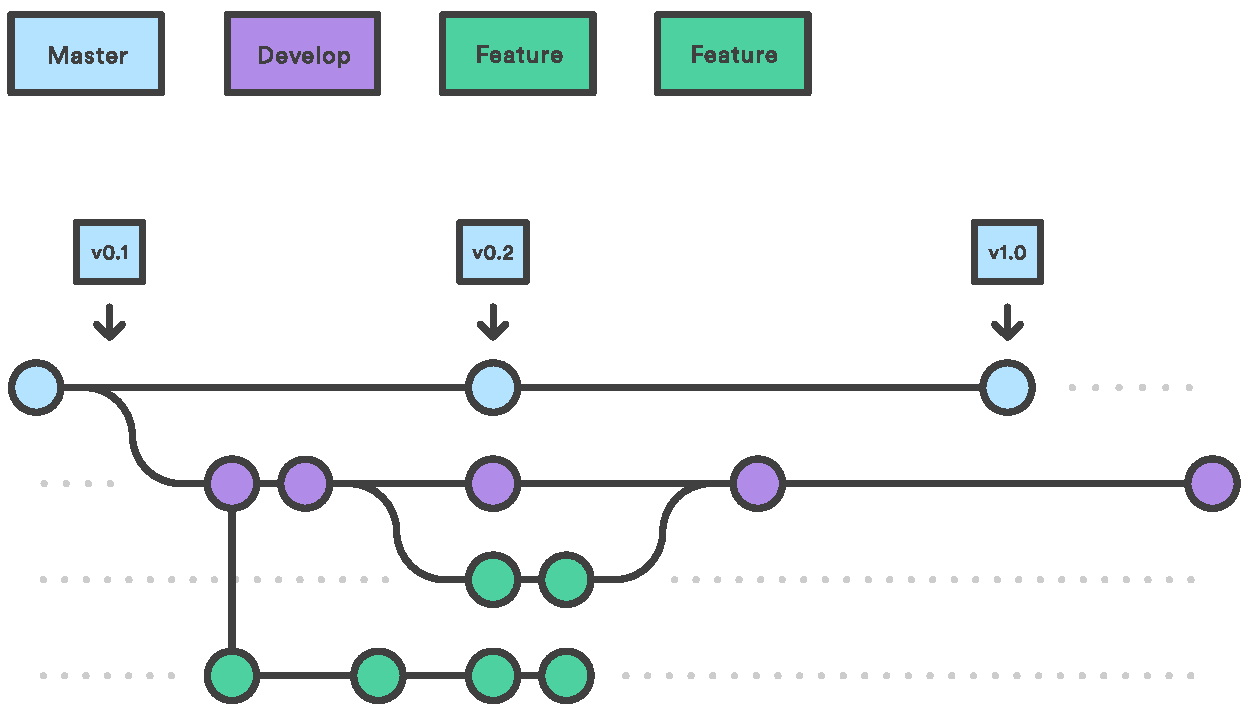
\includegraphics[width=0.8\linewidth]{images/sec3/gitflow.pdf}
        \caption{Schéma illustrant l'interaction entre les différentes branches du flux de travail gitflow}
        \label{fig:gitflow}
    \end{center}
\end{figure}
\subsection{Planification et suivi du projet}
La planification est parmi les phases d'avant-projet. Elle consiste non seulement à délimiter le périmètre temporel du projet, mais aussi à prévoir le déroulement des activités tout au long de la période allouée au stage.

\subsubsection{Diagramme de Gantt}
La figure suivante détaille la planification prévisionnelle du projet (voir figure \ref{fig:gantt}):\\
\begin{figure}[H]
    \begin{center}
        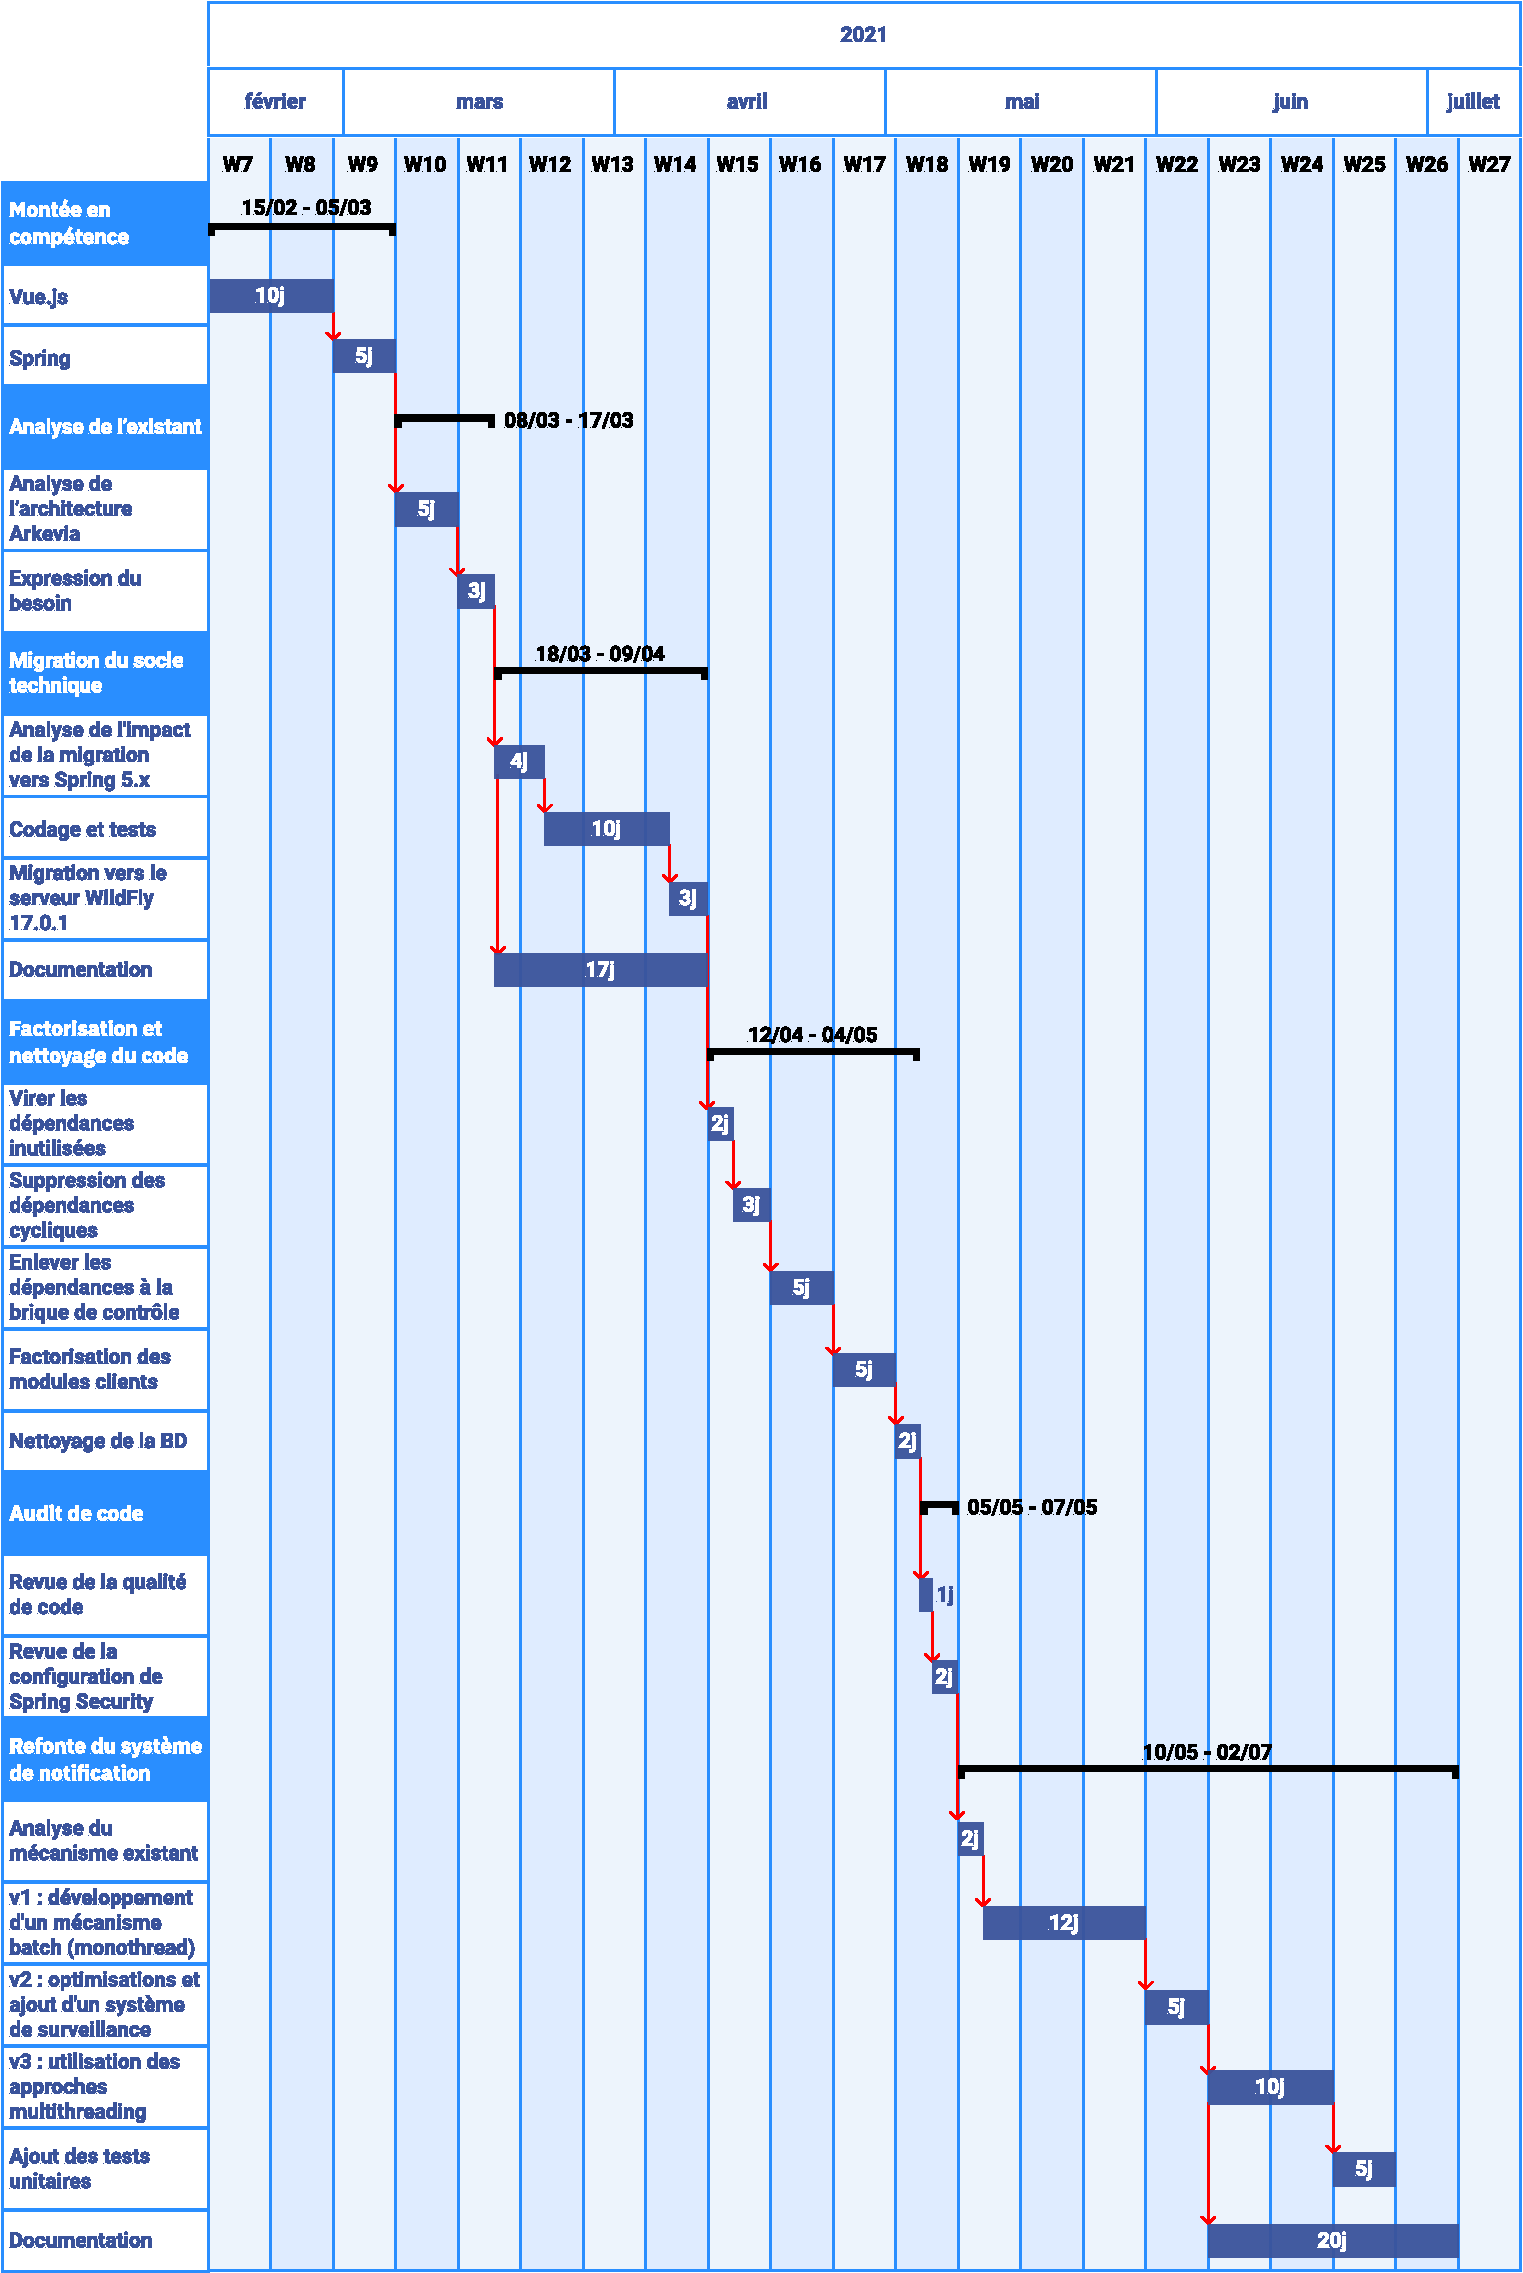
\includegraphics[width=\linewidth]{images/sec3/gantt.pdf}
        \caption{Diagramme de Gantt}
        \label{fig:gantt}
    \end{center}
\end{figure}

\subsection*{Conclusion}
\addcontentsline{toc}{subsection}{Conclusion}
La gestion de projets comme l’on peut le constater s’avère être d’une grande nécessité. Il est nécessaire pour mener à bien un projet de prendre en compte plusieurs dimensions dont toutes ne sont pas forcément quantifiables.\\

Cegedim SRH adopte désormais la méthode Scrum, l'une des méthodes Agile les plus répandues, pour le développement de ses propres solutions. L'Agilité, résolument basée sur l'efficacité et la création de valeur ajoutée, place véritablement clients et éditeurs dans un mode collaboratif avec comme vision un objectif commun.\\

En conséquence, grâce à son expertise avérée de cette méthodologie. Cegedim SRH a pu réduire les délais de conception et de production sans pour autant compromettre la qualité du produit final.
%%%%%%%%%%%%%%%%%%

% %%%%%%%%%%%%%%%%%%%%%%%%%%%%%%%%%%%%%%%%%%%%%%%%%%%
%% Conceptions et spécification des besoins
%%%%%%%%%%%%%%%%%%%%%%%%%%%%%%%%%%%%%%%%%%%%%%%%%%%
\section{Conceptions et spécification des besoins}
\addcontentsline{toc}{subsection}{Introduction}
\subsection*{Introduction}
Ce chapitre est voué à fournir une conception détaillée du portail Arkevia (le portail existant), afin d'appréhender son mode de fonctionnement et de bien cerner les besoins et exigences liés au sujet. Nous poursuivons cette conception par l'élaboration des besoins, des contraintes, et des méthodologies et solutions préconisées.
\subsection{Étude conceptuelle du système existant}
L'objectif de cette première section est de mener une étude conceptuelle approfondie du fonctionnement du système.
\subsubsection{Méthodologie de conception}
L’utilisation de la modélisation conceptuelle dans le développement des systèmes d’information permet de prendre en compte les besoins des applications d’une façon plus adéquate et de présenter d’une manière abstraite certains aspects des systèmes physiques et humains.\\

Afin de modéliser et décrire les différents aspects de notre système, nous utiliserons le langage graphique de modélisation unifié UML 2.0.\\
UML est un langage formel et normalisé en termes de modélisation objet. Son indépendance par rapport aux langages de programmation, aux domaines d’application et son caractère polyvalent ont fait de lui un langage universel. Il fournit un moyen astucieux permettant de représenter diverses projections, grâce aux diagrammes.\\
% Les diagrammes sont représentés sous deux types de vue :
% \begin{itemize}
%     \item D'un point de vue \textbf{statique} ou \textbf{structurelle} du domaine avec les diagrammes de structure (Structure Diagrams).
%     \item D'un point de vue \textbf{dynamique} avec les diagrammes de comportement (Behavior Diagrams) et les diagrammes d’interactions (Interaction Diagrams).\\
% \end{itemize}

% L’utilisation itérative des outils UML dans l’analyse et la conception, permet d’obtenir une meilleure compréhension de la configuration système requise et les processus à exécuter dans le système pour répondre à ces exigences.\\
% La première itération d’analyse devrait se situer à un niveau très élevé afin de déterminer les objectifs généraux du système et de valider les exigences au moyen d’une analyse du cas d’utilisation. L’identification des acteurs et la définition du modèle de cas d’utilisation initial font partie de cette première itération. Les itérations d’analyse ultérieures affinent davantage la configuration système requise en développant des scénarios de cas d’utilisation, des diagrammes de classes, des diagrammes de séquence, des diagrammes d’états, etc. Chaque itération prend successivement plus en détail la conception du système jusqu’à ce que les objets et les relations dans le système soient clairement et précisément définis dans les diagrammes UML.\\

% Une fois l'analyse terminée, nous aurons une vue complète, détaillée et précise de l'ensemble des spécifications des classes, des scénarios, des activités et de leur enchaînement dans le système. En général, on peut établir des liens entre la rigueur de l'analyse et de la conception d'un système, le temps nécessaire pour effectuer les développements et la qualité du produit livré en conséquence.
% \\
% \begin{beware}[title=Conclusion : ]
%     L'UML propose des diagrammes pour décrire les différents aspects de l'application, mais ne précise pas la séquence des étapes à suivre ni la démarche à suivre pour la mise en œuvre de ces diagrammes. Un processus de livraison est alors nécessaire (voir section \ref{sec:delivery}).
% \end{beware}

\subsubsection{Identification des acteurs}
Un acteur représente un rôle, c'est-à-dire une personne, un matériel ou un logiciel qui interagit directement avec le système. Les acteurs pouvant interagir avec l’application sont :
\begin{itemize}
    \item \textbf{Employeur} : Personne morale adressant aux utilisateurs des documents.
    \item \textbf{Titulaire} : Salarié, actuel ou passé, de l’Employeur ayant ouvert et utilisant le coffre-fort électronique.
    \item \textbf{Utilisateur} : Titulaire ou, le cas échéant, les personnes physiques spécifiquement habilitées par le Titulaire.
    \item \textbf{Opérateur} : Personne morale qui met en œuvre un service de coffre-fort électronique et règle le fonctionnement opérationnel du système et des mesures de sécurité afférentes, en l’espèce CEGEDIM SRH. 
\end{itemize}

\subsubsection{Diagramme de cas d'utilisation général}
Le diagramme de cas d'utilisation représente la structure des grandes fonctionnalités nécessaires aux utilisateurs du système. C'est le premier diagramme du modèle UML, celui où s'assure la relation entre l'utilisateur et les objets que le système met en œuvre.\\
Un cas d'utilisation est une description de l'application qui privilégie le point de vue de l'utilisateur. Il décrit de façon graphique (ou éventuellement textuelle) comment un acteur va utiliser l'application pour atteindre un objectif.
\begin{figure}[H]
    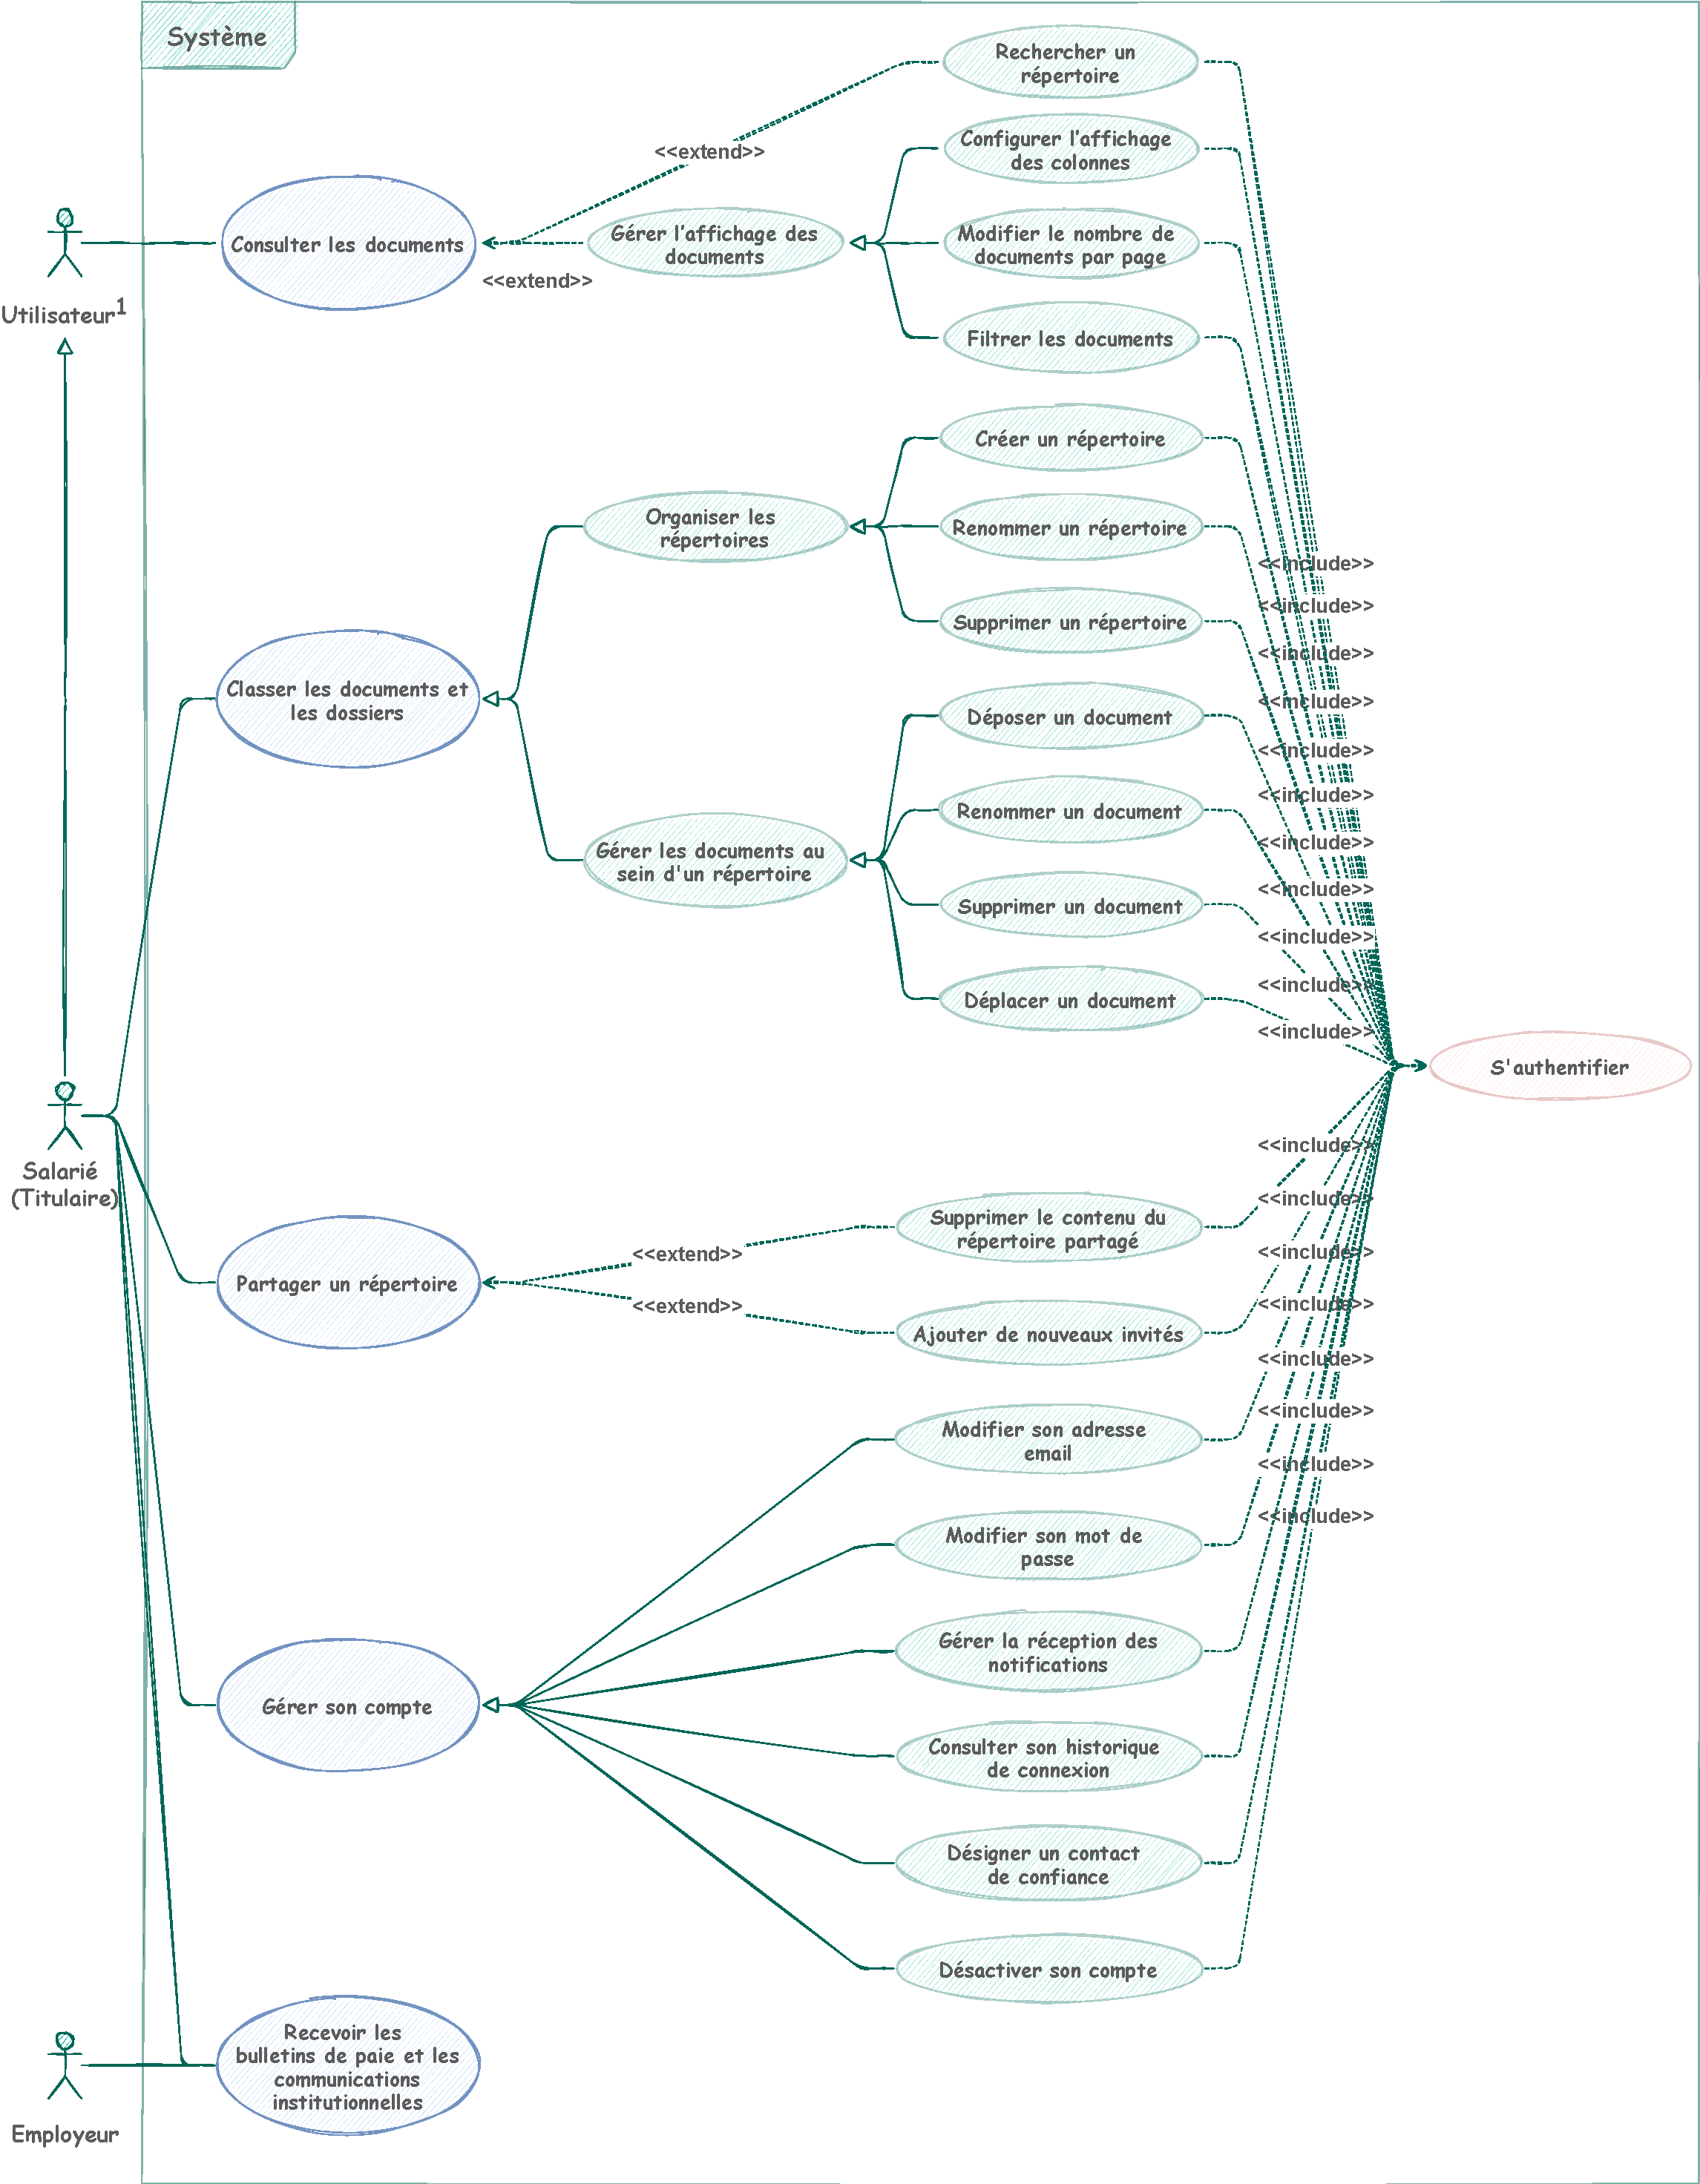
\includegraphics[width=1.1\linewidth]{images/sec3/usecase.pdf}
    \caption{Diagramme de cas d'utilisation général}
    \label{fig:uc}
\end{figure}
\footnotetext[1]{représente le cas d'un acteur (non propriétaire) autorisé à utiliser le compte.}
\hfill
\vspace{-1.5cm}
\subsubsection{Raffinement des cas d'utilisation prioritaires}
\subsubsubsection*{Cas d’utilisation : « S'inscrire »}
\setlength{\fboxrule}{1pt}
\setlength{\fboxsep}{6pt}
\begin{longtblr}[caption={Description textuelle du CU « S'inscrire »},
    note{1} = {Le mot de passe doit comporter un minimum de 8 caractères et un maximum de 20 caractères, au moins une lettre, au moins un chiffre, au moins un caractère spécial parmi @\#\$\%\^\&+=?\_|!,;.:\/ et ne doit pas contenir d'espaces.}]{
    hlines = {0.5pt,chambray},
    vlines = {0.5pt,chambray},
    colsep=4pt,
    rowsep=4pt,
    colspec={Q[l]X[l]},
    rowspec={Q[m] Q[m] Q[m] Q[m] Q[m] Q[m]},
}
\textbf{Acteur} & Salarié (Titulaire) \\
\textbf{Objectif}& 
L'inscription permet aux salariés d'activer la mise à disposition de leurs bulletins de paie électroniques dans leurs coffres-forts.\\
\textbf{Pré-condition} & 
Disposer d'une connexion Internet et d'un navigateur.\\
\textbf{Scénario} & 
\begin{minipage}{\linewidth}
\raggedright
\begin{enumerate}[leftmargin=*]
    \item Le salarié se rend sur \url{www.myarkevia.com} à l'aide d'un navigateur.
    \item Le salarié clique sur \fcolorbox{arkevia-btn-border}{arkevia-btn-bg}{\textcolor{white}{\scriptsize\textbf{JE M'INSCRIS}}}.
    \item Le salarié renseigne le matricule et le code secret qui lui ont été communiqués par le service RH, soit par des courriers spécifiques, soit par son dernier bulletin de salaire papier.
    \item Le salarié doit tenir compte de la \textbf{convention de mise à disposition du bulletin de paie électronique par l’employeur} et cocher la case \textcolor{gray}{\faCheckSquare\ J’ai lu et j’accepte les conditions de la convention} pour pouvoir passer à l’étape suivante.
    \item Le salarié renseigne les champs obligatoires concernant son profil.
   \item Le salarié doit tenir compte des \textbf{Conditions Générales d’Utilisation} et cocher la  case \textcolor{gray}{\faCheckSquare\ J’accepte les conditions générales d’utilisation d’ARKEVIA} pour pouvoir passer à l’étape suivante.
   \item Le salarié saisit son mot de passe conformément aux règles de sécurité\TblrNote{1}, puis le confirme.
   \item Enfin, le salarié clique sur \fcolorbox{arkevia-btn-border}{arkevia-btn-bg}{\textcolor{white}{\scriptsize\textbf{VALIDER MON INSCRIPTION}}} pour confirmer son inscription.
\end{enumerate}
\end{minipage}
\\
\textbf{Exception} & \begin{minipage}{\linewidth}
\raggedright
\begin{itemize}[leftmargin=*]
    \item Ouvert aux seuls salariés des entreprises ayant conclues un contrat de services avec CEGEDIM SRH (« Service ARKEVIA »)
    \item Le salarié saisit un matricule ou un code secret invalide.
    \item Le salarié saisit un mot de passe non conforme aux règles de sécurité définies par le système.
\end{itemize}
\end{minipage}
\\
\textbf{Post-condition} & Le système redirige automatiquement le salarié vers la page de connexion.\\
\end{longtblr}
\hfill
\vspace{-1.4cm}
\subsubsubsection*{Cas d’utilisation : « Se connecter »}
\begin{longtblr}[caption={Description textuelle du CU « Se connecter »}]{
    hlines = {0.5pt,chambray},
    vlines = {0.5pt,chambray},
    colsep=4pt,
    rowsep=4pt,
    colspec={Q[l]X[l]},
    rowspec={Q[m] Q[m] Q[m] Q[m] Q[m] Q[m]},
}
\textbf{Acteur} & Salarié, actuel ou passé, ayant ouvert et utilisant le coffre-fort électronique, et le cas échéant, les personnes physiques spécifiquement habilitées par le titulaire. \\
\textbf{Pré-condition} & 
\begin{minipage}{\linewidth}
\raggedright
\begin{itemize}[leftmargin=*]
    \item Avoir préalablement suivi la procédure d'inscription.
    \item Disposer d'une connexion Internet et d'un navigateur.
\end{itemize}
\end{minipage}
\\
\textbf{Scénario} & 
\begin{minipage}{\linewidth}
\raggedright
\begin{enumerate}[leftmargin=*]
    \item L'utilisateur se rend sur \url{www.myarkevia.com} à l'aide d'un navigateur.
    \item L'utilisateur saisit son adresse e-mail et son mot de passe.
    \begin{itemize}
        \item Si nécessaire, il peut cliquer sur l’oeil \faEye{ } dans le champ \textbf{Mot de passe} pour voir son mot de passe en toutes lettres et ainsi éviter des erreurs de saisie.
    \end{itemize}
   \item Le salarié clique sur \fcolorbox{arkevia-btn-border}{arkevia-btn-bg}{\textcolor{white}{\scriptsize\textbf{JE ME CONNECTE}}} pour confirmer son inscription.
\end{enumerate}
\end{minipage}
\\
\textbf{Exception} & \begin{minipage}{\linewidth}
\raggedright
\begin{itemize}[leftmargin=*]
    \item Le salarié entre un mot de passe ou un e-mail incorrect.
    \item Au-delà de trois tentatives erronées, le système suspecte un abus ou une utilisation illégale de la part de l'utilisateur et bloque donc l'accès au compte pour une période de 15 minutes.
\end{itemize}
\end{minipage}
\\
\textbf{Post-condition} & Le système redirige l'utilisateur vers la page d'accueil de son compte.\\
\end{longtblr}

\subsubsubsection*{Cas d’utilisation : « Créer un nouveau répertoire »}
\begin{longtblr}[caption={Description textuelle du CU « Créer un nouveau répertoire »}, note{2} = {Les noms de répertoire ne peuvent pas contenir d'espaces, ni de caractères non conformes aux règles de nommage des fichiers Unix.}]{
    hlines = {0.5pt,chambray},
    vlines = {0.5pt,chambray},
    colsep=4pt,
    rowsep=4pt,
    colspec={Q[l]X[l]},
    rowspec={Q[m] Q[m] Q[m] Q[m] Q[m] Q[m]},
}
\textbf{Acteur} & Salarié (Titulaire) \\
\textbf{Objectif}& 
Permettre au salarié de créer ses propres répertoires afin de stocker et classer ses documents (bulletins de paie ou documents personnels qu'il a déposés dans son coffre-fort).\\
\textbf{Pré-condition} & 
S'authentifier avec un identifiant correct.\\
\textbf{Scénario} & 
\begin{minipage}{\linewidth}
\raggedright
\begin{enumerate}[leftmargin=*]
    \item Dans la section répertoire de l'écran, le salarié sélectionne le dossier sous lequel il souhaite créer un répertoire. Le dossier sélectionné est alors marqué en vert.
    \item Le salarié clique sur l’icône \faPlusSquareO { }\textbf{Créer un nouveau répertoire}.
    \item Le salarié renseigne le nom du nouveau répertoire.
   \item Le salarié clique sur \fcolorbox{arkevia-btn-bg}{arkevia-btn-bg}{\textcolor{white}{\scriptsize\textbf{Créer}}}.
\end{enumerate}
\end{minipage}
\\
\textbf{Exception} & \begin{minipage}{\linewidth}
\raggedright
\begin{itemize}[leftmargin=*]
    \item Le nom du répertoire est invalide\TblrNote{2}.
    \item Création d'un répertoire avec un nom qui existe déjà.
\end{itemize}
\end{minipage}
\\
\textbf{Post-condition} & Le système renvoie un message indiquant à l'utilisateur qu'il peut désormais déposer des fichiers dans son nouveau répertoire.\\
\end{longtblr}


\subsubsubsection*{Cas d’utilisation : « Déposer un document »}
\begin{longtblr}[caption={Description textuelle du CU « Déposer un document »}]{
    hlines = {0.5pt,chambray},
    vlines = {0.5pt,chambray},
    colsep=4pt,
    rowsep=4pt,
    colspec={Q[l]X[l]},
    rowspec={Q[m] Q[m] Q[m] Q[m] Q[m] Q[m]},
}
\textbf{Acteur} & Salarié (Titulaire) \\
\textbf{Objectif}& 
Permettre aux salariés d'importer leurs documents importants.\\
\textbf{Pré-condition} & 
S'authentifier avec un identifiant correct.\\
\textbf{Scénario} & 
\begin{minipage}{\linewidth}
\raggedright
\begin{enumerate}[leftmargin=*]
    \item Le salarié sélectionne un dossier sous lequel il souhaite importer ses documents.
    \item Le salarié clique sur \fcolorbox{white}{arkevia-btn-bg2}{\textcolor{white}{ \scriptsize\textbf{\faFileO { } Déposer un document}}}.
   \item Dans la fenêtre \textbf{Ajout d’un document}, le salarié clique sur \fcolorbox{gray6}{gray!20!white}{\scriptsize\textbf{Choisir un fichier}}.
   \item Le salarié parcourt ses répertoires et sélectionne un fichier. Il peut éventuellement sélectionner plusieurs fichiers en appuyant sur la touche Ctrl et en cliquant simultanément avec la souris sur les fichiers souhaités.
    \item Le salarié clique sur \fcolorbox{arkevia-btn-bg}{arkevia-btn-bg}{\textcolor{white}{\scriptsize\textbf{Ajouter}}}.
\end{enumerate}
\end{minipage}
\\
\textbf{Exception} & 
Le fichier dépasse la taille limite autorisée de 50 Mo.\\
\textbf{Post-condition} & Le système renvoie un message indiquant à l'utilisateur que les documents sont en cours d'importation, puis un autre message indiquant le statut de l'opération lorsqu'elle est terminée.
\end{longtblr}

\subsubsubsection*{Cas d’utilisation : « Gérer un document »}
\begin{longtblr}[caption={Description textuelle du CU « Gérer un document »}]{
    hlines = {0.5pt,chambray},
    vlines = {0.5pt,chambray},
    colsep=4pt,
    rowsep=4pt,
    colspec={Q[l]X[l]},
    rowspec={Q[m] Q[m] Q[m] Q[m] Q[m] Q[m]},
}
\textbf{Acteur} & Salarié (Titulaire) \\
\textbf{Objectif}& 
Permettre aux salariés d'importer leurs documents importants.\\
\textbf{Pré-condition} & 
S'authentifier avec un identifiant correct.\\
\textbf{Scénario} & 
\begin{minipage}{\linewidth}
\raggedright
\begin{enumerate}[leftmargin=*]
    \item Le salarié sélectionne un répertoire pour accéder à son contenu.
    \item Dans la partie \textbf{Détail du répertoire} de l’écran, Il peut cliquer sur :
    \begin{itemize}
        \item L’icône \textcolor{gray7}{\textbf{Consulter} \faEye{ }} pour consulter le document.
        \item L’icône \textcolor{gray7}{\textbf{Renommer} \faPencil{ }} pour renommer le document.
        \item L’icône \textcolor{gray7}{\textbf{Supprimer} \faTrash{ }} pour supprimer le document.
        \item Le \textbf{nom du document} et, tout en maintenant le clic, il peut le glisser-déposer dans un répertoire de son choix.
    \end{itemize}
\end{enumerate}
\end{minipage}
\\
\textbf{Exception} & 
\begin{minipage}{\linewidth}
\raggedright
\begin{itemize}[leftmargin=*]
    \item Les documents professionnels déposés par l'employeur ne peuvent pas être supprimés par le salarié.
    \item Le nom du document ne peut pas être renommé avec un nom qui existe déjà dans le répertoire parent.
\end{itemize}
\end{minipage}
\\
\textbf{Post-condition} & 
Pour chaque action effectuée, le système renvoie un message indiquant à l'utilisateur l'état de l'opération lorsqu'elle est terminée.//
\end{longtblr}

\subsubsubsection*{Cas d’utilisation : « Gérer l'affichage des documents »}
\begin{longtblr}[caption={Description textuelle du CU « Gérer l'affichage des documents »}, , note{3} = {Les filtres actifs s’affichent au-dessus de la section \textbf{Détail du répertoire}.}]{
    hlines = {0.5pt,chambray},
    vlines = {0.5pt,chambray},    
    colsep=4pt,
    rowsep=4pt,
    colspec={Q[l]X[l]},
    rowspec={Q[m] Q[m] Q[m] Q[m] Q[m] Q[m]},
}
\textbf{Acteur} & Salarié (Titulaire) \\
\textbf{Objectif}& 
Permettre aux salariés de configurer l’affichage des colonnes du tableau \textbf{Détail du répertoire}, de filtrer les  documents ainsi que d'ajuster le nombre de documents affichés par page.
\\
\textbf{Pré-condition} & 
S'authentifier avec un identifiant correct.\\
\textbf{Scénario} & 
\begin{minipage}{\linewidth}
\raggedright
\begin{itemize}[leftmargin=*]
    \item Pour configurer l’affichage des colonnes : 
    \begin{enumerate}
        \item Le salarié sélectionne un répertoire pour en afficher le contenu dans le tableau \textbf{Détail du répertoire}.
        \item Le salarié clique sur la liste déroulante \textbf{Gérer les colonnes} et coche les colonnes qu'il souhaite afficher et décoche celles qu'il souhaite masquer.
    \end{enumerate}
    \item Si le répertoire contient un grand nombre de documents, ils sont alors affichés sur plusieurs pages que le salarié peut parcourir à l'aide des boutons situés sous le tableau. Pour plus de commodité, le salarié a la possibilité d'afficher plus de lignes dans le tableau et ainsi de réduire le nombre de pages. Pour ce faire :
    \begin{enumerate}
        \item Le salarié clique sur la liste déroulante \textbf{[X] lignes}.
        \item Le salarié sélectionne 5, 10 ou 20 lignes.
    \end{enumerate}
    \item Le salarié a également la possibilité de filtrer les documents pour n'afficher que ceux correspondant aux critères de sélection qu'il a choisis. Pour ce faire :
    \begin{enumerate}
        \item Le salarié clique sur le bouton \fcolorbox{arkevia-btn-bg}{arkevia-btn-bg}{\textcolor{white}{\scriptsize\textbf{Filtrer } \faSliders}}.
        \item Parmi les 5 filtres proposés, le salarié clique sur les filtres souhaités. 
        \item Dans le champ qui s’affiche, le salarié renseigne les critères de filtrage.
        \item Le salarié clique  sur \fcolorbox{arkevia-btn-bg}{arkevia-btn-bg}{\textcolor{white}{\scriptsize\textbf{Appliquer les filtres}}}\TblrNote{3}.
        \item Le salarié clique sur la croix \textcolor{gray}{\faClose} pour fermer le volet des filtres.
    \end{enumerate}
    \item Pour désactiver le filtrage :
    \begin{enumerate}
        \item Le salarié clique sur le bouton \fcolorbox{arkevia-btn-bg}{arkevia-btn-bg}{\textcolor{white}{\scriptsize\textbf{Filtrer } \faSliders}} pour afficher le volet des filtres.
        \item Pour désactiver tous les filtres, le salarié clique sur le bouton Annuler \fcolorbox{arkevia-btn-bg}{white}{\textcolor{gray}{\faRefresh}}.
        \item Le salarié peut également désactiver certains filtres en cliquant sur le filtre à désactiver puis sur la croix \fcolorbox{white}{arkevia-btn-bg}{\textcolor{white}{\faClose}} pour supprimer les critères saisis.
A la fin, l'employé clique sur Appliquer les filtres pour rafraîchir la liste des documents.
\item Le salarié clique sur la croix \textcolor{gray}{\faClose} pour fermer le volet des filtres.
    \end{enumerate}
\end{itemize}
\end{minipage}
\\
\textbf{Exception} & Aucune
\\
\textbf{Post-condition} & 
Pour chaque action effectuée, l’affichage est instantanément modifié.
\end{longtblr}
\break
\subsubsubsection*{Cas d’utilisation : « Gérer le partage des documents »}
\begin{longtblr}[caption={Description textuelle du CU « Partager un répertoire »},
note{4} = {La date saisie doit être postérieure à la date du jour.},
note{5} = {En ajoutant des documents au dossier  partagé, l'utilisateur crée simplement une copie des documents d'origine. Ils ne sont en aucun cas supprimés du répertoire d’origine.},
note{6} = {Il est impératif de cocher la case Envoyer une notification aux invités, sinon ils ne recevront pas de notification pour télécharger les documents qui leur sont partagés.}]{
    hlines = {0.5pt,chambray},
    vlines = {0.5pt,chambray},   
    colsep=4pt,
    rowsep=4pt,
    colspec={Q[l]X[l]},
    rowspec={Q[m] Q[m] Q[m] Q[m] Q[m] Q[m]},
}
\textbf{Acteur} & Salarié (Titulaire) \\
\textbf{Objectif}& 
Donnez aux salariés la possibilité de créer des répertoires de partage afin qu'ils puissent partager des documents avec des tiers en dehors de leur entreprise.\\
\textbf{Pré-condition} & 
S'authentifier avec un identifiant correct.\\
\textbf{Scénario} & 
\begin{minipage}{\linewidth}
\raggedright
\begin{enumerate}[leftmargin=*]
    \item Le salarié doit d'abord créer un répertoire partagé, cela peut être fait à travers le scénario suivant :
    \begin{enumerate}
        \item Dans la liste des répertoires, le salarié clique sur le dossier \textbf{Partage}.
        \item Le salarié clique sur l’icône \textbf{Ajouter un répertoire partagé} \faShareAltSquare.
        \item Dans la fenêtre \textbf{Nouveau partage}, le salarié renseigne les champs suivants :
        \begin{itemize}
            \item \textbf{Nom du répertoire}.
            \item \textbf{Liste des invités} : il saisit les adresses e-mail des personnes avec lesquelles il souhaite partager ses documents, séparées par une virgule.
            \item \textbf{Commentaire}.
            \item \textbf{Date d’expiration du partage} : il saisit la date\TblrNote{4} jusqu’à laquelle le tiers pourra accéder au contenu de son répertoire de partage.
        \end{itemize}
        \item Le salarié clique sur \fcolorbox{arkevia-btn-bg}{arkevia-btn-bg}{\textcolor{white}{\scriptsize\textbf{Créer}}}.
    \end{enumerate}
    \item Pour ajouter des documents dans le répertoire partagé, le salarié sélectionne et glisse les documents vers le répertoire partagé précédemment créé\TblrNote{5}.
    \item Le salarié clique sur l’icône \textbf{Invitation partage} {\hspace{2pt}}\faFileTextO {\hspace{-13pt}\footnotesize\faInfoCircle}{\hspace{6pt}.}
    \item Éventuellement, le salarié peut :
    \begin{itemize}
        \item Ajouter de nouveaux e-mails d'invités dans le champ \textbf{Liste d’invités}.
        \item Modifiez la date d’expiration du partage.
    \end{itemize}
    \item Le salarié coche la case \textbf{Envoyer une notification aux invités}\TblrNote{6}.
    \item Le salarié clique sur \fcolorbox{arkevia-btn-bg}{arkevia-btn-bg}{\textcolor{white}{\scriptsize\textbf{Mettre à jour}}}.
\end{enumerate}
\end{minipage}
\\
\textbf{Exception} & 
    L'utilisateur inscrit un e-mail dont le format est considéré comme invalide.\\
\textbf{Post-condition} & 
Les invités reçoivent un mail contenant un lien de téléchargement des documents partagés qui sera actif jusqu’à la date d’expiration du partage. Une fois la date d’expiration atteinte, le répertoire partagé est supprimé du dossier \textbf{Partage}.
\end{longtblr}


\begin{longtblr}[caption={Description textuelle du CU « Supprimer un partage »}, note{7} = {Pour supprimer tous les documents du dossier partagé, le salarié doit supprimer individuellement chaque document contenu au sein du répertoire.}]{
    hlines = {0.5pt,chambray},
    vlines = {0.5pt,chambray}, 
    colsep=4pt,
    rowsep=4pt,
    colspec={Q[l]X[l]},
    rowspec={Q[m] Q[m] Q[m] Q[m] Q[m] Q[m]},
}
\textbf{Acteur} & Salarié (Titulaire) \\
\textbf{Objectif}& 
Supprimer tout ou partie des documents partagés avec un tiers avant la date d'expiration du partage.\\
\textbf{Pré-condition} & 
S'authentifier avec un identifiant correct.\\
\textbf{Scénario} & 
\begin{minipage}{\linewidth}
\raggedright
\begin{enumerate}[leftmargin=*]
    \item Le salarié sélectionne le dossier partagé dans le dossier \textbf{Partage}.
    \item Dans la section \textbf{Détail du répertoire}, le salarié clique sur l’icône \textcolor{gray7}{\textbf{Supprimer} \faTrash{ }} pour supprimer le document du répertoire\TblrNote{7}.
\end{enumerate}
\end{minipage}
\\
\textbf{Exception} & Aucune.\\
\textbf{Post-condition} & 
Le répertoire partagé restera visible dans la liste des répertoires partagés jusqu'à ce que la date d'expiration du partage soit atteinte. Si les invités cliquent sur le lien de téléchargement, le répertoire téléchargé ne contiendra pas les documents supprimés ou sera vide si le salarié a choisi de supprimer tous les documents.
\end{longtblr}


\subsubsubsection*{Gestion de compte}
Pour accéder à la gestion de son compte, le salarié clique sur l’icône \textbf{Mon compte}. Plusieurs fonctionnalités sont proposées :

\begin{longtblr}[caption={Description textuelle du CU « Modifier son adresse email »}]{
    hlines = {0.5pt,chambray},
    vlines = {0.5pt,chambray},
    colsep=4pt,
    rowsep=4pt,
    colspec={Q[l]X[l]},
    rowspec={Q[m] Q[m] Q[m] Q[m] Q[m] Q[m]},
}
\textbf{Acteur} & Salarié (Titulaire) \\
\textbf{Objectif} & 
L'adresse e-mail est utilisée comme login pour le coffre-fort d'Arkevia. C'est également l'adresse où l'acteur reçoit les notifications lorsqu'un document est déposé dans son coffre-fort.\\
\textbf{Pré-condition} & 
S'authentifier avec un identifiant correct.\\
\textbf{Scénario} & 
\begin{minipage}{\linewidth}
\raggedright
\begin{enumerate}[leftmargin=*]
    \item Le salarié clique sur l’onglet \textbf{Mes informations personnelles}.
    \item Ensuite, il remplit la nouvelle adresse dans le champ \textbf{E-mail}, puis la confirme dans le champ \textbf{Confirmer E-mail*}.
    \item Enfin, le salarié clique sur 
    \fcolorbox{arkevia-btn-bg}{arkevia-btn-bg}{\textcolor{white}{\scriptsize\textbf{MODIFIER}}}.
\end{enumerate}
\end{minipage}
\\
\textbf{Exception} & \begin{minipage}{\linewidth}
\raggedright
\begin{itemize}[leftmargin=*]
    \item L'employé introduit une adresse électronique qui ne suit pas les règles du format email standard.
    \item Les deux champs \textbf{E-mail} et \textbf{Confirmer E-mail*} ne sont pas identiques.
\end{itemize}
\end{minipage}
\\
\textbf{Post-condition} & La nouvelle adresse électronique devient alors le nouveau identifiant du salarié.
\\
\end{longtblr}

\begin{longtblr}[caption={Description textuelle du CU « Modifier son mot de passe »}, note{8}={Le nouveau mot de passe doit respecter les règles de sécurité listées dans
    la partie droite de l’écran}]{
    hlines = {0.5pt,chambray},
    vlines = {0.5pt,chambray},  
    colsep=4pt,
    rowsep=4pt,
    colspec={Q[l]X[l]},
    rowspec={Q[m] Q[m] Q[m] Q[m] Q[m] Q[m]},
}
\textbf{Acteur} & Salarié (Titulaire) \\
\textbf{Objectif} & 
La politique de sécurité impose un changement de mot de passe tous les deux mois. Dès que le délai est expiré, il sera nécessaire de le changer lors de la connexion au coffre-fort. Cependant, il est possible de le changer librement à tout moment.\\
\textbf{Pré-condition} & 
S'authentifier avec un identifiant correct.\\
\textbf{Scénario} & 
\begin{minipage}{\linewidth}
\raggedright
\begin{enumerate}[leftmargin=*]
    \item Le salarié clique sur l’onglet \textbf{Mon mot de passe}.
    \item Le salarié saisit son mot de passe actuel.
    \item Ensuite, il saisit son nouveau mot de passe\TblrNote{8}, puis le confirme.
    \item Enfin, le salarié clique sur 
    \fcolorbox{arkevia-btn-bg}{arkevia-btn-bg}{\textcolor{white}{\scriptsize\textbf{MODIFIER}}}.
\end{enumerate}
\end{minipage}
\\
\textbf{Exception} & Le salarié saisit un mot de passe non conforme aux règles de sécurité définies par le système.
\\
\textbf{Post-condition} & L'ancien mot de passe est changé.
\\
\end{longtblr}

\begin{longtblr}[caption={Description textuelle du CU « Consulter son historique de connexion »}]{
    hlines = {0.5pt,chambray},
    vlines = {0.5pt,chambray},
    colsep=4pt,
    rowsep=4pt,
    colspec={Q[l]X[l]},
    rowspec={Q[m] Q[m] Q[m] Q[m] Q[m] Q[m]},
}
\textbf{Acteur} & Salarié (Titulaire) \\
\textbf{Objectif} & 
Chaque connexion au coffre-fort est historisée. Le salarié peut recevoir une notification par email à chaque connexion et ainsi être averti de tout accès involontaire à son coffre-fort.\\
\textbf{Pré-condition} & 
S'authentifier avec un identifiant correct.\\
\textbf{Scénario} & 
\begin{minipage}{\linewidth}
\raggedright
\begin{enumerate}[leftmargin=*]
    \item Le salarié clique sur l’onglet \textbf{Historique de connexion}.
    \item Le salarié peut cliquer sur \fcolorbox{white}{olive4}{\textcolor{white}{\scriptsize \faFileExcelO{ } \textbf{Exporter en Excel}}}  ou \fcolorbox{white}{red6}{\textcolor{white}{\scriptsize \faFilePdfO{ }  \textbf{Exporter en PDF}}} pour récupérer la liste complète des connexions à son coffre-fort.
    \item Le salarié peut également cocher/décocher la case \textcolor{gray}{\faCheckSquare\ Être averti par e-mail des connexions sur mon compte} pour recevoir ou non une notification à chaque fois que son compte est ouvert, puis cliquer sur  
    \fcolorbox{arkevia-btn-bg}{arkevia-btn-bg}{\textcolor{white}{\scriptsize\textbf{MISE À JOUR}}} pour enregistrer la modification.
\end{enumerate}
\end{minipage}
\\
\textbf{Exception} & Aucune.
\\
\textbf{Post-condition} & Un tableau affiche les six dernières connexions (date et heure de connexion ainsi
que l’adresse IP à partir de laquelle a eu lieu la connexion).
\\
\end{longtblr}

\begin{longtblr}[caption={Description textuelle du CU « Désigner un contact de confiance »}]{
    hlines = {0.5pt,chambray},
    vlines = {0.5pt,chambray},
    colsep=4pt,
    rowsep=4pt,
    colspec={Q[l]X[l]},
    rowspec={Q[m] Q[m] Q[m] Q[m] Q[m] Q[m]},
}
\textbf{Acteur} & Salarié (Titulaire) \\
\textbf{Objectif} & 
Pouvoir désigner une personne de confiance qui pourra récupérer le contenu du coffre-fort du salarié si ce dernier n'est plus en mesure de l'utiliser.\\
\textbf{Pré-condition} & 
S'authentifier avec un identifiant correct.\\
\textbf{Scénario} & 
\begin{minipage}{\linewidth}
\raggedright
\begin{enumerate}[leftmargin=*]
    \item Le salarié clique sur l’onglet \textbf{ Contact de confiance}.
    \item Le salarié remplit le formulaire avec l’identité de la personne de confiance.
    \item Il confirme son choix en cochant la case autorisant le contact à accéder au contenu de son coffre-fort.
    \item Enfin, il clique sur  
    \fcolorbox{arkevia-btn-bg}{arkevia-btn-bg}{\textcolor{white}{\scriptsize\textbf{VALIDER}}} pour enregistrer cette modification.
\end{enumerate}
\end{minipage}
\\
\textbf{Exception} & Aucune.
\\
\textbf{Post-condition} & Le contact de confiance est désigné.
\\
\end{longtblr}

\begin{longtblr}[caption={Description textuelle du CU « Désactiver son compte »}]{
    hlines = {0.5pt,chambray},
    vlines = {0.5pt,chambray},
    colsep=4pt,
    rowsep=4pt,
    colspec={Q[l]X[l]},
    rowspec={Q[m] Q[m] Q[m] Q[m] Q[m] Q[m]},
}
\textbf{Acteur} & Salarié (Titulaire) \\
\textbf{Objectif} & 
Demander la désactivation du compte ARKEVIA. \\
\textbf{Pré-condition} & 
S'authentifier avec un identifiant correct.\\
\textbf{Scénario} & 
\begin{minipage}{\linewidth}
\raggedright
\begin{enumerate}[leftmargin=*]
    \item Le salarié clique sur l’onglet \textbf{ Désactivation du compte}.
    \item Le salarié tenir compte et lire attentivement les informations relatives à la désactivation de son compte.
    \item Le salarié coche la case \textcolor{gray}{\faCheckSquare{ } Désactivation du compte ARKEVIA}
    \item Enfin, il clique sur  
    \fcolorbox{arkevia-btn-bg}{arkevia-btn-bg}{\textcolor{white}{\scriptsize\textbf{ACCEPTER}}}.
\end{enumerate}
\end{minipage}
\\
\textbf{Exception} & Si le salarié a une inscription activée aux bulletins de paie électroniques auprès de son employeur, il doit au préalable se désinscrire auprès de son service RH. Sans cette désinscription avant désactivation du compte, l'employeur continuera d’y déposer ses bulletins de paie électroniques sans que lui puisse y accéder.
\\
\textbf{Post-condition} & Le salarié recevra un lien par email, actif pendant une heure, pour confirmer la désactivation de son compte.
\\
\end{longtblr}
\subsection{Analyse des besoins}
\subsubsection{Migration du socle technique}
La migration du socle technique consiste à faire évoluer le stack applicatif d'un projet, pour évoluer généralement sur une technologie plus récente. Une telle migration de projet applicatif englobe un certain nombre de variables qu'il convient maîtriser (migration de données, de technologies, de fichiers...), ce dernier peut vite devenir complexe.\\


Il y a deux principaux cas qui conduisent à entamer un projet de migration :
\begin{itemize}
    \item \textbf{La migration de projet contrainte par les éditeurs et l'évolution des briques applicatives (bases de données, frameworks, technologies...)}. Un projet applicatif est composé d'un ensemble de briques applicatives qui suivent chacune leur propre cycle, qui est souvent très rapide ! En effet, les éditeurs mettent régulièrement à jour leurs solutions, et très vite, les anciennes versions ne sont plus supportées (ce qui pose des problèmes en termes de sécurité, de maintenabilité et de compatibilité). Il est donc impératif de suivre de très près l'évolution des briques applicatives.
    \item \textbf{La migration volontaire de projet (plus rare)} : permet d'anticiper l'évolution du projet et/ou du SI, et de mieux préparer l'avenir sur des bases solides et récentes.\\
\end{itemize}

Dans ce contexte, j'ai dû entreprendre le sujet de la migration afin d'évoluer vers une solution plus optimale tout en préservant la cohérence globale du système en question. Ces migrations représentent un double défi : d'une part rattraper le retard technologique des anciennes briques du système et d'autre part s'assurer que l'application fonctionnera bien, et qu'elle ne sera pas confrontée à des limites de développement de nouvelles fonctionnalités.\\

Nul doute que tous ces défis s’accompagnent de réflexions globales sur le métier, les infrastructures, les applications et la culture pour assurer la cohérence totale des futurs processus créés. Dans cet opus, nous allons nous intéresser à une partie de ces chantiers qui est la migration du framework de base Spring.\\

Avant d'entamer un chantier de transformation d’une telle ampleur, la compréhension du besoin client est fondamentale pour une migration d’un bloc applicatif Legacy vers une nouvelle base. Pour clôturer cette section, nous allons identifier les principales étapes qui serviront à la réalisation de la migration au cours de ses différentes phases que nous allons détailler ci-dessous :\\ 

\begin{enumerate}
    \item La première phase est celle de l’audit et de la récolte d’information. Le but est de se familiariser avec le contexte global de la migration :
    \begin{enumerate}
        \item Audit global du périmètre SI à migrer ;
        \item Étude des documents d’architecture techniques et fonctionnels ;
        \item Déterminer les scores techniques des différentes briques applicatives : chaque brique applicative sera évaluée selon plusieurs critères. Parmi ces critères évalués, nous pouvons citer les suivants :
        \begin{itemize}
            \item La criticité de l’application ;
            \item Les technologies et Frameworks utilisés ;
            \item Les besoins métiers futurs (les évolutions des processus) ;
            \item Les prérequis de l’infrastructure cible ;
            \item Les transformations globales en cours de réalisation (Agilité, conteneurisation ou autre évolution technique, changement d’infrastructure en cours, etc.) ;
            \item L’estimation de l’effort de migration ;
            \item La conformité avec les standards de développement.
        \end{itemize}
        \item Revoir les contraintes techniques et opérationnelles ;
        \item Analyser les risques d’une manière plus détaillée pour chaque périmètre applicatif ;
        \item Évaluer les points de blocage.
    \end{enumerate}
    \item Au terme de la première phase, nous disposerons d'une vision détaillée du SI qui décrira précisément, via des spécifications techniques, les actions qui seront menées, les modalités de la stratégie de migration, et la trajectoire que l’on voudra lui donner à court, à moyen, ou à long terme, ce qui nous permettra au final de bien procéder aux travaux de développement de la migration.
\end{enumerate}
\subsubsection{Refactorisation et nettoyage du code}
\subsubsubsection{Refactorisation des modules applicatifs}
Arkevia est composée de huit modules permettant de gérer les différents aspects de l'application :
\begin{itemize}
    \item \textbf{HS-SY-Portal} :
    Ce module contient tous les éléments qui composent le corps du front-end Arkevia, y compris les composants Vue, les scripts, les images et les feuilles de style.
    \item \textbf{HS-SY-Client-Arkevia} :
    Ce module regroupe tous les services propres au client Arkevia, notamment l'inscription, la désactivation du compte, l'exportation de documents, etc.
    \item \textbf{HS-SY-Client-Standard} :
    Ce module comprend tous les services standards et les classes d'écran utilisés dans l'application.
    \item \textbf{HS-SY-Ged-Master} :
    Ce module comprend les services de gestion des répertoires et des documents, y compris la consommation de l'API SignArchive.
    \item \textbf{HS-SY-Master} : Ce module inclut les services de configuration, d'authentification, de gestion des comptes, etc.
    \item \textbf{HS-SY-Master-Domain} : Ce module permet de gérer les interactions avec la base de données, il rassemble toutes les entités qui sont utilisées pour faire le mapping avec les tables. On y trouve aussi tous les objets d'accès aux données.
    \item \textbf{HS-SY-Ged-Domain} : Ce module regroupe toutes les entités spécifiques à la gestion des documents, qui serviront à faire le mapping avec les tables.
    \item \textbf{HS-SY-Referentiel} : Ce module expose les services et les méthodes nécessaires pour établir la connexion avec l'API de SignArchive par le biais de requêtes Solr.\\
\end{itemize}

L'objectif est de réorganiser, restructurer et clarifier le code existant. Le besoin est de factoriser les modules clients pour rendre l'application plus générique. Pour ce faire, nous devons d'abord étudier la possibilité de virer le module \lstinline|HS-SY-Client-Standard|. Si cela est faisable, nous serons amenés à fédérer toute la partie gestion des écrans clients du module \lstinline|HS-SY-Client-Standard| au module \lstinline|HS-Sy-Client-Arkevia|, puis à retirer entièrement le module \lstinline|HS-SY-Client-Standard| du projet.\\

D'autre part, pour garder plus de clarté et d'organisation dans les fichiers de POM, nous pourrons également détacher les liens de dépendance directe entre les modules pour ne garder au final qu'un seul lien de dépendance transitif entre ces modules (voir figure \ref{fig:modules_arkevia}).
\begin{figure}[H]
    \begin{center}
        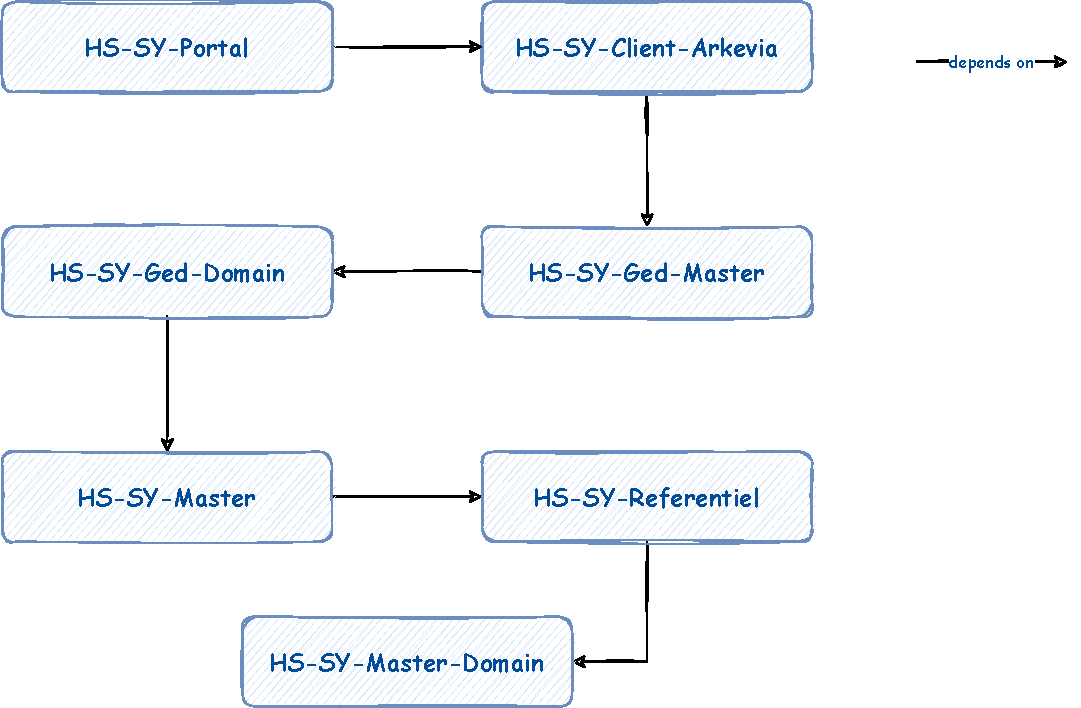
\includegraphics[width=0.6\linewidth]{images/sec4/dep.pdf}
        \caption{Architecture modulaire d'Arkevia}
        \label{fig:modules_arkevia}
    \end{center}
\end{figure}
\subsubsubsection{Renoncer à recourir à la brique de contrôle}
La brique de contrôle (Semantic Model And Business Control) est un service web tiers utilisé pour charger des métadonnées qui servent principalement d'en-tête pour le tableau de description des documents.\\
Suite à un audit mené sur l'application Arkevia afin d'identifier et de déboguer les réponses des appels provenant de cette brique, un total de douze appels a été relevé dans le code de l'application. En effet, cette brique de contrôle soulève des problèmes de performance, notamment un problème de temps d'arrêt très élevé. Afin d'éviter ce goulot d'étranglement, il a été convenu d'éliminer cette dépendance et de la remplacer par un simple appel à la base de données compte tenu que les réponses provenant de cette brique ne sont rien d'autre que des données et des configurations statiques.
\subsubsubsection{Retrait des dépendances inutilisables}
C'est un scénario typique, lorsque l'application est en cours de développement, et que plusieurs membres de l'équipe travaillent dessus, on risque de se trouver face à une série de dépendances inutiles dans les fichiers pom.xml du projet.\\
Il est alors ardu de déterminer manuellement quels sont les jars que l'application ne requiert pas. Pour résoudre ce problème, nous pouvons nous servir du plugin maven-dependency, en particulier l'objectif \lstinline|dependency:analyze|, qui permet d'analyser les dépendances du projet et de déterminer celles qui sont : utilisées et déclarées ; utilisées et non déclarées ; utilisées et déclarées.
\subsubsection{Optimisation du mécanisme d'envoi des notifications}
Le mécanisme de notification est responsable de prévenir un utilisateur par email lorsqu'il y a un nouveau dépôt de document (par exemple un bulletin de salaire) sur son coffre-fort par l'entreprise à laquelle il est abonné.\\

Prérequis nécessaire à la compréhension de sujet :
\begin{itemize}
    \item \textbf{Document} :  bulletins de paie, ou tout autre document RH au format dématérialisé.
    \item \textbf{Lot de documents} :  un nombre limité (batch) de documents (ajustables).
    \item \textbf{Notification} : Un mail générique transmis à un utilisateur pour le notifier du dépôt d'un document.
    \item \textbf{Scan} : une requête lancée à l'API SignArchive afin de vérifier s'il y a des dépôts de documents.
    \item \textbf{Cron} : une tâche planifiée qui déclenche l'exécution du Scan toutes les deux heures (configurable).
\end{itemize}
\subsubsubsection*{Récupération de données}
Le processus de notification est déclenché toutes les deux heures grâce à l'annotation \textbf{@Scheduled} fournie par Spring.\\
Tout d'abord, nous récupérons la date du dernier scan effectué, et nous enregistrons le nouveau scan avec la date du jour dans la table \lstinline|GED_BATCH_SCAN_UPLOAD_DOC|. Le date du dernier scan est utilisé par la suite, pour récupérer tous les documents déposés à partir de cette date jusqu'à le moment de lancement du nouveau scan.
\newpage
\begin{longtblr}[caption={Exemple de déroulement du Cron}]{
    hlines = {0.5pt,chambray},
    vlines = {0.5pt,chambray},
    colsep=4pt,
    rowsep=4pt,
    colspec={Q[l]Q[l]X[l]},
    rowspec={Q[m] Q[m] Q[m] Q[m] Q[m]},
}
\textbf{Scan} & 
\textbf{Date}& 
\textbf{Documents à traiter}\\
1 & 03/02/2021 10:00:00 & Tout dépôt entre 03/02/2021 08:00:00 et 03/02/2021 10:00:00\\
2 & 03/02/2021 12:00:00	& Tout dépôt entre 03/02/2021 10:00:00 et 03/02/2021 12:00:00\\
3 & 03/02/2021 14:00:00	& Tout dépôt entre 03/02/2021 12:00:00 et 03/02/2021 14:00:00\\
...	& ... & ...
\end{longtblr}
La récupération des données est faite à l'aide de la méthode \lstinline|getLastPushedFiles(Date lastDateScan, int indexStart, int count, Client client)|. Cette méthode permet de récupérer un nombre défini de dépôts émis dans un intervalle de temps donné.

\begin{longtblr}[caption={Description des paramètres de la fonction \lstinline|getLastPushedFiles|}]{
    hlines = {0.5pt,chambray},
    vlines = {0.5pt,chambray},
    colsep=4pt,
    rowsep=4pt,
    colspec={Q[l]X[l]},
    rowspec={Q[m] Q[m] Q[m] Q[m] Q[m]},
}
\textbf{Paramètre} & 
\textbf{Description}\\
lastDateScan & c'est la date du dernier scan enregistré dans la table \lstinline|GED_BATCH_SCAN_UPLOAD_DOC|\\
indexStart & permet de spécifier l'indice du premier élément du lot\\
count & permet de spécifier la taille du lot\\
client & le nom du client (toujours "arkevia")\\
\end{longtblr}
Le fonctionnement dernière consiste à:
\begin{itemize}
    \item Construire les critères de recherche.
    \item Appeler la méthode \lstinline|findDocumentByCriteria| du service \lstinline|GedService|.
    \item Interroger l'API SignArchive au moyen d'une requête Solr.
\end{itemize}
\subsubsubsection*{Traitement de données}
Une boucle explore chaque document de la façon suivante :
\newpage
\begin{lstlisting}[numbers=none]
do {Traitement}
while (totalPageNumber > pageIndex)
// totalPageNumber : nombre total des documents divisé par 20
// pageIndex : nombre des lots traités
\end{lstlisting}
\textbf{Traitement :}
\begin{itemize}
    \item Vérifier la validité du matricule et de son propriétaire. 
    \item Rechercher l'utilisateur lié à ce matricule et récupérer son adresse mail.
    \item Vérifier s'il y a déjà une notification envoyé vers cet utilisateur pour ce document - les notifications sont persistés dans la table \lstinline|DocumentUploadNotification|.
    \item Préparer un nouveau objet de notification avec les informations (date, id du document, id de l'utilisateur, etc.).
    \item Persister cet objet dans la base de données et l'ajouter dans une file d'attente (sans envoyer la notification immédiatement).\\
\end{itemize}
Le schéma suivant (figure \ref{fig:seq}) illustre l'approche employée pour traiter ces lots de données :
\begin{figure}[H]
    \begin{center}
        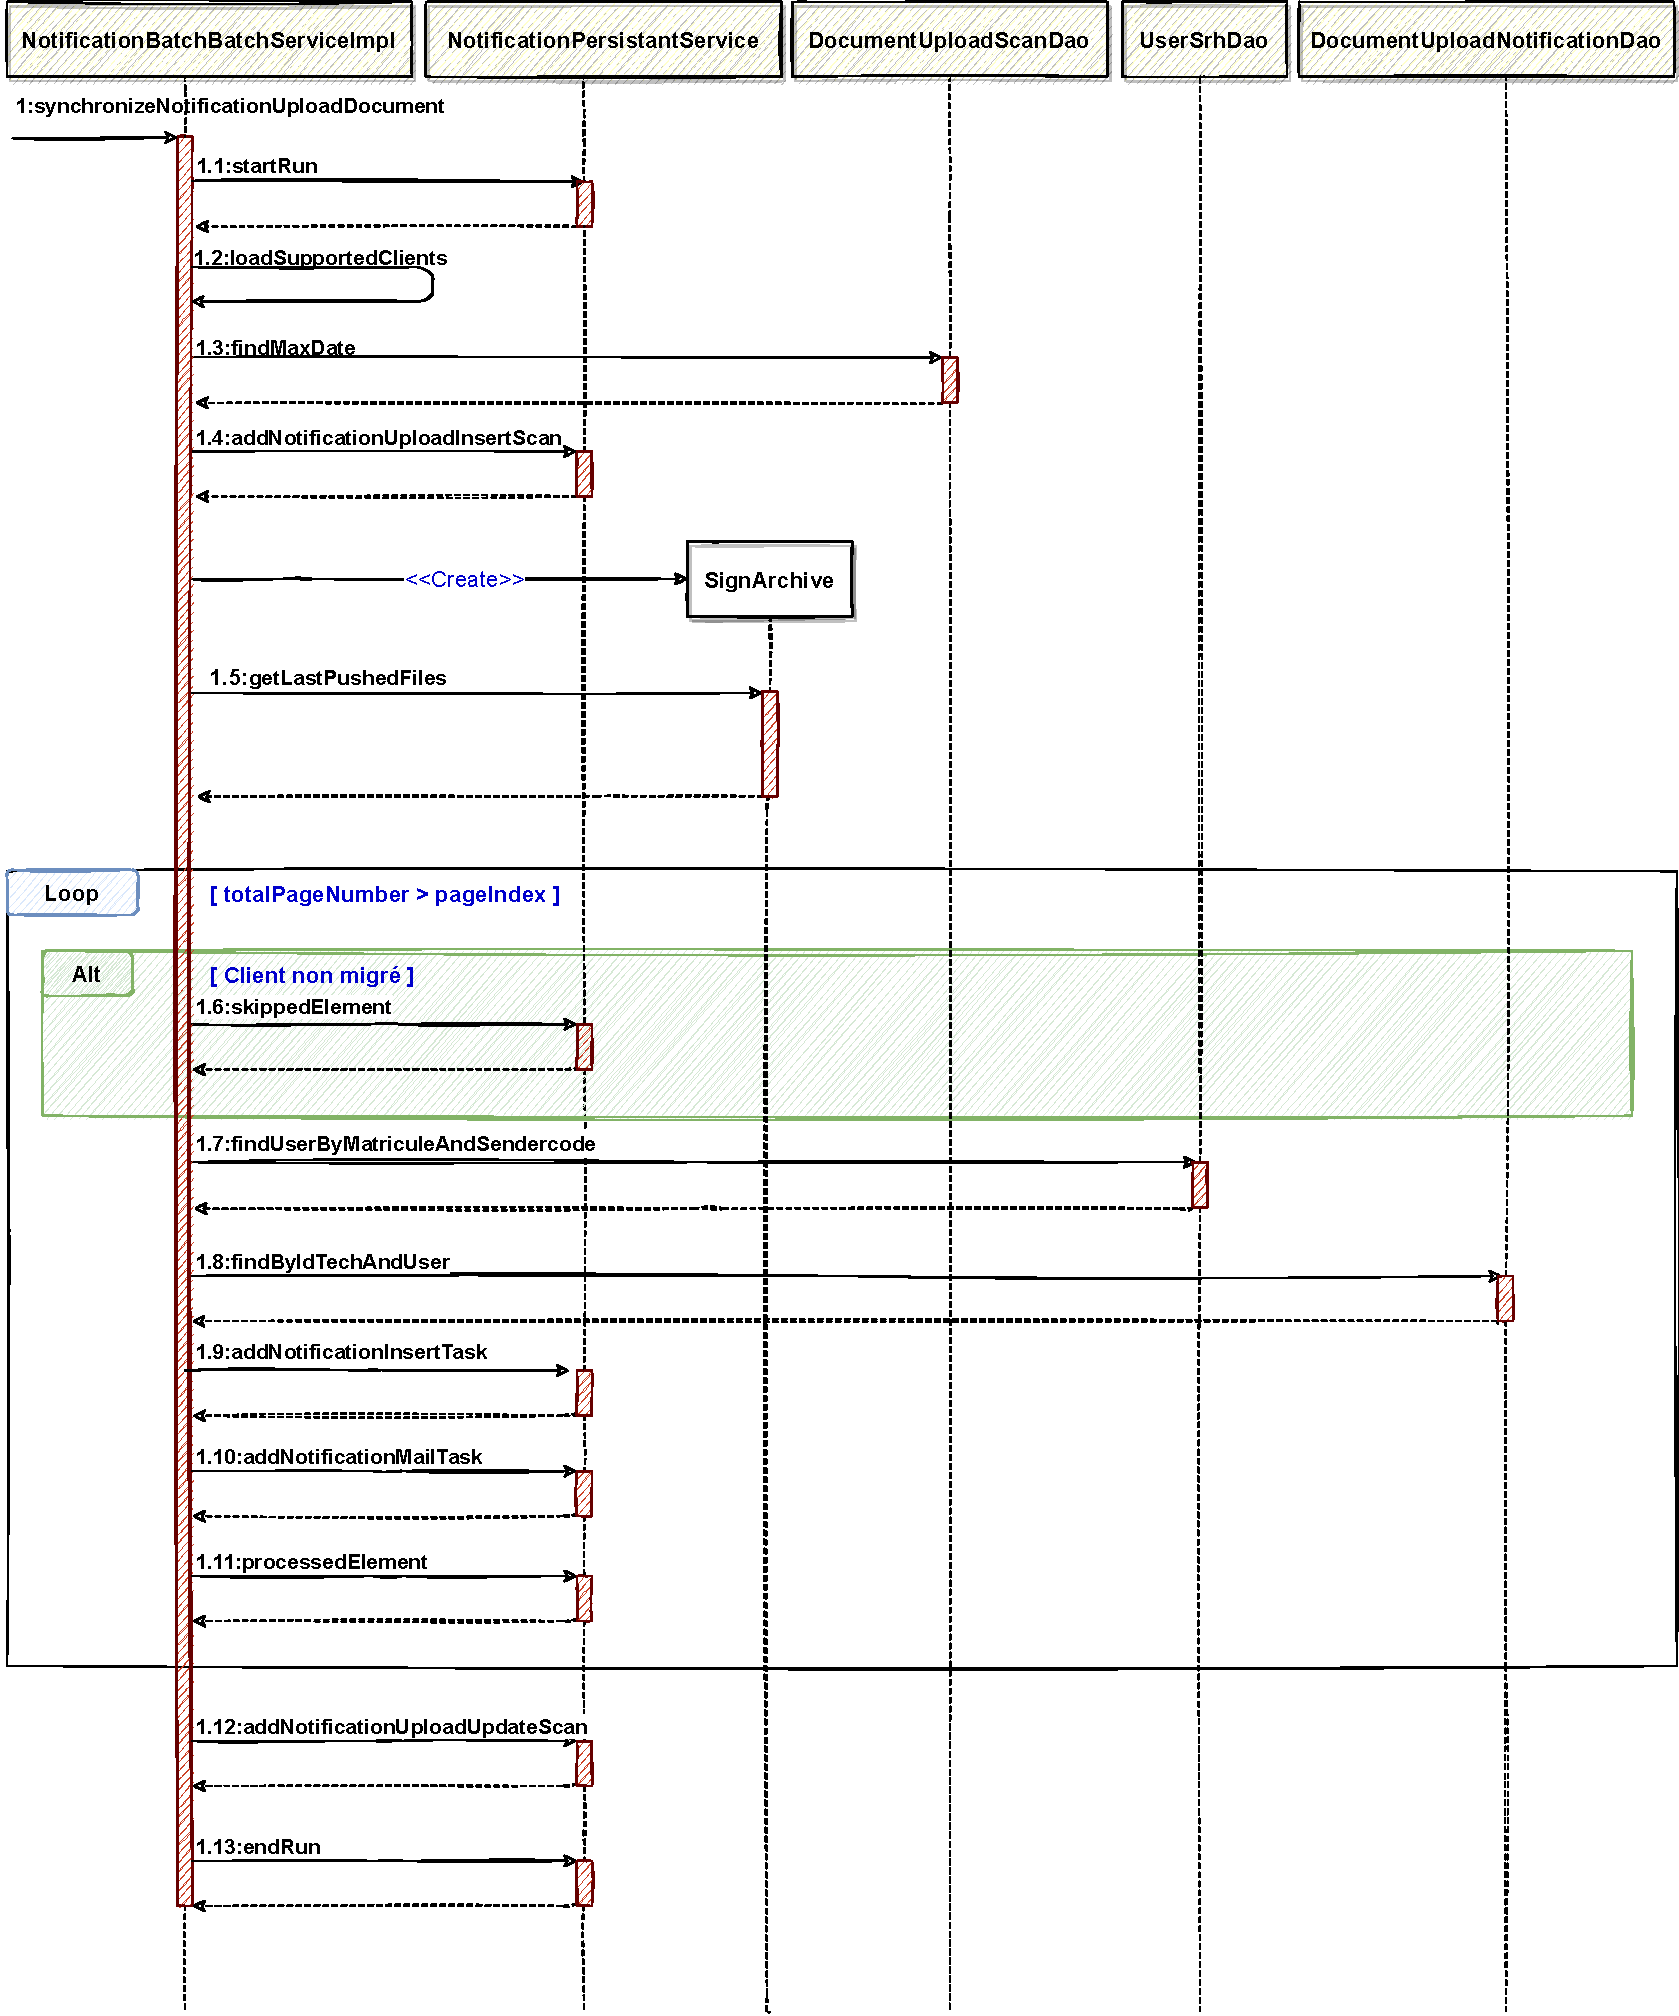
\includegraphics[width=\linewidth]{images/sec4/seq.pdf}
        \caption{Diagramme de séquence modélisant le processus d'envoi de notifications}
        \label{fig:seq}
    \end{center}
\end{figure}
\subsubsubsection*{Problématique et limites}
\begin{itemize}
    \item Mauvaise gestion des indices de recherche pour la méthode \lstinline|getLastPushedFiles|, ce qui conduit à boucler sur les documents déjà traités, et par conséquent à dépenser plus de ressources et de temps.\\

    \item L'appel Solr est couteuse en terme de temps, l'ancien mécanisme sollicite Solr pour chaque 20 documents (c'est-à-dire, si on a 1000 documents $\Longrightarrow$ on doit le solliciter 50 fois). 
    
    \item La réponse de Solr ne parvient pas à distinguer les clients migrés des clients non migrés, et l'ancien mécanisme prend en compte tous les documents, y compris ceux des clients qui n'ont pas encore migré. Le traitement de documents non pertinents exige un temps considérable.
\end{itemize}
\subsubsubsection*{La nouvelle approche}
Le nouveau système prévu devrait reposer sur des paradigmes de multithreading permettant le traitement parallèle de plusieurs lots de données. Ce mécanisme devrait aussi engendrer des changements majeurs dans le processus d'extraction et d'exploitation des données, notamment en ignorant les documents associés aux clients non migrés et en intégrant un service de monitoring qui permettra d'envoyer régulièrement aux superviseurs des courriels comprenant des statistiques sur chaque fichier traité.\\


\addcontentsline{toc}{subsection}{Conclusion}
\subsection*{Conclusion}
En clair, comme nous venons de le voir, ce chapitre a été largement consacré à une conception détaillée de l'application à travers les diagrammes UML et les descriptions textuelles des cas d'utilisation qui nous ont permis notamment de bien appréhender le fonctionnement de l'application, mais surtout de faciliter le processus d'identification des exigences liées au sujet lesquelles ont fait l'objet de la deuxième partie du chapitre. À présent, nous sommes en mesure d'entamer la partie réalisation.
%%%%%%%%%%%%%%%%%%

% %%%%%%%%%%%%%%%%%%%%%%%%%%%%%%%%%%%%%%%%%%%%%%%%%%%
%% Environnement et outils
%%%%%%%%%%%%%%%%%%%%%%%%%%%%%%%%%%%%%%%%%%%%%%%%%%%
\section{Environnements et outils}
\addcontentsline{toc}{subsection}{Introduction}
\subsection*{Introduction}

Après avoir présenté les différentes étapes de conception et la méthodologie suivie, nous présenterons dans ce chapitre les outils de développement et les différents composants logiciels et matériels, pour lesquels constituent la mise en œuvre effective des différentes tâches du sujet.

\subsection{Composants logiciels}
\subsubsection{Front-end}
\begin{longtblr}[caption={Technologies utilisées au niveau du front-end}]{
    hlines = {0.25pt,cyan6},
    vlines = {0.25pt,cyan6},
    row{odd} = {bg=cyan9!10!white},
    colsep=4pt,
    rowsep=4pt,
	colspec={cX},
    rowspec={Q[m] Q[m] Q[m] Q[m] Q[m] Q[m]},
}
{

\includegraphics[height=8mm]{images/sec5/bootstrap.pdf}
\\\textbf{Bootstrap}
}
& 
Bootstrap est un framework front-end extrêmement robuste permettant de développer des applications et des sites Web de manière plus rapide et plus conviviale. Il comprend des modèles de conception basés sur HTML et CSS pour les composants d'interface utilisateur courants tels que les formulaires, les boutons, les tableaux, les navigations, les alertes, les onglets et bien d'autres, ainsi que les extensions JavaScript optionnelles.
Bootstrap offre également la possibilité de créer des mises en page réactives (responsive design) avec un effort minimal.\\

{

\includegraphics[height=6mm]{images/sec5/elementui.pdf}\\\textbf{Element UI}
}
& 
Element est une bibliothèque de composants d'interface utilisateur basée sur Vue 2.0 et qui jouit du soutien d'une large communauté. Elle n'est pas seulement destinée aux développeurs front-end, mais fournit également un kit d'interface utilisateur complet avec lequel les concepteurs et les chefs de produit peuvent travailler. Elle est spécifiquement conçue pour la création d'interfaces utilisateur de bureau, mais prend en charge certaines fonctionnalités réactives telles que le masquage des éléments en fonction de la taille de la fenêtre et la création de grilles.
\\

{
\includegraphics[height=5.5mm]{images/sec5/jquery.pdf}
 \\\textbf{jQuery}
}
&  
\begin{minipage}{\linewidth}
jQuery est une bibliothèque JavaScript libre créée pour faciliter l'écriture de scripts côté client dans le code HTML des pages web. Elle propose comme principales fonctionnalités :
\raggedright
\begin{itemize}[leftmargin=*]
\item La manipulation du Document Object Model (DOM).
\item La gestion des événements (mouvements de souris, clics, etc.) et de l'AJAX.
\item La création d'effets d'animation.
\item La manipulation des feuilles de style en cascade.
\end{itemize}
\end{minipage}
\\
{
\includegraphics[height=5.5mm]{images/sec5/jqueryui.pdf}
 \\\textbf{jQuery UI}
 }
 & 
 \begin{minipage}{\linewidth}
	jQuery UI est une bibliothèque JavaScript basée sur jQuery, fournissant une collection d'éléments utiles au développement d'interfaces utilisateur. Ces éléments comprennent :
\begin{itemize}[leftmargin=*]
	\item Des interactions comme le "drag \& drop" (glisser-déposer)
	\item Des "widgets" (composants d'interface graphique) telles que les barres de progression, les infobulles, etc.
	\item Des effets pour modifier dynamiquement l'apparence des éléments de l'interface (par exemple, changer la couleur, faire apparaître/disparaître un élément, etc.)
	\item Des thèmes avec des propriétés CSS pour la mise en page des éléments interactifs.
\end{itemize}
\end{minipage}
 \\
 {
\includegraphics[height=8mm]{images/sec5/sass.pdf}
 \\\textbf{Sass}
 }
 & Sass (Syntactically Awesome Style Sheets) est une extension de CSS intégrant des fonctionnalités telles que les règles imbriquées, les variables, les mixins et les extensions de classe. Cela permet aux développeurs d'écrire des CSS structurés, lisibles et réutilisables. Sass est compilé en CSS standard. Il s'agit principalement d'un langage de préprocesseur CSS qui accepte à la fois le CSS et sa syntaxe personnalisée d'écriture de codes de conception visuelle.\\
{
\includegraphics[width=8mm]{images/vuejs.png} \\\textbf{VueJs}
} & Vue (prononcé /vju:/, comme le terme anglais view) est un framework évolutif pour construire des interfaces utilisateur. À la différence des autres frameworks monolithiques, Vue a été conçu et pensé pour pouvoir être adopté de manière incrémentale. Le cœur de la bibliothèque se concentre uniquement sur la partie front-end. D’un autre côté, Vue est tout à fait capable de faire tourner des applications web mono-pages quand il est couplé avec des outils modernes et des bibliothèques complémentaires.\\
\end{longtblr}

\subsubsection{Back-end}
\begin{longtblr}[caption={Technologies utilisées pour les solutions back-end}]{
    hlines = {0.25pt,azure6},
    vlines = {0.25pt,azure6},
    row{odd} = {bg=azure9!10!white},
    colsep=4pt,
    rowsep=4pt,
	colspec={cX},
    rowspec={Q[m] Q[m] Q[m] Q[m] Q[m] Q[m]},
}
{
\includegraphics[height=4.5mm]{images/sec5/hibernate.pdf}
 \\\textbf{Hibernate}
 }
 & Hibernate est une bibliothèque de mappage objet-relationnel (ORM) pour le langage Java permettant aux développeurs d'utiliser des modèles de domaine de style POJO dans leurs applications d'une manière qui va bien au-delà du mappage objet/relationnel.\\
 {
\includegraphics[width=7mm]{images/sec5/java.pdf}
 \\\textbf{Java}
 }
 & JAVA est un langage de programmation de haut niveau, orienté objet, fonctionnel, indépendant de la plate-forme et un environnement d'exécution.
 Le langage Java tire une grande partie de sa syntaxe du C et du C++, mais son modèle objet est plus simple que celui de ce dernier et il a moins de facilités de bas niveau. Les applications Java sont généralement compilées en bytecode (appelés fichiers de classe) qui peuvent être exécutés par une JVM (Java Virtual Machine), indépendamment de l'architecture informatique. La JVM compile souvent le code en code machine natif pour optimiser les performances.\\
{

\includegraphics[height=6.5mm]{images/sec5/log4j.png}
\\\textbf{Log4j}
}
& Log4j est un outil de journalisation permettant de personnaliser les logs propres à chaque programme. Il peut être utile pour le débogage ou le traçage de l'exécution d'un programme.\\
{

\includegraphics[height=5.5mm]{images/sec5/spring.pdf}
\\\textbf{Spring}
}
& 
Spring est un framework open source fournissant une boite à outils très riche permettant de structurer, d'améliorer et de simplifier l'écriture d'application Java. Spring est également livré avec une variété de modules dédiés à l'exécution de différentes tâches. Certains d'entre eux sont Spring Test, Spring Security, Spring Web, Spring JDBC, Spring AOP, Spring MVC et Spring ORM.\\

{

\includegraphics[height=5.5mm]{images/sec5/spring.pdf}\\\textbf{Spring Batch}
}
& 
Spring Batch est un framework open source basé sur Spring pour permettre le développement d'applications batch qui sont essentielles au fonctionnement quotidien des systèmes d'entreprise. En général, les applications batch font référence à des systèmes automatisés conçus pour traiter des données de masse.
Spring Batch automatise cette itération de base des lots, en offrant la possibilité de traiter des transactions similaires comme un ensemble, souvent dans un environnement isolé, sans aucune interaction avec l'utilisateur.
\\

 {
\includegraphics[height=5.5mm]{images/sec5/spring.pdf}
 \\\textbf{Spring Boot}
 }
&  
\begin{minipage}{\linewidth}
Spring Boot permet de créer facilement une application alimentée par Spring avec un minimum d'effort. Une application créée avec Spring Boot peut être :
\raggedright
\begin{itemize}[leftmargin=*]
\item Créée sans requérir aucune configuration xml.
\item Créé sans aucune exigence de serveur d'application puisque Spring Boot fournit un serveur d'application (Tomcat intégré, Jetty ou Undertow).
\item Largement configuré avec quelques valeurs par défaut et des POM de démarrage pour simplifier la configuration Maven du projet.
\item Fournit des solutions prêtes pour la production telles que les métriques, l'intégrité de performance et la configuration externalisée.
\end{itemize}
\end{minipage}
\end{longtblr}
\subsubsection{Système de gestion de base de données}
Arkevia est conçu pour fonctionner sur une instance Oracle 10g  (ou plus).\\
Le SGBDR \textbf{Oracle} est utilisé par toutes les applications de la solution ARKEVIA. Il dispose aujourd'hui de l'une des meilleures prestations en termes de performance, de scalabilité et d'administration.
\subsubsection{Stockage et sécurité des données}
Le coffre-fort électronique constitue un espace de stockage sécurisé pour les documents qui y sont déposés (EDI, EDI signé, PDF signé).\\
Il permet de garantir :
\begin{itemize}
    \item L'intégrité des documents, au moyen d’une fonction de signature électronique.
    \item La confidentialité des documents, au moyen d’une fonction de chiffrement de données.
    \item La traçabilité des actions effectuées (dépôts, restitutions, demandes de copies, etc.).
    \item Les documents ont ainsi une valeur probante(juridiquement opposable).\\
\end{itemize}
\begin{itemize}[leftmargin=*]
    \item[\textcolor{green5!30!white}{\faCheckCircleO}] Le dépôt ou l'extraction de fichiers ne peut se faire qu'à partir de l'application ARKEVIA, via les Web Services avec authentification SSL Client/Serveur.
    \item[\textcolor{green5!30!white}{\faCheckCircleO}] Les fichiers sont horodatés, signés, chiffrés et stockés dans un espace sécurisé du datacenter de Cegedim.\newpage
    \item[\textcolor{green5!30!white}{\faCheckCircleO}] Le contenu est chiffré avec l'algorithme AES 128 GCM, la clé appartient à Cegedim. Le chiffrement des flux est sécurisé en HTTPS / TLS 1.2 (AES 256) avec un certificat SHA-256 appartenant à Cegedim.
    \item[\textcolor{green5!30!white}{\faCheckCircleO}] Les mots de passe des utilisateurs sont protégés par « hashage » via l'algorithme SHA-256.
\end{itemize}
\subsection{Environnement de développement}
\subsubsection{Environment matériel}
Les tâches assignées ont été élaborées sur un ordinateur de bureau conçu pour réaliser les différentes activités liées aux thèmes du stage, soit directement, soit par le biais du protocole RDP. L'ordinateur fourni a les spécifications matérielles et logicielles suivantes :
\begin{itemize}
    \item \textbf{Fabricant} : Dell Inc.
    \item \textbf{Modèle du système} : OptiPlex 7040
    \item \textbf{Processeur} : [01] : Intel64 Family 6 Model 94 Stepping 3 GenuineIntel ~3312 MHz
    \item \textbf{Mémoire physique totale} :  16 309 Mo
    \item \textbf{Système d’exploitation} : Microsoft Windows 10 Professionnel pour les Stations de travail.
\end{itemize}

\subsubsection{Environnement logiciel et outils}
\begin{longtblr}[caption={Environnements et outils de développement et de collaboration}]{
    hlines = {0.25pt,red7},
    vlines = {0.25pt,red7},
    row{odd} = {bg=red9!10!white},
    colsep=4pt,
    rowsep=4pt,
	colspec={cX},
    rowspec={Q[m] Q[m] Q[m] Q[m] Q[m] Q[m] Q[m] Q[m] Q[m] Q[m] Q[m] Q[m] Q[m] Q[m] Q[m] Q[m] Q[m] Q[m]},
}
{

\includegraphics[height=8mm]{images/sec5/confluence.pdf}
\\\textbf{Confluence}
}
& 
Atlassian Confluence est un système de collaboration et de wiki pour les entreprises.
Atlassian Confluence est utilisé pour la collaboration, la gestion de la base de connaissances, la rédaction technique et en tant qu'intranet social ou gestionnaire de documents.\\

{

\includegraphics[height=8mm]{images/sec5/gitlab.pdf}\\\textbf{GitLab}
}
& 
GitLab est une plateforme DevOps complète proposée sous la forme d'une application unique. Elle révolutionne le développement, la sécurité, l'exploitation et la collaboration entre les équipes. 
\\

{
\includegraphics[height=7.5mm]{images/sec5/intellijidea.pdf}
 \\\textbf{Intellij IDEA}\\(Ultimate Edition)
}
&  
Intellij IDEA est un IDE complet développé par JetBrains (anciennement « IntelliJ ») axé sur la productivité avec des systèmes d’autocomplétion intelligente, d’analyse de code en temps réel, de refactoring avancé ; l’intégration d’outils de tests et de debugging ; et une pléthore de raccourcis clavier permettant de réaliser rapidement presque toutes les tâches.
\\
{
\includegraphics[height=8mm]{images/sec5/jira.pdf}
 \\\textbf{Jira}
 }
 & 
 \begin{minipage}{\linewidth}
	jQuery UI est une bibliothèque JavaScript basée sur jQuery, fournissant une collection d'éléments utiles au développement d'interfaces utilisateur. Ces éléments comprennent :
\begin{itemize}[leftmargin=*]
	\item Des interactions comme le "drag \& drop" (glisser-déposer)
	\item Des "widgets" (composants d'interface graphique) telles que les barres de progression, les infobulles, etc.
	\item Des effets pour modifier dynamiquement l'apparence des éléments de l'interface (par exemple, changer la couleur, faire apparaître/disparaître un élément, etc.)
	\item Des thèmes avec des propriétés CSS pour la mise en page des éléments interactifs.
\end{itemize}
\end{minipage}
 \\
 {
\includegraphics[width=8mm]{images/sec5/excel.pdf} \\\textbf{Microsoft Excel}
} & Vue \\
{
\includegraphics[width=8mm]{images/sec5/outlook.pdf} \\\textbf{Microsoft Outlook}
} & Vue \\
 {
\includegraphics[width=8mm]{images/sec5/powerpoint.pdf}
 \\\textbf{Microsoft}\\\textbf{PowerPoint}
 }
 & Sass.\\
 {
\includegraphics[width=8mm]{images/sec5/word.pdf} \\\textbf{Microsoft Word}
 } & Vue \\
 {
\includegraphics[height=8mm]{images/sec5/oraclesqldeveloper.pdf} \\\textbf{Oracle SQL}\\\textbf{Developer}
} & Vue \\
{
\includegraphics[height=7mm]{images/sec5/postman.pdf} \\\textbf{Postman}
} & Postman est un environnement de développement d'API complet permettant de concevoir, de mocker, de tester, de surveiller et de publier des API à partir de l'interface utilisateur Postman.\\
{
\includegraphics[height=7mm]{images/sec5/sonarcube.pdf} \\\textbf{SonarQube}
} & Vue \\
{
\includegraphics[width=7mm]{images/sec5/sourcetree.pdf} \\\textbf{Sourcetree}
} & Vue \\
{
\includegraphics[height=8mm]{images/sec5/wildfly.pdf} \\\textbf{WildFly}
} & Vue \\
{\includegraphics[height=4.5mm]{images/sec5/zoom.pdf} \\\textbf{Zoom}
} & Vue \\
\end{longtblr}
\subsection{Outils utilisés pour la réalisation de ce rapport}
Adobe Illustrator
Draw.io
LaTeX
Figma
Vs code
\addcontentsline{toc}{subsection}{Conclusion}
\subsection*{Conclusion}
%%%%%%%%%%%%%%%%%%

% %%%%%%%%%%%%%%%%%%%%%%%%%%%%%%%%%%%%%%%%%%%%%%%%%%%
%% Conclusion
%%%%%%%%%%%%%%%%%%%%%%%%%%%%%%%%%%%%%%%%%%%%%%%%%%%

\phantomsection
\markboth{CONCLUSION GÉNÉRALE}{}
\addcontentsline{toc}{section}{Conclusion générale}
\section*{Conclusion générale}

Dans l'ensemble, je retiens un bilan positif de mon stage de fin d'études : J'ai pu intégrer une équipe de recherche et développement (R\&D) polyvalente travaillant principalement autour des technologies Java et JavaScript. Cela m'a donné une idée concrète des exigences de Cegedim en matière d'ingénierie de développement orienté objet, ainsi que sur les règles et les bonnes pratiques de la gestion de projet agile, allant de la phase de recueil des besoins jusqu'à celle de la livraison du produit final.\\

La formation acquise dans le cadre de mon Master à la Faculté des Sciences de Rabat, notamment le module d'ingénierie du développement logiciel, m'a été très utile dans diverses situations que ce soit sur le plan conceptuel (élaboration des besoins, étude de faisabilité, conception générale, etc.) ou sur le plan technique (codage, complexité du code, bonnes pratiques de développement, etc.) ou encore sur le plan relationnel (travail collaboratif, planification et gestion de projets, etc.).\\

Ce stage a été très enrichissant pour moi, car il m'a permis de découvrir le monde du SIRH, un domaine vaste, nécessitant à la fois un esprit d'analyse sceptique et de solides compétences techniques. De surcroît, cette expérience m'a permis de participer concrètement à ses enjeux à travers des missions de développement et de refonte.\\

Ce rapport présente les différentes tâches réalisées durant ma période de stage, à savoir la migration du socle technique et le refactoring du code ainsi que la refonte du système délégué d'envoi des notifications. L'élaboration de ce rapport a été entamé par une présentation de l'organisme d'accueil. Par la suite, une étude de l'existant a été réalisée afin d'identifier les problèmes et d'exposer les solutions et les axes d'amélioration. Après cela, une étude conceptuelle détaillée des différentes fonctionnalités a été mise en place de même que la définition des besoins et les contraintes du projet. Enfin, ce rapport se termine par l'exposition des outils et de l'environnement de travail et aussi par une démonstration sur une solution réalisée pour remédier aux inconvénients de l'ancien système d'envoi de notifications.\\

Au terme de ce mémoire, je pense que ce stage en entreprise m’a offert une bonne préparation pour mon insertion professionnelle, car il fut une expérience enrichissante et complète qui conforte le désir d’exercer un futur métier dans le domaine de l’informatique. D'autre part, l'environnement professionnel dans lequel s'est déroulé ce stage m'a fait découvrir de nouvelles connaissances et compétences et a renforcé mon esprit d'équipe et mon professionnalisme. Cette expérience a aiguisé mes capacités d'analyse et de synthèse et a surtout renforcé mon esprit critique, ma motivation et mon ambition.\\
Enfin, je tiens à exprimer ma satisfaction d’avoir pu travailler dans de bonnes conditions matérielles et un environnement agréable.
\phantomsection
\begin{appendices}
\titleformat{\section}
{\color{chambray}\normalfont\Large\bfseries}{}{1em}{}
\section{ANNEXES}
\markboth{ANNEXES}{}
\subsection{Présentation des principales interfaces d'Arkevia}
\null\vfill
\begin{figure}[H]
    \begin{center}
        \includegraphics[width=\linewidth]{images/annexes/scr1.png}
        \caption{Page d'authentification Arkevia}
        \label{fig:arkevia1}
    \end{center}
\end{figure}
\vfill\null
\clearpage
\null\vfill
\begin{figure}[H]
    \begin{center}
        \includegraphics[width=\linewidth]{images/annexes/scr2.png}
        \caption{Page de gestion des documents}
        \label{fig:batch}
    \end{center}
\end{figure}
\vfill\null
\begin{figure}[H]
    \begin{center}
        \includegraphics[width=\linewidth]{images/annexes/scr3.png}
        \caption{Page de gestion de compte Arkevia}
        \label{fig:batch}
    \end{center}
\end{figure}
\subsection{Audit de code : checklist élaborée par Cegedim SRH}
\label{sec:checklist}
\begin{longtblr}[caption={Extrait des règles et pratiques de développement logiciel instaurées par Cegedim SRH}, label={tab:dev}]{
    hlines = {0.25pt,azure6},
    vlines = {0.25pt,azure6},
    colsep=4pt,
    rowsep=4pt,
	colspec={QX},
}
\textbf{Réf.} & \textbf{Description de la règle}\\
RG\_DEV\_GN\_001 & Single responsibility principle :
Une fonction doit être responsable d'une et d'une seule tâche. Lorsqu'une fonction fait plus d'une tâche, elle est plus difficile à composer, à tester et à comprendre.\\
RG\_DEV\_GN\_002 & Don't repeat yourself :
Souvent, nous avons du code en double parce que nous avons deux ou plusieurs choses légèrement différentes, qui partagent beaucoup en commun, mais leurs différences nous obligent à avoir deux ou plusieurs fonctions distinctes qui font en grande partie les mêmes choses. Supprimer le code en double signifie créer une abstraction qui peut gérer cet ensemble de choses différentes avec une seule fonction / module / classe.
Factoriser le code en double.\\
RG\_DEV\_GN\_003 & Open/Closed principle :
Les nouvelles fonctionnalités ne doivent pas modifier le code existant.\\
RG\_DEV\_GN\_004 & Test unitaire :
Chaque fonction doit être testée avec au minimum un cas passant et un cas non passant.\\
RG\_DEV\_GN\_005 & Respect des warnings eslint sonarLint :
Veiller au maximum à ce qu’il n’y a pas de warnings eslint et/ou sonarlint dans la classes/ou parties de classes impactées dans le cadre d’une évolution, l’objectif est d’atteindre 0 Warnings dans le possible.\\			
RG\_DEV\_GN\_006 & Correction des NullPointerException :
Éviter de contourner le problème de nullité en ajoutant des tests, et aller plus en profondeur dans le diagnostic pour détecter l’origine du problème et le résoudre d’une manière radicale.\\
RG\_DEV\_GN\_007 & Arguments de fonctions :
Limiter le nombre de paramètres d'une fonction est extrêmement important, un ou deux arguments est le cas idéal, et trois devraient être évités si possible. Rien de plus que cela devrait être utilisé. Utiliser des objets si nous avons besoin de beaucoup d'arguments.\\			
RG\_DEV\_GN\_008 & Cas des dépassements de capacité :
Éviter de contourner le problème en tronquant des valeurs, et aller plus en profondeur dans le diagnostic pour détecter l’origine du problème et le résoudre d’une manière radicale.
% RG_DEV_GN_008	O		Cas des « prepared statement »  :
% Utiliser systématiquement les « prepared statment » à chaque fois quand c’est possible, et respecter la charte de nommage sur la partie PS.			
% RG_DEV_GN_009	O		Code en dur dans les programmes 
% Eviter le code en dur dans les programmes pour une meilleure évolutivité			
% RG_DEV_GN_010	O		Table en mémoire :
% Eviter de charger les tables en mémoire pour de meilleures performances.
% Exemple :
% Ne pas charger toutes les données d'une table de référence dans une liste d'objets.			
% RG_DEV_GN_011	O		Valeurs par défaut :
% Privilégier l'utilisation des valeurs par défaut dans les fonctions.			
% RG_DEV_GN_012	O		Eviter l'utilisation des flags comme des paramètres de fonction
% Diviser les fonctions si elles suivent des chemins de code différents en fonction d'un booléen.			
% RG_DEV_GN_013	O		Eviter les conditions négatives			
% RG_DEV_GN_014	O		Eviter les conditions imbriquées (au dessous 2 niveaux )			
% RG_DEV_GN_015	O		Supprimer le code mort			
% RG_DEV_GN_015	O		Privilégier l'utilisation des getters et des setters			
% RG_DEV_GN_016	O		Nomenclature :
% Utiliser des noms de variables, de fonctions et de classes significatifs et pronoçables:			
% RG_DEV_GN_017	O		• Un identifiant représentant une collection d’objets doit être un nom au pluriel (utiliser de préférence le nom de l’objet) précédé de "list".
% Exemple :
% private String[] listCountries = null;
% private Personne[] listPersonnes = null;			
% RG_DEV_GN_018	O		• Le terme compute doit être employé dans les méthodes où quelque chose est calculé. Il donne au lecteur l'indice immédiat que c'est potentiellement une opération longue.			
% RG_DEV_GN_019	O		• Le terme find doit être employé dans les méthodes où quelque chose est recherché. Elle donne au lecteur l'indice immédiat que la méthode est une simple recherche avec un minimum de calculs.
% Exemple :
% matrice.findMinElement()			
% RG_DEV_GN_020	O		• Le terme initialize doit être employé là où un objet ou un concept est construit. L'abréviation d'init peut également être employée.
% Exemple :
% printer.initializeFontSet();
% printer.initFontSet();			
% RG_DEV_GN_021	O		• Des noms de concept complémentaire doivent être employés pour des comportements complémentaires.
%  get/set, add/remove, start/stop, insert/delete, increment/decrement, old/new, begin/end, first/last, up/down, min/max, next/previous, old/new, open/close, show/hide, create(ou New)/destroy.			
% RG_DEV_GN_022	O		• Les méthodes de mise à jour, suppression et insertion de données sont préfixées respectivement par update, delete et insert.			
% RG_DEV_GN_023	O		• Les constantes d'un même concept doivent être réunies et préfixées par un nom commun de type. Ceci indique que les constantes appartiennent au même ensemble, et permet d'identifier le concept représenté.
% • Attention néanmoins à éviter les tautologies (par exemple : Color.COLOR_RED).
% Exemple :
% static final int COLOR_RED   = 1;
% static final int COLOR_GREEN = 2;
% static final int COLOR_BLUE  = 3;			
% RG_DEV_GN_024	O		Commit tout azimut :
% Eviter de mettre des Commit/Rollback intermédiaires dans les étapes des étapes du Batch, un commit ou Rollback doivent être positionnés à la fin des étapes. 			
% RG_DEV_GN_025	O		Commentaire :
% Mettre un nombre de commentaires considérable pour décrire ce que font les modifications ajoutées, avec un contenu explicite, clair et compréhensible sur ce que fait réellement le code.
% Utiliser au max les formats conventionnés (JSDOC, JavaDoc, ,,,) pour les commentaires			
% Charte Java						
% RG_DEV_JAVA_001	O		Nom Package :
% • Le préfixe d'un nom de package doit correspondre au niveau supérieur d'un nom de domaine : com
% Exemple : 
% package com.ro.framework.batch;			
% RG_DEV_JAVA_002	O		Décomposition domaine : 
% • Un domaine est décomposé en plusieurs procédures.
% Exemple : 
% package com.ro.domaine.procedure;			
% RG_DEV_JAVA_003	O		Nom Classe :
% • Le nom d'une classe ne doit pas comporter d'information concernant son mode d'implémentation, celui-ci pouvant évoluer pendant le cycle de vie de l'application.			
% RG_DEV_JAVA_004	O		• Si le nom d'une classe comporte des informations concernant son type technique (Exception, Trace, Objet métier, etc.) ou le type de concept implémenté (Factory, Facade, etc.), ces informations doivent être suffixées.
% Exemple :
% class IRuntimeNavigationFactory // Interface d’une fabrique/usine
% class NavigationFactoryBuilder  // Fabrique d’usine
% class BeneficiaireSingleton  // Singleton
% class ProcessAccessCfg // Configuration
% class TechnicalException // Exception technique
% class DevisBOModel  // Modèle métier
% class MethodInvokerTools // Utilitaires
% class ProcessAccessManagerTest // Test			
% RG_DEV_JAVA_005	O		• Il est courant de créer une implémentation simpliste de classe ou d'une interface fournissant le comportement par défaut aux méthodes d'interface. Dans ce cas, l'implémentation peut être suffixée par Default.
% Exemple :
% class DefaultManager implements IManager;			
% RG_DEV_JAVA_006	O		• Une normalisation particulière est appliquée aux classes Actions.
% • Mot Clé « Map » suivi d’un mnémonique pour le mapping.
% • Mot Clé « Pop » suivi d’un mnémonique pour le populing.
% Exemple :
% class MapListePersonnes;
% class PopListePersonnes;			
% Charte JavaScript						
% RG_DEV_JS_001	O		Déclaration des variables:
%     * Utiliser "const" par défaut
%     * Utiliser "let" si la variable va être modifier
%     * Ne pas utiliser "var"			
% RG_DEV_JS_002	O		Modifier un objet ou un tableau au sein d'une fonction risque d'avoir des effets secondaires.
% La solution est de cloner le tableau / objet par la fonction, modifier et ensuite renvoyer la clone, ça garantit que les autres fonctions qui utilisent toujours l'ancien tableau / objet ne seraient pas affectées par les modifications.			
% RG_DEV_JS_003	O		Tyepes des variables :
% Etant donné que JavaScript n'est pas langage typé, éviter au maximum la vérification du type:
%     * instanceof
%     * typeof			
% RG_DEV_JS_004	O		Traitements asynchrones :
% Privilégier l'utilisation des "promises" au lieu des "deffered"
% Ne pas ignorer les promesses rejetées			
% Charte VueJS						
% RG_DEV_VUE_001	O		• Tous les noms de composants doivent être en minuscule,
% Exemple : register-component.vue			
% RG_DEV_VUE_002	O		Les noms de composant devraient toujours être des mots multiples (separés par un tiret), à l’exception du composant racine App et des composants préconçus fournis par Vue comme <transition> ou <component>. (pour prévenir les conflits)
% Exemple:
% register-header-component.vue			
% Charte MongoDB						
% RG_DEV_MONGO_001	O		La taille maximale d'un document MongoDB est de 16MB			
% RG_DEV_MONGO_002	O		Nom Collection et Index :
% - Noms en minuscules: évite les problèmes de sensibilité, les noms de collections MongoDB sont sensibles à la casse.
% Pluriel: plus évident pour étiqueter une collection de quelque chose comme pluriel, par exemple “fichiers” plutôt que “fichier”

% - Pas de séparateur de mots: évite les problèmes où des personnes différentes (à tort) séparent les mots (username <-> user_name, first_name <-> firstname). .

% - Notation par points pour les collections plus détaillées: donne des indications sur la manière dont les collections sont liées. Par exemple, vous pouvez être raisonnablement sûr de pouvoir supprimer “users.pagevisits” si vous avez supprimé “users”, à condition que les personnes qui ont conçu le schéma aient fait du bon travail.			
% RG_DEV_MONGO_003	O		Nom Collection et Index :
% - Noms en minuscules: évite les problèmes de sensibilité, les noms de collections MongoDB sont sensibles à la casse.
% Pluriel: plus évident pour étiqueter une collection de quelque chose comme pluriel, par exemple “fichiers” plutôt que “fichier”

% - Pas de séparateur de mots: évite les problèmes où des personnes différentes (à tort) séparent les mots (username <-> user_name, first_name <-> firstname). .

% - Notation par points pour les collections plus détaillées: donne des indications sur la manière dont les collections sont liées. Par exemple, vous pouvez être raisonnablement sûr de pouvoir supprimer “users.pagevisits” si vous avez supprimé “users”, à condition que les personnes qui ont conçu le schéma aient fait du bon travail.			
% RG_DEV_MONGO_004	O		Plutôt que de récupérer l'intégralité du document, de mettre à jour les champs, puis de réenregistrer le document dans la base de données, émettez plutôt une mise à jour sur des champs spécifiques. Cela présente l'avantage de réduire l'utilisation du réseau et la surcharge de base de données.			
% Charte de structure et organisation						
% RG_STRUCT_001	O		Conventions de nommage :
%     * Les noms des composants de la libSmart: cs-xxx-yyy
%     * Les noms des fichiers des composants vue: csXxxYyy
%     * Les noms des composants métiers: camelCase
%     * Les noms des fichiers JS des composants métiers: camelCase
%     * Les noms des variables: camelCase
%     * Les noms des classes CSS: cs-xxx-xxx
%     * Les noms des scripts: wc_xxxYyy
%     * Les noms des libelles: snacke_case
%     * Les noms des méthodes: camelCase			SMART
% RG_STRUCT_002	O		Architecture du projet :
%     * Chaque module doit avoir son propre dossier
%     * Chaque module doit avoir son propre fichier de style
%     * Chaque module doit avoir son propre store
%     * Le composant métier doit être découpé:
%         ** Un fichier JS pour son template
%         ** Un fichier JS pour son script			SMART
% RG_STRUCT_003	O		Chemin d'accès :
% • Les pages sont situés sous " <APP> \sy-portal\HS-SY-Portal\src\main\webapp\portal\client"
% Exemple : <APP> \sy-portal\HS-SY-Portal\src\main\webapp\portal\client\arkevia\home\home-component.vue			ARKEVIA
% RG_STRUCT_004	O		Architecture du projet:
%     * Chaque composant doit appartenir à un seul module 
%     * Chaque composant doit inclure son propre fichier ts (logique du composant) et son fichier de vue (html)
%     * Un composant peut inclure son propre fichier de style 
%     * Un composant peut utiliser d'autres fichiers de style			MOBILE

\end{longtblr}
\subsection{Outils utilisés pour la réalisation de ce rapport}
Ce rapport est basé sur un modèle de rapport pédagogique conçu pour le département d'informatique de l'Université d'Avignon, par son auteur Vincent Labatut.\\
Pour obtenir ce modèle, veuillez visiter le site suivant : \url{https://fr.overleaf.com/latex/templates/modele-de-rapport-avignon-universite/pdbgdpzsgwrt}.\\

Le rapport est compilé à l'aide de \textbf{LuaLaTeX}, une variante de \textbf{LaTeX} utilisant le langage de script \textbf{Lua}. \textbf{LuaTeX} a été choisi comme successeur de \textbf{pdfTeX}. La structure générale et la plupart des commandes sont similaires à celles de LaTeX.\\

Il a également été utile d'utiliser certains supports pour produire les ressources et les illustrations incluses dans le rapport. Le tableau suivant rassemble les différents outils utilisés dans la mise en œuvre de ce rapport.
\begin{longtblr}[caption={Supports utilisés pour la réalisation de ce rapport}]{
    hlines = {0.25pt,cyan6},
    vlines = {0.25pt,cyan6},
    colsep=4pt,
    rowsep=4pt,
	colspec={cX},
    rowspec={Q[m] Q[m] Q[m] Q[m] Q[m] Q[m]},
}

{\includegraphics[height=8mm]{images/annexes/adobecc.pdf}
 \\\textbf{Adobe Illustrator}
}
&  
Adobe Illustrator est un logiciel de création graphique vectorielle. Il fait partie de la gamme Adobe, peut être utilisé indépendamment ou en complément de Photoshop, et offre des outils de dessin vectoriel puissants. Les images vectorielles sont constituées de courbes générées par des formules mathématiques.\\
{\includegraphics[height=8mm]{images/annexes/draw.pdf}
 \\\textbf{Draw.io}
 }
 & 
 Draw.io est une application de création de diagrammes et schémas sous licence Apache disponible sous Windows, macOS, Linux, sous forme d’application web et intégrée à des services cloud tels Nextcloud ou Google Drive.
 \\
 {\includegraphics[height=8mm]{images/annexes/figma.pdf}
 \\\textbf{Figma}
 }
 & Figma est un outil collaboratif de conception et de prototypage d'interfaces.\\
{\includegraphics[width=8mm]{images/annexes/vscode.pdf} \\
\textbf{Visual Studio Code}
} & Visual Studio Code est un éditeur de code source puissant, développé par Microsoft. Il est disponible pour Windows, Mac et Linux.\\
\end{longtblr}
\end{appendices}
%%%%%%%%%%%%%%%%%%%%%%%%%%%%%%%%%%%%%%%%%%%%%%%%%%%
%% Bibliographie
%%%%%%%%%%%%%%%%%%%%%%%%%%%%%%%%%%%%%%%%%%%%%%%%%%%
\MyBibliography
\end{document}